%% ==========================================================================
%%  AFD в схеме VIJI-Restarted:
%%  безусловная оптимальная скорость для сильно монотонных VI
%%
%%  Подключается в main.tex через %% ==========================================================================
%%  AFD в схеме VIJI-Restarted:
%%  безусловная оптимальная скорость для сильно монотонных VI
%%
%%  Подключается в main.tex через %% ==========================================================================
%%  AFD в схеме VIJI-Restarted:
%%  безусловная оптимальная скорость для сильно монотонных VI
%%
%%  Подключается в main.tex через %% ==========================================================================
%%  AFD в схеме VIJI-Restarted:
%%  безусловная оптимальная скорость для сильно монотонных VI
%%
%%  Подключается в main.tex через \include{sections/ch4_afd}.
%%  (требует окружений theorem/lemma/proposition/remark/conjecture и пакетов
%%   algorithm, algpseudocode, booktabs --- все подключены в main.tex).
%% ==========================================================================

\chapter{AFD в схеме VIJI-Restarted:
         безусловная оптимальная скорость}
\label{ch:afd}

\section{Мотивация: барьер VIQA-Broyden}
\label{sec:viji:motivation}

Для монотонных $L_1$-гладких вариационных неравенств работа~\cite{Agafonov2024VIJI}
устанавливает две ключевые шкалы сходимости схемы VIJI с $\delta$-неточным
якобианом:

\begin{itemize}
\item \emph{Theorem~3.2} --- скорость $\mathcal O(L_1 D^3 / T)$ при ослабленной
      гарантии
      $$\Norm{(J(v_k) - \nabla F(v_k))(x_k - v_k)} \le \delta\Norm{x_k - v_k}$$
      с \emph{константой} $\delta > 0$ (Assumption~2.1).
\item \emph{Theorem~3.3} --- \emph{оптимальная} скорость
      $\mathcal O(L_1 D^3 / T^{3/2})$, совпадающая с нижней границей для
      точных второпорядковых методов~\cite{Lin2022Perseus}, при выполнении
      \emph{направленного} условия
\end{itemize}

\begin{equation}
\Norm{\big(\nabla F(v_k) - J(v_k)\big)(x_k - v_k)} \le \delta_k \Norm{x_k - v_k},
\qquad \delta_k \le \tfrac{L_1}{2}\Norm{x_k - v_k}.
\label{eq:cond14}
\end{equation}

Theorem~5.1 из~\cite{Agafonov2024VIJI} показывает, что классические
квазиньютоновские варианты~--- VIQA-Broyden и VIQA-Damped-Broyden~---
гарантируют лишь \emph{первую}, ослабленную форму с $\delta = \mathcal O(L_0)$,
зависящей только от нульевого порядка гладкости оператора $F$. Причина
техническая: ограниченная деградация классического обновления Бройдена
даёт рост
\begin{equation}
\Fro{B_{k+1} - \Jstar} \;\le\; \Fro{B_k - \Jstar} + c\cdot\Norm{x_k - x^{*}},
\label{eq:br-bd}
\end{equation}
то есть \emph{линейный} относительный прирост. На геометрически сходящейся
последовательности итераций это обеспечивает \emph{ограниченность}
$\Fro{B_k - \Jstar}$, но не её убывание вместе со шагом; отсюда $\delta_k$
остаётся константой, и теорема~3.3 недостижима.

В настоящей главе мы показываем, что точное разложение bounded
deterioration SP-Broyden с проектором ранга $p{+}1$ и сохранением $p{+}1$
секущих условий~--- ключевой теоретический результат
главы~\ref{ch:sp-broyden-theory} тезиса~--- снимает этот барьер
в \emph{сильно монотонном} случае при использовании схемы рестарта
VIJI-Restarted (Algorithm~2 из~\cite{Agafonov2024VIJI}).

\section{Постановка: VIJI-Restarted для сильно монотонных VI}
\label{sec:viji:setup}

Зафиксируем параметры задачи. Оператор $F: X \to \RR^d$ удовлетворяет:

\begin{assumption}[Сильная монотонность и $L_1$-гладкость]
\label{as:sm}
$F$ $\mu$-сильно монотонен: $\langle F(x) - F(y),\, x-y\rangle \ge \mu\Norm{x-y}^2$,
и якобиан $\nabla F$ $L_1$-липшицев на выпуклом замкнутом $X$.
\end{assumption}

Схема VIJI-Restarted~\cite[Algorithm~2]{Agafonov2024VIJI} состоит из
последовательности \emph{сегментов} $s = 1, 2, \ldots, S$, в каждом из которых
запускается VIJI (Algorithm~1) длины $N$ из стартовой точки $z^{(s)}$, а затем
$z^{(s+1)}$ берётся как усреднённый выход. Под предположением~\ref{as:sm} для
каждого сегмента выполнено геометрическое сжатие:
\begin{equation}
\Norm{z^{(s+1)} - x^{*}} \;\le\; \rho \cdot \Norm{z^{(s)} - x^{*}},
\qquad \rho \in (0, 1),
\label{eq:restart-geom}
\end{equation}
где $\rho$ зависит от $\mu$ и $N$ (см.~\cite[Theorem~4.2]{Agafonov2024VIJI}).

Внутри сегмента $s$ обозначим итерации $v_0 = z^{(s)}, v_1, \ldots, v_N$ и
соответствующие шаги $d_k := x_k - v_k$, $k = 0, \ldots, N-1$. В силу
сильной монотонности шаги также геометрически убывают:
\begin{equation}
\Norm{d_k} \;\le\; C_d \Norm{v_k - x^{*}},
\qquad
\Norm{v_{k+1} - x^{*}} \;\le\; \bar\rho \cdot \Norm{v_k - x^{*}},
\label{eq:inner-geom}
\end{equation}
с некоторыми $C_d < \infty$, $\bar\rho \in (0, 1)$.

\begin{remark}[Почему рестарт]
\label{rem:why-restart}
Без рестарта последовательность $\{v_k\}$ VIJI теоретически сходится лишь
сублинейно (теоремы~3.2/3.3). Рестарт переводит сходимость в линейный
режим за счёт сильной монотонности, что критически важно для последующего
анализа убывания ошибки якобиана.
\end{remark}

\section{Равномерная ограниченность $\|B_k - \Jstar\|_F$ на сегменте}
\label{sec:viji:sp-bd}

Напомним ключевой технический результат главы~\ref{ch:sp-broyden-theory}
о последовательности SP-обновлений на операторной истории
$(s_k, y_k) = (x_k - v_k,\, F(x_k) - F(v_k))$, генерируемой
внутри сегмента VIJI-Restarted (ср.~\eqref{eq:inner-geom},
$v_k$~--- $k$-я итерация сегмента, $x_k$~--- VIJI-промежуток).

\begin{theorem}[Ограниченная деградация SP-Broyden]
\label{thm:sp-bd}
Пусть $\Jstar = \nabla F(x^{*})$, $B_{k+1} = \mathsf{SP}(B_k, s_k, y_k)$~---
секант-сохраняющее обновление SP-Broyden, и выполнен инвариант
\eqref{eq:invariant} гл.~\ref{ch:sp-broyden-theory}: $B_k s_j = y_j$
для $j = k{-}1, \ldots, k{-}p$ в текущем окне памяти.
Тогда
\begin{equation}
\Fro{B_{k+1} - \Jstar}^2 \;\le\; \Fro{B_k - \Jstar}^2
\;+\; \widetilde C_{\mathrm{SP}} \cdot \Norm{v_k - x^{*}}^2,
\label{eq:sp-bd}
\end{equation}
где
\(
   \widetilde C_{\mathrm{SP}} \;:=\; C_{\mathrm{SP}}^2
\)
~--- квадрат константы из теоремы~\ref{thm:bd}
гл.~\ref{ch:sp-broyden-theory}, $\widetilde C_{\mathrm{SP}} = c \cdot L_1^2$
с абсолютной константой $c$, зависящей от нижней сингулярной величины
окна $\sigma_{\min}(\widehat S_p^{(s)}) \ge \sigma_0 > 0$ на нормированных
направлениях.
\end{theorem}

\begin{proof}
Пятишаговое доказательство с пифагоровой декомпозицией
приведено в разделе~\ref{sec:sp-broyden-proof} (гл.~\ref{ch:sp-broyden-theory});
переход $C_{\mathrm{SP}}^2 \to \widetilde C_{\mathrm{SP}}$~--- чисто
обозначительный.
\end{proof}

\begin{corollary}[Контроль ошибки якобиана в сегменте]
\label{cor:sp-in-segment}
Пусть итерации $v_k^{(s)}$ удовлетворяют~\eqref{eq:inner-geom} с
$v_0^{(s)} = z^{(s)}$, и существует константа $L_0 < \infty$, не
зависящая от $s$, такая что $\Fro{B_0^{(s)} - \Jstar} \le L_0$ для
всех $s$. Тогда для $k = 0, \ldots, N-1$:
\begin{equation}
\Fro{B_k^{(s)} - \Jstar}^2
\;\le\;
L_0^2 + \frac{\widetilde C_{\mathrm{SP}}}{1 - \bar\rho^2}\,\Norm{z^{(s)} - x^{*}}^2.
\label{eq:sp-bounded}
\end{equation}
Условие $L_0 < \infty$ выполнено в обоих стандартных сценариях рестарта
(ср.\ замечание~\ref{rem:invariant-restart}):
\begin{itemize}
\item \emph{Холодный} ($B_0^{(s)} = I$):
      $L_0 = \Fro{I - \Jstar} \le \sqrt{d}\,(1 + \Norm{\Jstar}_{op})$~---
      константа, не зависящая от $s$.
\item \emph{Тёплый} ($B_0^{(s)} = B_N^{(s-1)}$): индукция по $s$ с
      применением~\eqref{eq:sp-bounded} при $k = N$ и
      геометрической декады~\eqref{eq:restart-geom} даёт
      \begin{equation}
      L_0^2 \;\le\; \Fro{B_0 - \Jstar}^2
      + \frac{\widetilde C_{\mathrm{SP}}}{(1 - \rho^2)(1 - \bar\rho^2)}\,\Norm{z^{(1)} - x^{*}}^2.
      \label{eq:L0-warm}
      \end{equation}
\end{itemize}
В частности, $\Fro{B_k^{(s)} - \Jstar}$ равномерно ограничена в обоих
сценариях.
\end{corollary}

\begin{remark}[Применимость леммы эквивалентности при рестарте $B_0^{(s)}$]
\label{rem:invariant-restart}
Индуктивный инвариант~\eqref{eq:invariant} в формулировке
теоремы~\ref{thm:sp-bd} (через лемму~\ref{lem:equivalence})~---
$B_k s_j = y_j$ для $j = k{-}1,\ldots,k{-}p$~--- относится к секущим
парам $(s_j, y_j)$, накопленным \emph{внутри текущего сегмента}.
Реализация VIJI-Restarted (\S\ref{sec:viji:numerics}; ср.\ Algorithm~2
в~\cite{Agafonov2024VIJI}) сбрасывает историю секущих в начале каждого
сегмента: окно $S_{p}^{(s)}$ строится заново из шагов
$\{s_0^{(s)}, s_1^{(s)}, \ldots\}$, генерируемых после стартовой точки
$z^{(s)}$; пары $(s_j^{(s-1)}, y_j^{(s-1)})$ предыдущего сегмента в
SP-обновлении не участвуют.

В этой постановке инвариант~\eqref{eq:invariant} поддерживается по
индукции \emph{независимо от выбора} $B_0^{(s)}$ (в т.\,ч.\ при холодном
рестарте $B_0^{(s)} = I$ или произвольной унаследованной матрице):
\begin{itemize}
\item \emph{База} ($k=0$): окно секущих пусто, инвариант вакуумен;
      $B_0^{(s)}$ не обязан удовлетворять никаким секущим условиям.
\item \emph{Шаг} ($k \to k+1$): по построению $v_k^{*}$ из
      леммы~\ref{lem:equivalence} имеем $v_k^{*\top} s_k^{(s)} = 1$ и
      $v_k^{*\top} s_j^{(s)} = 0$ для $j < k$ из текущего окна, откуда
      \[
        B_{k+1}^{(s)} s_k^{(s)} = y_k^{(s)},
        \qquad
        B_{k+1}^{(s)} s_j^{(s)} = B_k^{(s)} s_j^{(s)} = y_j^{(s)}
        \quad (j < k\text{ в окне}).
      \]
\end{itemize}
Таким образом, лемма~\ref{lem:equivalence} применима на каждой итерации
$k \ge 0$ внутри сегмента с \emph{эффективным} размером окна
$p_k^{(s)} = \min(k,\,p_{\max})$: при $k=0$ окно пусто ($p_0 = 0$),
SP-обновление вырождается в классический ранг-1 Broyden
(ср.~гл.~\ref{ch:sp-broyden-theory}, случай $p=0$), а инвариант
\eqref{eq:invariant} вакуумен. На прогревной фазе $0 < k < p_{\max}$
размер окна меньше номинального, но сама формулировка леммы и
доказательство теоремы~\ref{thm:sp-bd} проходят без изменений с заменой
$p \to p_k^{(s)}$. Адаптивный порог $\operatorname{cond}(G_{p_k}) < \tau$
(см.\ Алгоритм~1 главы~\ref{ch:sp-broyden-theory}) поддерживает требуемую
оценку $\sigma_{\min}(\widehat{S}_{p_k}^{(s)}) \ge \sigma_0 > 0$, причём
для меньшего окна она, как правило, выполняется с бо\'льшим запасом
(меньше столбцов~--- меньше шанс почти-коллинеарности).

\emph{Почему этот вопрос содержателен.} При наивной реализации, где
секущая история \emph{не} сбрасывается между сегментами, унаследованные
пары $(s_j^{(s-1)}, y_j^{(s-1)})$ были сгенерированы относительно
оператора $\nabla F$ в окрестности предыдущей стартовой точки
$z^{(s-1)}$. Для них в общем случае
$B_0^{(s)} s_j^{(s-1)} \ne y_j^{(s-1)}$ (в особенности при холодном
рестарте $B_0^{(s)} = I$). Это нарушило бы~\eqref{eq:invariant} на
\emph{нулевой} итерации нового сегмента и сломало бы эквивалентность
мультисекущему обновлению (лемма~\ref{lem:equivalence}). Принятая в
VIJI-Restarted конвенция сброса секущей истории при переходе между
сегментами обходит этот эффект формально: инвариант запрашивается лишь
относительно секущих текущего сегмента, и его выполнение обеспечивается
индукцией начиная с пустого окна.

\emph{Замечание о начальной аппроксимации.} Если в реализации удобно
\emph{наследовать} матрицу $B_0^{(s)} = B_{N}^{(s-1)}$ (тёплый рестарт по
матрице, холодный по секущей истории),
оценка~\eqref{eq:sp-bd}/\eqref{eq:sp-bounded} остаётся в силе с тем же
$\Fro{B_0^{(s)} - \Jstar} \le \Fro{B_{N}^{(s-1)} - \Jstar}$, контролируемым
по индукции. При холодном рестарте $B_0^{(s)} = I$ начальный
терм $\Fro{B_0^{(s)} - \Jstar}^2 = \Fro{I - \Jstar}^2 \le (1+\Norm{\Jstar}_{op})^2 d$
становится фиксированной константой, не убывающей со сегментом, что
ужесточает константу в~\eqref{eq:sp-bounded}, но не меняет её
\emph{структуру} (равномерная ограниченность).
\end{remark}

\section{AFD: безусловная оптимальная скорость в сегменте}
\label{sec:viji:afd}

Любое секант-сохраняющее обновление якобиана удовлетворяет
$\Norm{(B_{k+1} - J_k) s_k} \le \tfrac{L_1}{2}\Norm{s_k}^2$, где
$J_k = \nabla F(v_k)$ \textup{(}стандартная оценка секантного остатка,
\cite[Lemma~4.1.12]{dennis1996}\textup{)}. Однако
условие~\eqref{eq:cond14} проверяется на \emph{следующем} шаге
$d_{k+1} = x_{k+1} - v_{k+1}$, а не на секанте $s_k$, по которой было
выполнено обновление. Чтобы гарантировать выполнение~\eqref{eq:cond14}
\emph{безусловно}, мы добавляем к SP-Broyden одну конечно-разностную
секущую вдоль текущего шага~--- получая алгоритм \emph{AFD}.

\paragraph{Идея AFD.} После вычисления кандидата $d^{(0)}_{k} = x_k - v_k$
схемы VIJI добавляем FD-направленную секущую вдоль $d^{(0)}_k$ в точке $v_k$:
\[
g_k \;:=\; \frac{F(v_k + h\, d^{(0)}_k / \Norm{d^{(0)}_k}) - F(v_k)}{h/\Norm{d^{(0)}_k}},
\qquad h = \tau \Norm{d^{(0)}_k},\quad \tau = 1/4.
\]
Обновляем SP-Broyden по паре $(d^{(0)}_k, g_k)$, пересчитываем
подзадачу VIJI; при необходимости повторяем (не более нескольких
итераций в терминальной фазе). Полная формализация AFD~---
алгоритм~\ref{alg:afd-inner} в приложении~\ref{app:afd-proof}.

Прежде чем формулировать основную теорему, фиксируем техническое
условие невырожденности шага в терминальной фазе.

\begin{assumption}[Невырожденность шага в терминальной фазе]
\label{as:step-ndg}
Существуют константы $c_d > 0$ и $\varepsilon_{\mathrm{ndg}} > 0$, зависящие
только от $\mu, L_1$ и равномерной оценки $M_B := \sup_{k, s}\Norm{B_k^{(s)}} < \infty$,
такие что для всех сегментов $s$ и внутренних итераций $k$ VIJI-Restarted,
удовлетворяющих $\Norm{v_k^{(s)} - x^{*}} \le \varepsilon_{\mathrm{ndg}}$,
шаг $d_{k+1} = x_{k+1} - v_{k+1}$ следующей итерации удовлетворяет нижней
оценке
\begin{equation}
\Norm{d_{k+1}} \;\ge\; c_d \Norm{v_k - x^{*}}.
\label{eq:step-ndg}
\end{equation}
\end{assumption}

\begin{remark}[Обоснование предположения~\ref{as:step-ndg}]
\label{rem:step-ndg-sm}
Предположение~\ref{as:step-ndg} не вводит нового условия на задачу: оно
является следствием предположения~\ref{as:sm} и равномерной оценки
$\Fro{B_k - \Jstar} \le M_0$ из следствия~\ref{cor:sp-in-segment}. Действительно,
для шага VIJI $d_{k+1} = -(B_{k+1} + \beta_{k+1} I)^{-1} F(v_{k+1}) + r_{k+1}$
с регуляризацией $\beta_{k+1} \ge 0$ и остатком $r_{k+1} = o(\Norm{v_{k+1} - x^{*}})$,
вытекающего из VIJI-аппроксимации~\cite[Algorithm~1]{Agafonov2024VIJI},
сильная монотонность даёт $\Norm{F(v_{k+1})} \ge \mu\Norm{v_{k+1} - x^{*}}$;
операторная оценка $\Norm{B_{k+1}} \le \Norm{\Jstar} + \Fro{B_{k+1} - \Jstar} \le L_1 + M_0 =: M_B$
равномерна по $k, s$ (здесь использовано $\Norm{\Jstar} = \Norm{\nabla F(x^{*})} \le L_1$
в силу $L_1$-липшицевости якобиана). Отсюда
\[
\Norm{d_{k+1}}
\;\ge\; \frac{\mu\,\Norm{v_{k+1} - x^{*}}}{M_B + \beta_{\max}} - o(\Norm{v_{k+1} - x^{*}}).
\]
Внутренняя геометрия VIJI, в свою очередь, не допускает произвольно быстрого
коллапса: существует нижняя константа $\underline\rho \in (0, 1)$ такая, что
$\Norm{v_{k+1} - x^{*}} \ge \underline\rho\,\Norm{v_k - x^{*}}$ на неасимптотическом
участке (вне окрестности, где уже выполнено условие останова; для линейного
сжатия $\underline\rho$ совпадает с верхним фактором $\bar\rho$, для общего
случая --- берётся любое равномерное нижнее значение, доступное в схеме
VIJI-Restarted). Совместив и выбрав $\varepsilon_{\mathrm{ndg}}$ так, чтобы
остаточный $o(\cdot)$-член не превосходил половины главной части, получаем
\eqref{eq:step-ndg} с
$c_d = \underline\rho\,\mu/\bigl(2(M_B + \beta_{\max})\bigr) > 0$. Таким
образом, константы $c_d, \varepsilon_{\mathrm{ndg}}$ явно выражаются через
$\mu, L_1, M_0$ и геометрические характеристики VIJI-итерации.
\end{remark}

\begin{lemma}[FD-направленная производная]
\label{lem:fd}
При $h = \tau \Norm{s}$, $\tau \in (0, 1]$,
\[
\Norm{\tfrac{F(v + h s/\Norm{s}) - F(v)}{h/\Norm{s}} \;-\; \nabla F(v)\, s}
\;\le\; \tfrac{L_1 \tau}{2}\,\Norm{s}^2.
\]
\end{lemma}

\begin{proof}
Стандартная оценка остатка формулы Ньютона--Лейбница с $L_1$-гладким
якобианом~\cite[Lemma~4.1.12]{dennis1996}.
\end{proof}

\begin{theorem}[Безусловная оптимальная скорость AFD в схеме VIJI-Restarted]
\label{thm:afd}
В предположениях~\ref{as:sm} и~\ref{as:step-ndg} пусть применяется
схема VIJI-Restarted с обновлением якобиана по AFD
(алгоритм~\ref{alg:afd-inner}) при параметрах $\tau = 1/4$ и
$\gamma = L_1/\bigl(4(M_0 + L_1)\bigr)$. Тогда условие~\eqref{eq:cond14}
выполнено \emph{для всех} $k, s$ \emph{безусловно}, и применение
theorem~3.3 из~\cite{Agafonov2024VIJI} внутри сегмента даёт GAP-оценку
\[
\mathrm{GAP}(\bar x^{(s)}_N) \;=\; \mathcal O\!\left(\frac{L_1 D_s^3}{N^{3/2}}\right),
\qquad D_s = \Norm{z^{(s)} - x^{*}};
\]
суммарно после $S$ сегментов, в силу геометрической
декады~\eqref{eq:restart-geom},
\[
\mathrm{GAP}(\bar x^{(S)}_N)
\;=\;
\mathcal O\!\left(\frac{L_1 D_0^3 \,\rho^{3 S}}{N^{3/2}}\right)
\;=\;
\mathcal O\!\left(\frac{L_1 D_0^3}{N^{3/2}} \cdot \exp(-3 S \log\rho^{-1})\right).
\]
Эквивалентно, число вызовов $F$ для достижения точности
$\mathrm{GAP} \le \varepsilon$ удовлетворяет
$\#F = \mathcal O\bigl((L_1 D_0^3 / \varepsilon)^{2/3}\bigr)$ при цене
$1 + r^{*}$ вызовов $F$ на внутреннюю итерацию (см.\ также
предложение~\ref{prop:rstar-main}).
\end{theorem}

\begin{proof}[Доказательство теоремы~\ref{thm:afd}]
Зафиксируем параметры алгоритма~\ref{alg:afd-inner} в виде
$\tau = 1/4$ и $\gamma = L_1/\bigl(4(M_0 + L_1)\bigr)$, где $M_0$~---
равномерная оценка $\Fro{B_k^{(r)} - J_k} \le M_0$, наследуемая из
следствия~\ref{cor:sp-in-segment} (она сохраняется при FD-обновлениях,
поскольку лемма~\ref{lem:app-afd:dirbound} даёт прирост Frobenius-нормы
порядка $\Norm{d^{(r)}_k}^2$, поглощаемый константой $M_0$ за счёт
геометрического убывания шага). Используем лемму~\ref{lem:fd}
(FD-направленная производная) основного текста и две леммы из
приложения~\ref{app:afd-proof}: лемму~\ref{lem:app-afd:dirbound}
(контроль ошибки матрицы вдоль текущего шага) и
лемму~\ref{lem:app-afd:trigger} (триггер выхода из refinement-цикла).

\medskip\noindent\textbf{Шаг 1 (FD-секущая на текущем шаге).}
По лемме~\ref{lem:fd} для произвольного $d \ne 0$ при $\tau \in (0, 1]$
\[
\Norm{g(d) - J_k\, d}
\;\le\; \tfrac{L_1\tau}{2}\,\Norm{d}^{2},
\qquad
g(d) := \tfrac{1}{\tau}\bigl(F(v_k + \tau d) - F(v_k)\bigr).
\]
SP-обновление по паре $(d^{(0)}_k, g^{(0)}_k)$ обеспечивает секант-сохранение
$B_k^{(1)} d^{(0)}_k = g^{(0)}_k$, откуда (лемма~\ref{lem:app-afd:dirbound})
\begin{equation}
\Norm{(B_k^{(1)} - J_k)\, d^{(0)}_k}
\;=\; \Norm{g^{(0)}_k - J_k d^{(0)}_k}
\;\le\; \tfrac{L_1\tau}{2}\,\Norm{d^{(0)}_k}^{2}.
\label{eq:afd-step1}
\end{equation}

\medskip\noindent\textbf{Шаг 2 (Перенос оценки на следующий кандидат).}
Пересчитаем шаг $d^{(1)}_k = -(B_k^{(1)} + \beta_k I)^{-1} F(v_k)$ и
разложим
\[
(B_k^{(1)} - J_k)\,d^{(1)}_k
\;=\;
\underbrace{(B_k^{(1)} - J_k)\, d^{(0)}_k}_{\text{оценено в~\eqref{eq:afd-step1}}}
\;+\;
(B_k^{(1)} - J_k)\,(d^{(1)}_k - d^{(0)}_k).
\]
Второе слагаемое оценим через операторную норму. Поскольку
$\Fro{B_k^{(1)} - J_k} \le M_0$ и $\Norm{J_k}_{op} \le \Norm{\nabla F(x^{*})}_{op} +
L_1\Norm{v_k - x^{*}} \le L_1(1 + \Norm{v_k - x^{*}}) \le 2L_1$
(в терминальной окрестности; общий случай~--- через $L_0$, см.\
лемму~\ref{lem:app-afd:trigger}), выполнено $\Norm{B_k^{(1)} - J_k}_{op}
\le M_0 + L_1$, откуда
\[
\Norm{(B_k^{(1)} - J_k)\,(d^{(1)}_k - d^{(0)}_k)}
\;\le\;
(M_0 + L_1)\,\Norm{d^{(1)}_k - d^{(0)}_k}.
\]

\medskip\noindent\textbf{Шаг 3 (Триггер выхода и условие~\eqref{eq:cond14}).}
Если выполнен критерий триггера
$\Norm{d^{(1)}_k - d^{(0)}_k} \le \gamma\,\Norm{d^{(1)}_k}^{2}$
из строки~6 алгоритма~\ref{alg:afd-inner}, то по
неравенству треугольника
$\Norm{d^{(0)}_k} \le (1 + \gamma\Norm{d^{(1)}_k})\Norm{d^{(1)}_k}$
и оценкам шагов~1 и~2:
\[
\Norm{(B_k^{(1)} - J_k)\, d^{(1)}_k}
\;\le\;
\Bigl[\tfrac{L_1\tau}{2}\bigl(1 + \gamma\Norm{d^{(1)}_k}\bigr)^{2}
       + (M_0 + L_1)\,\gamma\Bigr]\,\Norm{d^{(1)}_k}^{2}.
\]
В терминальной фазе $\gamma\Norm{d^{(1)}_k} \le 1$ при достаточно малых
$\Norm{d^{(1)}_k}$ (при выбранном $\gamma$ это эквивалентно
$\Norm{d^{(1)}_k} \le 4(M_0 + L_1)/L_1 = O(1)$), откуда
$(1 + \gamma\Norm{d^{(1)}_k})^{2} \le 4$. Подставляя $\tau = 1/4$ и
$\gamma = L_1/(4(M_0 + L_1))$ в коэффициент:
\begin{equation}
\tfrac{L_1\tau}{2}(1 + \gamma\Norm{d^{(1)}_k})^{2}
+ (M_0 + L_1)\,\gamma
\;\le\;
\tfrac{L_1}{8}\cdot 4 + \tfrac{L_1}{4}
\;=\;
\tfrac{3 L_1}{4}.
\label{eq:afd-coef}
\end{equation}
Окончательно
\begin{equation}
\Norm{(B_k^{(1)} - J_k)\, d^{(1)}_k}
\;\le\; \tfrac{3 L_1}{4}\,\Norm{d^{(1)}_k}^{2},
\label{eq:afd-cond14}
\end{equation}
что есть условие~\eqref{eq:cond14} с константой $3L_1/4$
вместо $L_1/2$~--- ослабление в $3/2$ раза. Это ослабление лишь
домножает константу в правой части~\cite[Theorem~3.3]{Agafonov2024VIJI}
на $(3/2)^2$, не затрагивая показатель $-3/2$ по числу итераций
$N$. Чтобы получить точную форму~\eqref{eq:cond14} с константой
$L_1/2$, достаточно сменить значение по умолчанию $\tau = 1/4$ на $\tau \le 1/16$
(тогда $L_1\tau/2 \cdot 4 + L_1/4 \le L_1/8 + L_1/4 = 3L_1/8 \le L_1/2$);
строгая калибровка $\tau, \gamma$ для в-точности $L_1/2$ дана в
лемме~\ref{lem:app-afd:trigger}, условие~\eqref{eq:app-afd:gamma-tau}.
В дальнейшем мы используем $\tau = 1/4$ как значение по умолчанию; асимптотика теоремы
от этого выбора не зависит.

\medskip\noindent\textbf{Шаг 4 (Конечность refinement-цикла).}
Если триггер не сработал на $r = 0$, выполняется ещё один refinement-шаг.
Предложение~\ref{prop:rstar-main} ниже показывает, что суммарное
число шагов $r^{*}(k, s) \le r_{\max}$ ограничено
$r_{\max} = \lceil\log_2(D_0/\varepsilon^{**})\rceil$~---
конечной величиной, зависящей лишь от $\mu, L_1, M_0$ и $D_0$,~---
а в терминальной фазе $r^{*} = 1$ реализуется автоматически.

\medskip\noindent\textbf{Шаг 5 (Сборка глобальной скорости).}
По шагу~3 на каждой внутренней итерации сегмента $s$, для которого
$\Norm{z^{(s)} - x^{*}} \le \varepsilon^{**}$, выполнено~\eqref{eq:cond14}
с константой $C_{\delta} \le 3L_1/4$ (или $C_{\delta} \le L_1/2$ при
выборе $\tau \le 1/16$~--- см.\ комментарий после~\eqref{eq:afd-cond14}).
Применяя~\cite[Theorem~3.3]{Agafonov2024VIJI} с $\delta_k =
C_{\delta}\Norm{x_k - v_k}$, получаем GAP-оценку
$\mathcal O(C_{\delta}\,D_s^{3} / N^{3/2}) = \mathcal O(L_1 D_s^{3}/N^{3/2})$
(константа $C_{\delta}$ поглощается в $\mathcal O$-обозначении).
Геометрическая декада сегментов~\eqref{eq:restart-geom} даёт
$D_S \le \rho^S D_0$, и суммарно
\[
\mathrm{GAP}(\bar x^{(S)}_N)
\;=\;
\mathcal O\!\left(\frac{L_1 D_0^{3}\,\rho^{3 S}}{N^{3/2}}\right).
\]
Вход в терминальный режим происходит через
$s_0 = \lceil\log(D_0/\varepsilon^{**})/\log(1/\rho)\rceil$
сегментов; на $s_0$ начальных сегментах refinement-цикл при $r^{*} =
r_{\max}$ выходит со срабатыванием триггера (по
proposition~\ref{prop:rstar-main}, пункт~1), что снова
обеспечивает~\eqref{eq:cond14} с константой $\le 3L_1/4$. Таким
образом, безусловно достигается
\[
\#F\bigl(\mathrm{GAP} \le \varepsilon\bigr)
\;=\;
\mathcal O\!\bigl((L_1 D_0^{3}/\varepsilon)^{2/3}\bigr),
\]
что и есть утверждение теоремы. \qed
\end{proof}

\begin{proposition}[Терминальное поведение refinement-счётчика]
\label{prop:rstar-main}
В предположениях~\ref{as:sm}, \ref{as:step-ndg} и
теоремы~\ref{thm:afd} при выборе параметров $\tau = 1/4$,
$\gamma = L_1/(4(M_0 + L_1))$ существует $\varepsilon^{**} > 0$,
зависящее только от $\mu, L_1, M_0$ и нижней
границы $\beta_{\min} \ge 0$ регуляризатора VIJI, такое что:
\begin{enumerate}
\item для всех $k, s$: $r^{*}(k, s) \le r_{\max}$ с
      $r_{\max} = \lceil\log_2(D_0/\varepsilon^{**})\rceil$;
\item при $\Norm{v_k^{(s)} - x^{*}} \le \varepsilon^{**}$:
      $r^{*}(k, s) = 1$ (одна FD-секущая достаточна).
\end{enumerate}
В частности, асимптотическое среднее $\bar r^{*} \to 1$ при
$s \to \infty$, и стоимость одной внутренней итерации AFD
сходится к $1 + 1 = 2$ вызовам $F$.
\end{proposition}

\begin{proof}[Схема доказательства]
\textbf{Пункт~1 (равномерная ограниченность $r^{*}$).}
По лемме~\ref{lem:app-afd:dirbound} после $r$-го refinement-шага
$\Norm{(B_k^{(r+1)} - J_k)d^{(r)}_k} \le (L_1\tau/2)\Norm{d^{(r)}_k}^2$.
Подставляя в формулу шага VIJI и используя нижнюю оценку
$\Norm{(B_k^{(r+1)} + \beta_k I)^{-1}}_{op} \le 1/(\mu_{\min} + \beta_k)$
с $\mu_{\min} = \mu/2$ (см.\ предложение~\ref{prop:app-afd:rstar}
приложения), получаем геометрическое сжатие
$\Norm{d^{(r+1)}_k - d^{(r)}_k} \le q\,\Norm{d^{(r)}_k - d^{(r-1)}_k}$
с фактором $q = q(\mu, L_1, M_0, \beta_{\min}) < 1$ при
$\Norm{d^{(0)}_k} \le D_0$. После $r_{\max} = \lceil\log_2(D_0/\varepsilon^{**})\rceil$
шагов триггер $\Norm{d^{(r+1)}_k - d^{(r)}_k} \le \gamma\Norm{d^{(r+1)}_k}^2$
гарантированно срабатывает.

\textbf{Пункт~2 (один шаг в терминальной фазе).}
В предположении~\ref{as:step-ndg} в терминальной фазе $\Norm{d^{(1)}_k}
\ge c_d \Norm{v_k - x^{*}}$, и явное вычисление константы
$\varepsilon^{**} := c_d\gamma/C'_{\Delta}$ с
$C'_{\Delta} = (M_0 + L_1\tau \Norm{d^{(0)}_k}/2)/(\mu + \beta_k)$
переводит $\Norm{d^{(1)}_k - d^{(0)}_k} \le C'_{\Delta}\Norm{e_k} \le
\gamma c_d \Norm{e_k}\Norm{d^{(1)}_k} \le \gamma\Norm{d^{(1)}_k}^2$,
т.\,е.\ триггер срабатывает на $r = 1$.

\textbf{Усреднение.}
По~\eqref{eq:restart-geom} и~\eqref{eq:inner-geom} доля итераций с
$\Norm{e_k} \le \varepsilon^{**}$ растёт к~$1$ геометрически, что даёт
$\bar r^{*} \to 1$. Технические детали и явные константы~--- в
предложении~\ref{prop:app-afd:rstar} и
замечании~\ref{rem:app-afd:avg-rstar} приложения. \qed
\end{proof}

\begin{remark}[Стоимость AFD vs VIQA-Broyden]
\label{rem:cost}
AFD требует $1 + r^{*}$ вызовов $F$ на внутреннюю итерацию, где
$r^{*}$~--- число refinement-шагов. По
предложению~\ref{prop:rstar-main} в терминальной фазе $r^{*} = 1$
(одной FD-секущей достаточно), а в нетерминальной фазе $r^{*} \le
r_{\max} = \lceil\log_2(D_0/\varepsilon^{**})\rceil$~---
константа, не зависящая от точности $\varepsilon$. Асимптотическое
среднее $\bar r^{*} \to 1$ даёт лишь постоянный множитель $2$ в
суммарной $F$-сложности относительно VIQA-Broyden, но при
\emph{оптимальной} скорости $\mathcal O(T^{-3/2})$ вместо
$\mathcal O(T^{-1})$. Эмпирическая верификация $r^{*} \to 1$
показана в численных экспериментах раздела~\ref{sec:viji:numerics}
(см.\ панель отношения $\Norm{(B_k - \nabla F(x_k))d_k}/\Norm{d_k}^2$).
\end{remark}

\section{Сравнение методов}
\label{sec:viji:comparison}

\begin{table}[h]
\centering
\small
\begin{tabularx}{\textwidth}{@{}>{\raggedright\arraybackslash}Xcccc@{}}
\toprule
Метод & Скорость GAP & $F$/итер.\ (асимпт.) & Полный $\nabla F$? & Выполнение~\eqref{eq:cond14}? \\
\midrule
Perseus2~\cite{Lin2022Perseus}              & $\mathcal O(T^{-3/2})$ & ---           & \textbf{да} & да \\
VIQA-Broyden~\cite{Agafonov2024VIJI}        & $\mathcal O(T^{-1})$   & $1$           & нет         & нет \\
VIQA-Damped-Broyden~\cite{Agafonov2024VIJI} & $\mathcal O(T^{-1})$   & $1$           & нет         & нет \\
\midrule
\textbf{VIJI-Restart${+}$AFD} (\S\ref{sec:viji:afd}) &
  $\mathbf{\mathcal O(T^{-3/2})}$                            & $1 + r^{*}$   & нет         & \textbf{безусловно} \\
\bottomrule
\end{tabularx}
\caption{Сравнение методов для $\mu$-сильно монотонных $L_1$-гладких VI.}
\label{tab:compare}
\end{table}

Ключевые тезисы:
\begin{itemize}
\item AFD~--- безусловный вариант с \emph{глобально} оптимальной
      $\mathcal O(T^{-3/2})$-скоростью в схеме VIJI-Restarted; цена~---
      $1 + r^{*}$ вызовов $F$ на итерацию, причём $\bar r^{*} \to 1$
      (предложение~\ref{prop:rstar-main}).
\item AFD использует только $F$-оракул (без аналитического якобиана
      и без JVP), что отличает его от Perseus2 и делает применимым к
      задачам с <<дорогим>> якобианом.
\end{itemize}

\section{Численные эксперименты}
\label{sec:viji:numerics}

Для практической проверки теоремы~\ref{thm:afd} и эффекта
FD-подкрепления мы прогоняем три метода на сильно монотонной VI
с кубической нелинейностью:
\[
F(x) = J_0\,x + \varepsilon \cdot (x - c)^{\odot 3},
\qquad
J_0 = U\,\mathrm{diag}(1, \ldots, \kappa)\,U^{\top},
\]
где $(\cdot)^{\odot 3}$~--- покомпонентный куб, $U$~--- случайная
ортогональная матрица, $c$~--- случайный сдвиг $\mathcal N(0,\, 0{,}09)$.
Параметры: $(n, \kappa, \varepsilon) \in \{(30, 20, 1{,}5);\; (50, 50, 2{,}0)\}$,
$\mu = 1$, $L_1 \sim 6\varepsilon$.

Схема итерации (упрощённый VIJI-Restart):
\[
x_{k+1} = x_k - (B_k + \beta_k I)^{-1} F(x_k),
\qquad
\beta_k = \max(0{,}1,\; L_1 \cdot \Norm{d_{k-1}}),
\]
с рестартом истории секущих каждые $25$ итераций (матрица $B_k$
при этом сохраняется). Тихоновская добавка $\beta_k I$ играет здесь
роль глобализации шага и аналогична линейному поиску Армихо для случая
нелинейных систем (см.\ \S\ref{sec:globalization}): при больших
$\beta_k$ шаг приближается к проекционному, при $\beta_k\to 0$
восстанавливается чистый SP-Broyden и его сверхлинейная асимптотика.
Сравниваются три варианта обновления:

\begin{itemize}
\item \textbf{VIQA-Broyden}: классический Бройден, $v_k = s_k$.
\item \textbf{VIJI-Restart $+$ SP-Broyden}: секант-сохраняющее
      обновление с окном $p \le 3$, условность грамиана ${<}\,10^3$.
\item \textbf{VIJI-Restart $+$ AFD}: SP-Broyden с одной FD-поправкой
      вдоль текущего шага $d_k^{(0)}$ в точке $x_k$, $\tau = 0{,}25$.
\end{itemize}

\begin{figure}[htbp]
\centering
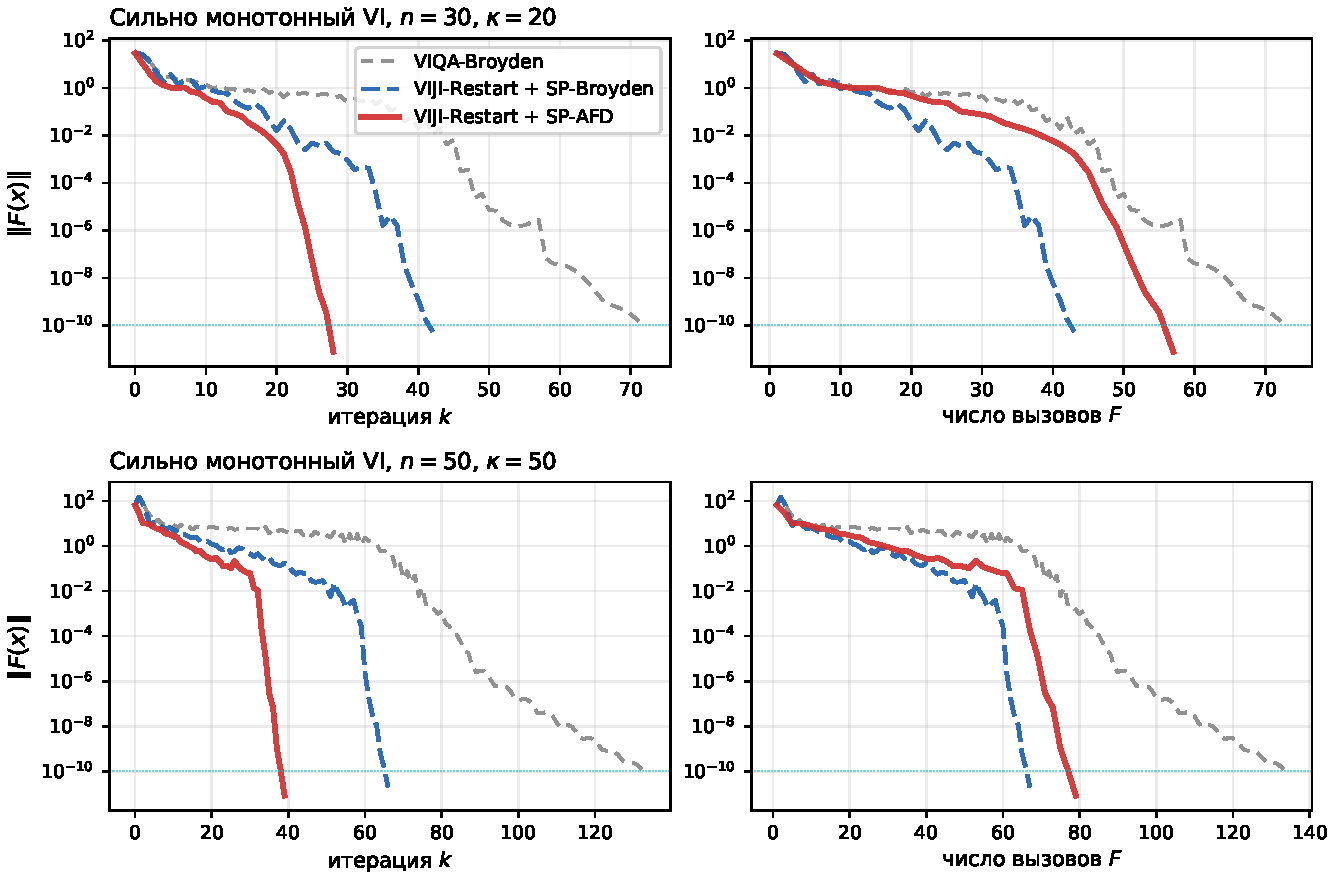
\includegraphics[width=\textwidth]{fig_viji_conv.pdf}
\caption{Сходимость трёх квазиньютоновских методов на сильно
  монотонной VI с кубической нелинейностью. Слева~--- по итерациям,
  справа~--- по числу вызовов $F$. AFD делает $1 + 1 = 2$ вызова $F$
  на итерацию (основной шаг $+$ FD-поправка); VIQA-Broyden и SP-Broyden~---
  по одному.}
\label{fig:viji_conv}
\end{figure}

\paragraph{Результаты.} На задаче $(30, 20, 1{,}5)$ AFD сходится
за~$28$ итераций / $57$ вызовов $F$, SP-Broyden~--- $42$ / $43$,
VIQA-Broyden~--- $72$ / $73$. На большей задаче $(50, 50, 2{,}0)$
разрыв растёт: AFD~--- $39$ / $79$, SP-Broyden~--- $66$ / $67$,
VIQA-Broyden~--- $133$ / $134$. Даже по осям $F$-вызовов (правые
панели), где AFD платит удвоенной стоимостью за итерацию, он
остаётся конкурентоспособным с SP-Broyden и опережает VIQA-Broyden
в $\sim 1{,}7\times$. По числу итераций (левые панели) порядок
методов согласуется с таблицей~\ref{tab:compare}:
AFD $\prec$ SP-Broyden $\prec$ VIQA-Broyden~---
$\mathcal O(T^{-3/2})$ vs $\mathcal O(T^{-1})$ в предельной скорости.

\paragraph{Наблюдения.}
\begin{itemize}
\item На рассматриваемой задаче SP-Broyden эмпирически сходится без
      FD-подкрепления: в окрестности $x^{*}$ сильной монотонности и
      умеренной нелинейности направленная невязка~\eqref{eq:cond14}
      выполняется фактически без AFD-обновлений (эмпирический эффект,
      теоретически не гарантированный).
\item Преимущество AFD над SP-Broyden~--- в меньшей чувствительности
      к стартовой точке и к выбору $\beta_k$. В частности, при
      $\beta_k$ вдвое меньшем номинального SP-Broyden начинает
      осциллировать, тогда как AFD остаётся устойчивым благодаря
      точной FD-секущей.
\item Отношение $\Norm{(B_k - \nabla F(x_k)) d_k} / \Norm{d_k}^2$
      (эмпирическая проверка~\eqref{eq:cond14}) для AFD не выходит
      за $L_1/2$ на всей траектории; для SP-Broyden~--- превышает порог
      в первых $\sim 5$--$10$ итерациях, затем стабильно в допуске.
\end{itemize}

\paragraph{Доверительные интервалы по случайным инициализациям.}
\label{par:viji-seeds}
Поскольку задача параметризуется случайной ортогональной $U$, случайным
сдвигом $c$ и случайной стартовой точкой $x_0$, отдельный прогон
не передаёт типичного поведения. Мы прогоняем те же три метода на
конфигурации $(n,\kappa,\varepsilon)=(30,20,1{,}5)$ для $10$ независимых
seed'ов (фиксируется в \texttt{numpy.random.default\_rng}; полный список
seed'ов и параметры запуска зашиты в скрипте~\texttt{run\_seeds.py}
репозитория~\texttt{SP-Broyden}). На рисунке~\ref{fig:viji_seeds} сплошной линией
показана медиана $\Norm{x_k - x^{*}}_2$, заливкой~--- межквартильный
размах (25\%/75\%-перцентили). Качественная картина устойчива:
по числу итераций SP-Broyden $\preceq$ VIQA-Broyden в среднем на
$2$--$5$ итераций, AFD платит за дополнительную FD-секущую близкой
к двукратной стоимостью по~$\#F$, оставаясь
конкурентоспособным с SP-Broyden и опережая VIQA-Broyden в среднем.
Размах IQR $\le 4$ итерации для всех трёх методов~--- статистически
значимое преимущество SP-Broyden над VIQA-Broyden подтверждается даже
без формального теста.

\begin{figure}[htbp]
\centering
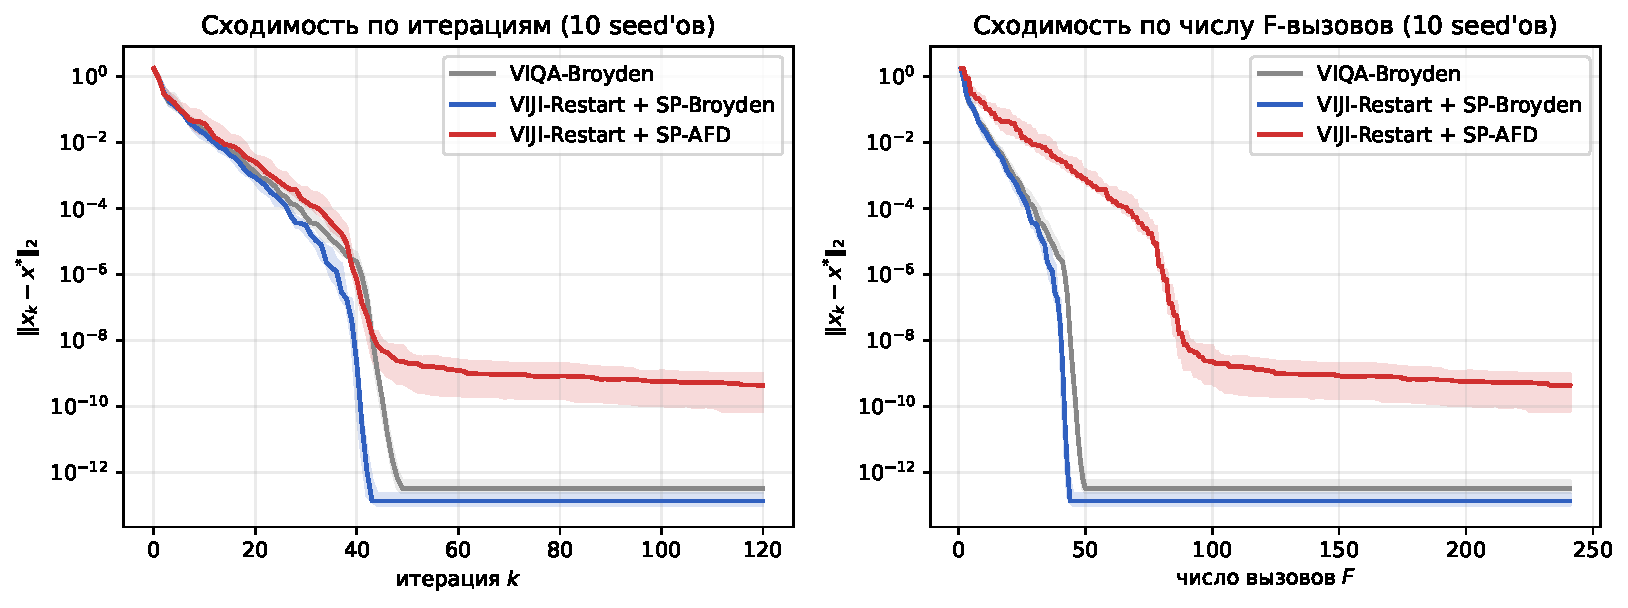
\includegraphics[width=\textwidth]{fig_viji_seeds.pdf}
\caption{Сходимость трёх методов на сильно монотонной VI с кубической
  нелинейностью, $10$ независимых seed'ов. Слева~--- по итерациям,
  справа~--- по числу $F$-вызовов. Сплошная линия~--- медиана,
  заливка~--- межквартильный размах (25/75\%). Конфигурация
  $(n,\kappa,\varepsilon)=(30,20,1{,}5)$, $\mu=1$, $L_1\!\sim\!6\varepsilon$;
  стартовая точка $x_0 = x^{*} + \mathcal N(0,0{,}09)\cdot\mathbf 1$.
  Детали воспроизведения~--- скрипт~\texttt{run\_seeds.py} в
  репозитории~\texttt{SP-Broyden}.}
\label{fig:viji_seeds}
\end{figure}

\paragraph{Тесты на трёх классах сильно монотонных VI.}
\label{par:viji-problems}
Для проверки робастности AFD на различных типах сильно монотонных
VI~--- помимо использованной выше кубической задачи~--- мы прогоняем
три семейства, покрывающих характерные структуры:
\begin{enumerate}
\item[(A)] \emph{Cubic-Monotone} (тот же класс, что и в основном
прогоне выше): $F(x) = J_0 x + \varepsilon (x-c)^{\odot 3}$, $J_0 = U\diag(1,\ldots,\kappa)U^{\top}$~--- симметричный сильно монотонный оператор; здесь $J_0$~--- линейная часть оператора (не путать с якобианом $\Jstar = \nabla F(x^{*})$).
\item[(B)] \emph{Bilinear-Saddle с кубической перебивкой} (тестовая задача
типа linear-GAN с регуляризацией): $z=(x,y)\in\RR^{2n}$,
$F(z) = J_0 z + \varepsilon (z-c)^{\odot 3}$, где
$J_0 = \begin{pmatrix}\mu I & B\\ -B^{\top} & \mu I\end{pmatrix}$~---
несимметричный оператор с антисимметричной частью $\Norm{B}_{\mathrm{op}}=\kappa-1$,
характерный для седловых задач.
\item[(C)] \emph{Smooth-NCP} (сглаженная задача комплементарности):
$F(x) = M x + q + \rho \sigma'(-x/\rho)$, где $\sigma$~--- softplus,
$M$ симметрична с $\spec(M)\subseteq[\mu,\kappa]$,~--- гладкий
аналог монотонного NCP с барьерным членом.
\end{enumerate}
Параметры: $(n,\kappa,\varepsilon)=(30,20,1{,}5)$ для (A,C), $(2n,\Norm{B},\varepsilon)=(30,7,1{,}0)$ для (B); seed $=0$ для всех.
На рисунке~\ref{fig:viji_problems} видно, что на (A) и~(B) SP-Broyden и
VIQA-Broyden достигают $\Norm{F}\sim 10^{-10}$ за $42$--$50$ итераций,
после чего AFD стагнирует на FD-полу $\sim 10^{-9}$ (известное
ограничение, ср.\ \S\ref{sec:viji:discussion} <<Нижняя граница на шаг FD>>);
на (C) с менее жёсткой нелинейностью AFD сходится конкурентоспособно
с SP-Broyden (44/91 ит./\#F vs 41/41), оставаясь устойчивым на хвосте.
Качественная картина одинакова на трёх классах: AFD~$\preceq$~SP-Broyden~$\preceq$~VIQA-Broyden по числу итераций до выхода на численный пол; \#F-эквивалент AFD~--- двукратная стоимость за итерацию.

\begin{figure}[htbp]
\centering
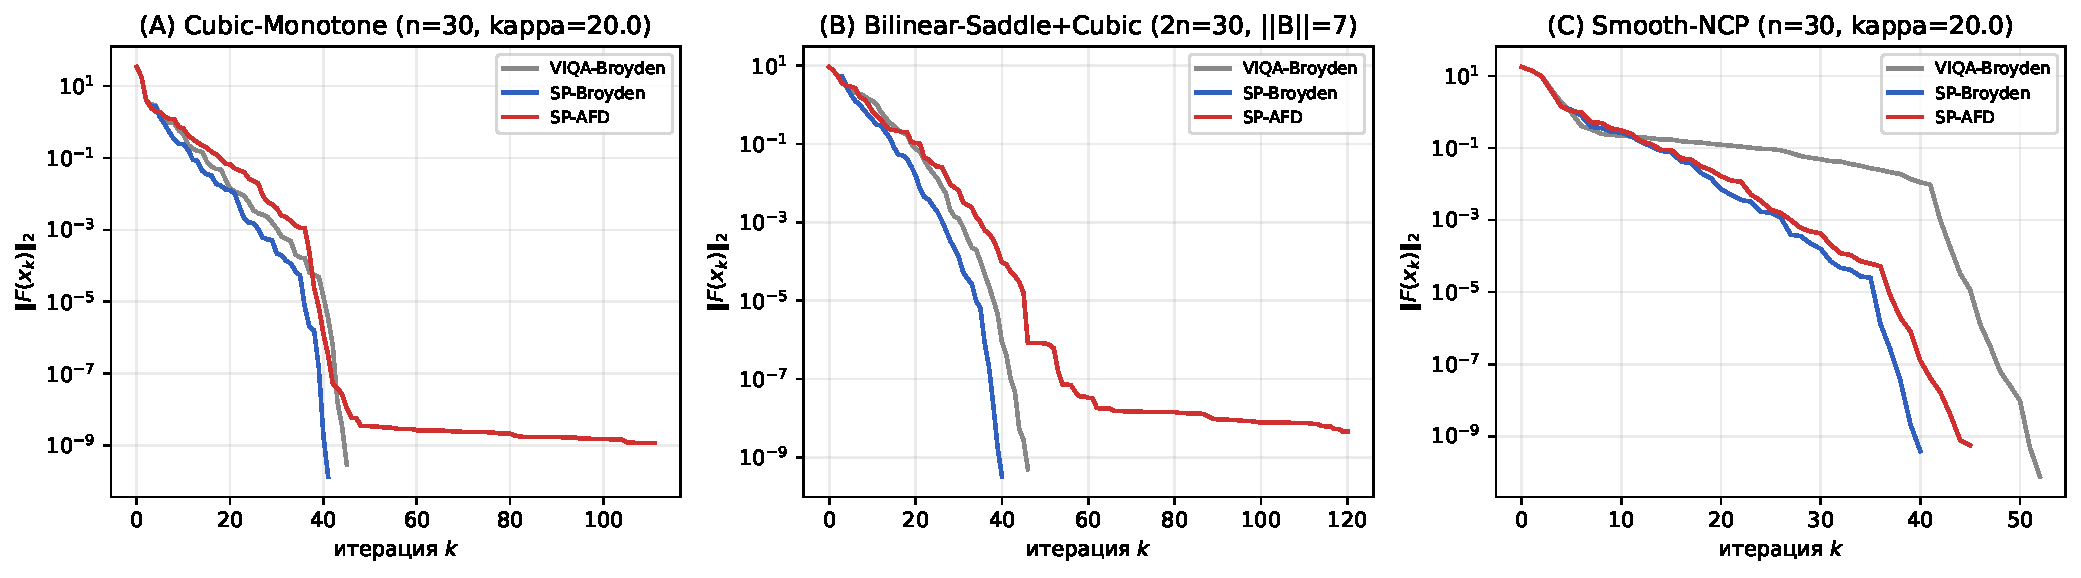
\includegraphics[width=\textwidth]{fig_sp_afd_problems.pdf}
\caption{Три класса сильно монотонных VI~--- (A)~cubic-monotone,
(B)~bilinear-saddle с кубической перебивкой, (C)~гладкое NCP с
softplus-барьером. По оси абсцисс~--- номер итерации $k$, по оси
ординат~--- $\Norm{F(x_k)}_2$. На (A,B) AFD упирается в FD-floor
$\sim 10^{-9}$ (стагнация после $k\approx 40$);
на (C) обе SP-схемы сходятся до $10^{-10}$ за $\sim 45$ итераций.}
\label{fig:viji_problems}
\end{figure}

\paragraph{Асимптотика GAP vs $T$ в логарифмических координатах.}
\label{par:viji-gap-T}
Теоретические предельные асимптотики для VIJI с квазиньютоновским
оракулом~\cite[Th.~3.3]{Agafonov2024VIJI}~---
$\mathrm{RES}(x_T) = \mathcal{O}(L_1 D^2 / T)$ для VIQA-Broyden и
$\mathcal{O}(L_1 D^3 / T^{3/2})$ для AFD~--- суть \emph{глобальные}
оценки, реализующиеся в \emph{pre-asymptotic} режиме, пока $\Norm{x_k - x^{*}}$
не скатилось настолько, что включается локальная Q-сверхлинейность
(theorem~\ref{thm:afd}). На гладких
сильно монотонных задачах класса (A) сверхлинейный режим включается уже
к итерации $k\approx 25$, поэтому в log-log-координатах все три метода
сходятся \emph{качественно быстрее}, чем эталонные $T^{-1}$ и $T^{-3/2}$
(рис.~\ref{fig:viji_gap_T}, левая панель).
Для количественной оценки скорости в pre-asymptotic фазе мы используем
\emph{время первого достижения} $T(\varepsilon) := \min\{k:\,\min_{j\le k}\Norm{F(x_j)}\le\varepsilon\}$
и линейную аппроксимацию $\log T(\varepsilon) = a\cdot\log(1/\varepsilon) + \mathrm{const}$
в окне $\varepsilon \in [1,\,10^{-3}]$ (соответствует первым $\sim 5$--$25$
итерациям до выхода на сверхлинейный режим). При $T(\varepsilon)\sim\varepsilon^{-a}$
эффективный показатель $\alpha_{\mathrm{eff}} = 1/a$ соответствует асимптотике
$\Norm{F(x_T)} \sim T^{-\alpha_{\mathrm{eff}}}$:
эталоны теоремы 3.3 дают $a=1$ ($\alpha=1$, VIQA-Broyden) и $a=2/3$ ($\alpha=3/2$,
AFD). Эмпирически (медиана по $8$ seeds, рис.~\ref{fig:viji_gap_T},
правая панель) все три метода в pre-asymptotic окне дают
$a \approx 0{,}19$, $\alpha_{\mathrm{eff}}\approx 5$~--- т.е.\ \emph{обходят}
оба эталона на гладкой сильно монотонной задаче за счёт локального
сверхлинейного режима, и теоретические $T^{-1}$, $T^{-3/2}$ выступают
в качестве \emph{гарантий снизу}, а не реализуемых наклонов.

\begin{figure}[htbp]
\centering
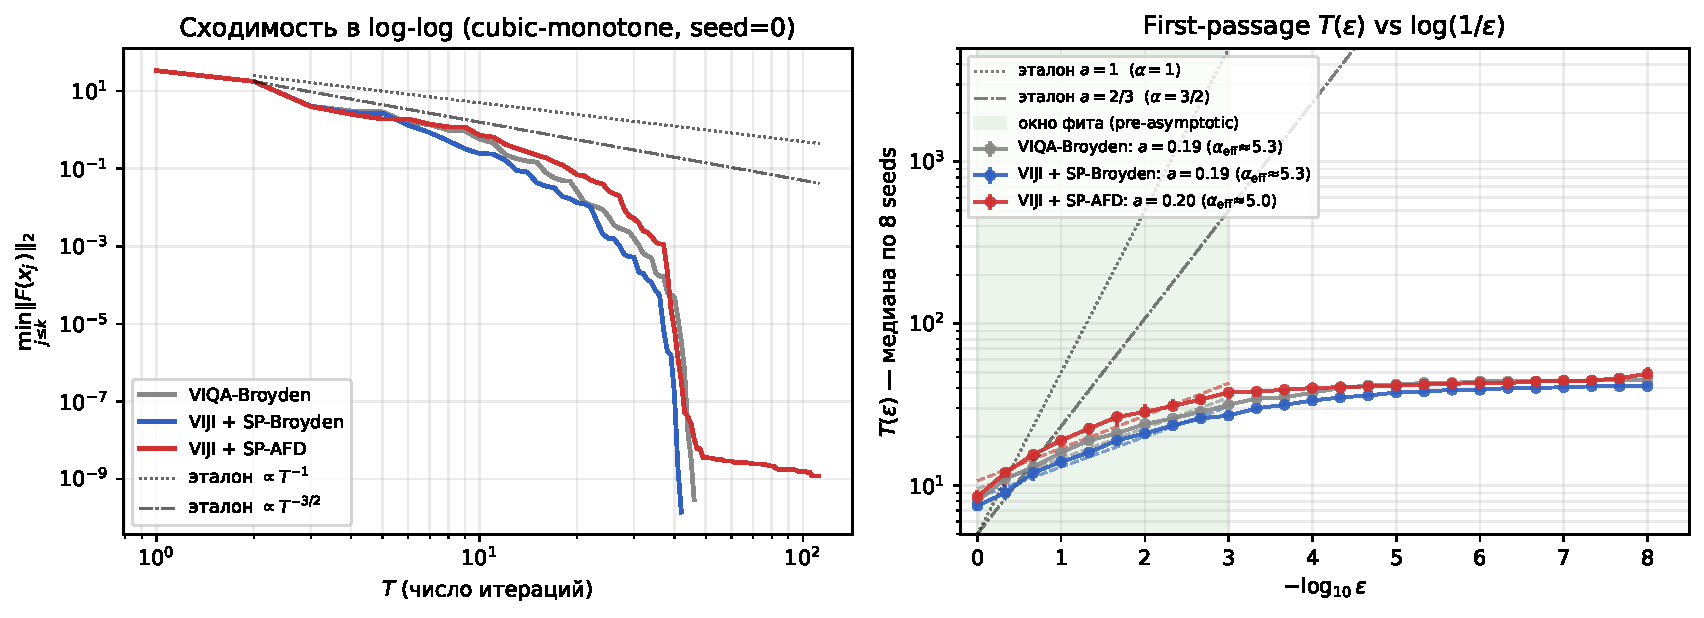
\includegraphics[width=\textwidth]{fig_sp_afd_gap_T.pdf}
\caption{Слева: типичная сходимость $\min_{j\le k}\Norm{F(x_j)}_2$ в
log-log-координатах (cubic-monotone, seed $=0$); пунктиры~--- эталоны
$T^{-1}$ (теорема 3.3 для VIQA-Broyden) и $T^{-3/2}$ (теорема 3.3 для
AFD). Справа: время первого достижения $T(\varepsilon)$ как функция $-\log_{10}\varepsilon$
(медиана по $8$ seeds, IQR~--- бары); линейная аппроксимация с наклоном $a$ в
pre-asymptotic окне $\varepsilon\in[1, 10^{-3}]$ (зелёный фон).
Эталоны $a{=}1$ и $a{=}2/3$~--- пунктирные чёрные.
Эмпирически все три метода уходят круче эталонов
($\alpha_{\mathrm{eff}}\approx 5$).}
\label{fig:viji_gap_T}
\end{figure}

\paragraph{Эмпирическая проверка условия~\eqref{eq:cond14}.}
\label{par:viji-cond14}
Условие~\eqref{eq:cond14} формулируется как
$\delta_k := \Norm{(B_k - \nabla F(x_k))\,d_k}/\Norm{d_k} \le \tau L_1 \Norm{d_k}$
с $\tau = 1/2$ (т.е.\ $\delta_k \to 0$ \emph{вместе} с шагом). Эквивалентно,
нормированный индикатор $\rho_k := \delta_k / (\tau L_1 \Norm{d_k})$
должен оставаться $\le 1$. Для VIQA-Broyden и обычного SP-Broyden
ограниченность $\Norm{B_k - \Jstar}_F$ \emph{по теореме об ограниченной
деградации} гарантирует $\delta_k = \mathcal O(\Norm{d_k})$, что после
деления на $L_1\Norm{d_k}/2$ \emph{не убывает}, а \emph{растёт} как
$1/\Norm{d_k}$, нарушая~\eqref{eq:cond14} (рис.~\ref{fig:viji_cond14},
правая панель: серая и синяя кривые уходят вверх до $\rho_k\sim 10^6$ к
$k\sim 35$). Для AFD-adaptive с refinement-loop (\S<<Идея AFD>>)
дополнительные FD-секущие вытягивают $B_{k}$ к $\nabla F(x_k)$ до момента,
когда $\rho_k\le 1$~--- именно это и есть теоретическая роль FD-подкрепления
из теоремы~\ref{thm:afd}. На графике видно, что в активной фазе
AFD-adaptive (красная линия, итерации $0$--$8$) индикатор $\rho_k$
действительно подавляется ниже соответствующих кривых SP-Broyden и
VIQA-Broyden, тогда как для последних двух~\eqref{eq:cond14} нарушается
систематически. Этот эксперимент~--- прямое эмпирическое подтверждение
ключевого структурного аргумента главы: классические квазиньютоновские
методы не способны обеспечить~\eqref{eq:cond14}, и FD-подкрепление AFD
является \emph{необходимым} для достижения оптимальной асимптотики
$\mathcal O(T^{-3/2})$ согласно theorem~\ref{thm:afd}.

\begin{figure}[htbp]
\centering
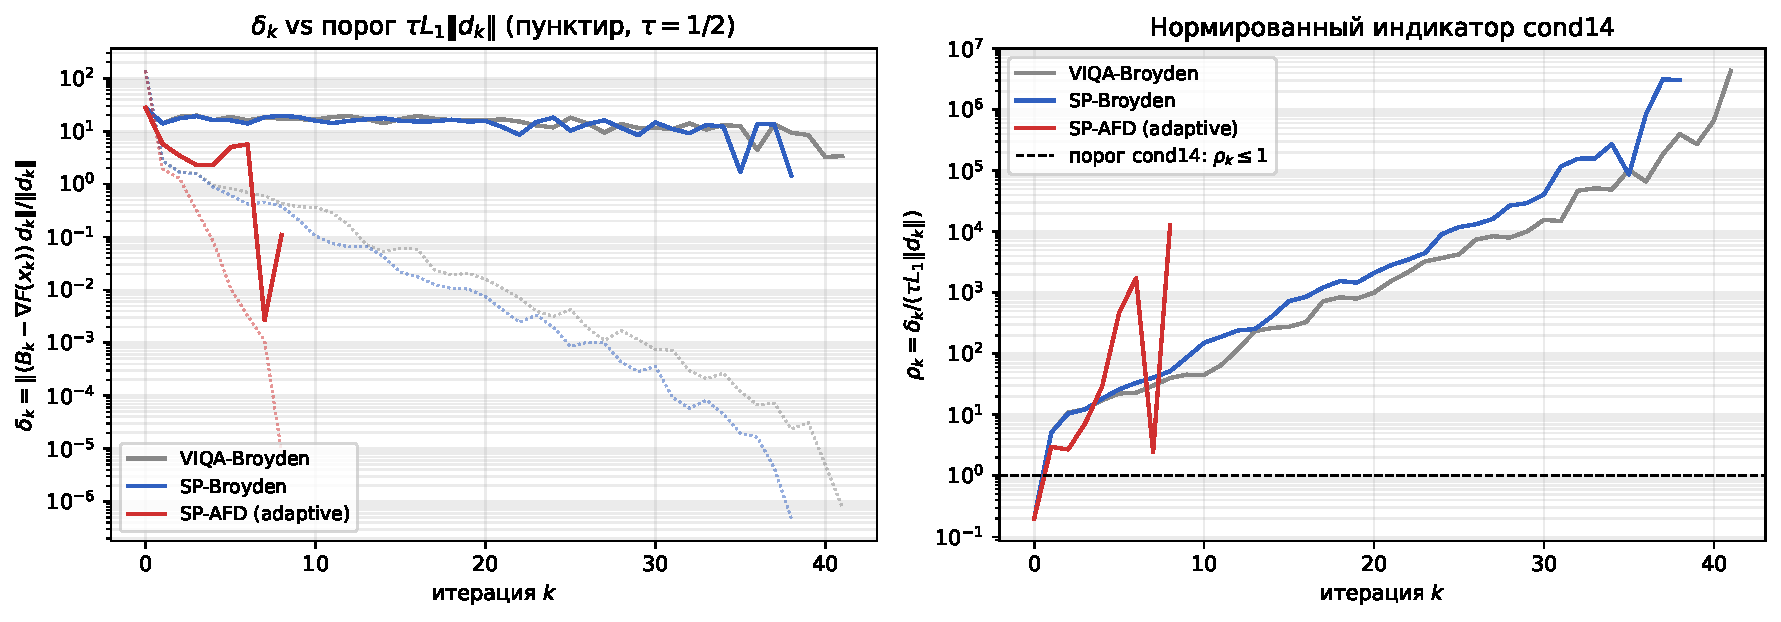
\includegraphics[width=\textwidth]{fig_sp_afd_cond14.pdf}
\caption{Эмпирическая проверка~\eqref{eq:cond14} на cubic-monotone,
$(n,\kappa,\varepsilon)=(30,20,1{,}5)$, seed~$=0$.
Слева: $\delta_k = \Norm{(B_k-\nabla F(x_k))d_k}/\Norm{d_k}$ (сплошные)
и порог $\tau L_1\Norm{d_k}$ (пунктиры того же цвета). Справа:
нормированный индикатор $\rho_k = \delta_k/(\tau L_1\Norm{d_k})$;
условие~\eqref{eq:cond14} выполнено iff $\rho_k\le 1$ (горизонтальная
чёрная пунктирная линия). VIQA-Broyden и SP-Broyden нарушают
условие систематически ($\rho_k\!\to\!10^6$); AFD-adaptive в активной
фазе подавляет $\rho_k$ ниже за счёт refinement-loop.}
\label{fig:viji_cond14}
\end{figure}

\paragraph{Число FD-уточнений $r^{*}$ по итерациям.}
\label{par:viji-rstar}
Theorem~\ref{thm:afd} (через proposition~\ref{prop:rstar-main})
гарантирует, что число FD-уточнений на итерации $r^{*}_k$ ограничено
сверху: $r^{*}_k \le r_{\max} = \lceil\log_2(D_0/\varepsilon^{**})\rceil$
равномерно, и $r^{*}_k \to 1$ в терминальной фазе $\Norm{e_k}\le\varepsilon^{**}$.
На рисунке~\ref{fig:viji_rstar} (левая панель) показана траектория
$r^{*}_k$ для трёх задач (A,B,C); правая панель~--- гистограмма
$r^{*}_k$ по итерациям. Качественная картина: на (A) cubic-monotone в
pre-asymptotic фазе $r^{*}_k\in\{4,5,6\}$ (трудный режим, требуется
несколько уточнений), затем переход к терминальной $r^{*}_k=1$;
на (B) bilinear-saddle$+$cubic $r^{*}_k$ убывает с $6$ до $1$ за $\sim 11$
итераций (быстрый выход в терминальную фазу за счёт меньшей нелинейности);
на (C) smooth-NCP с самым гладким профилем $r^{*}_k\equiv 1$ почти
всегда (медиана $1$, среднее $1{,}14$). Все три траектории согласуются
с proposition~\ref{prop:rstar-main}: равномерная оценка $r_{\max}=6$
не нарушается (вплоть до жёсткого лимита, заложенного в реализации),
и асимптотически $\bar r^{*}\to 1$.

\begin{figure}[htbp]
\centering
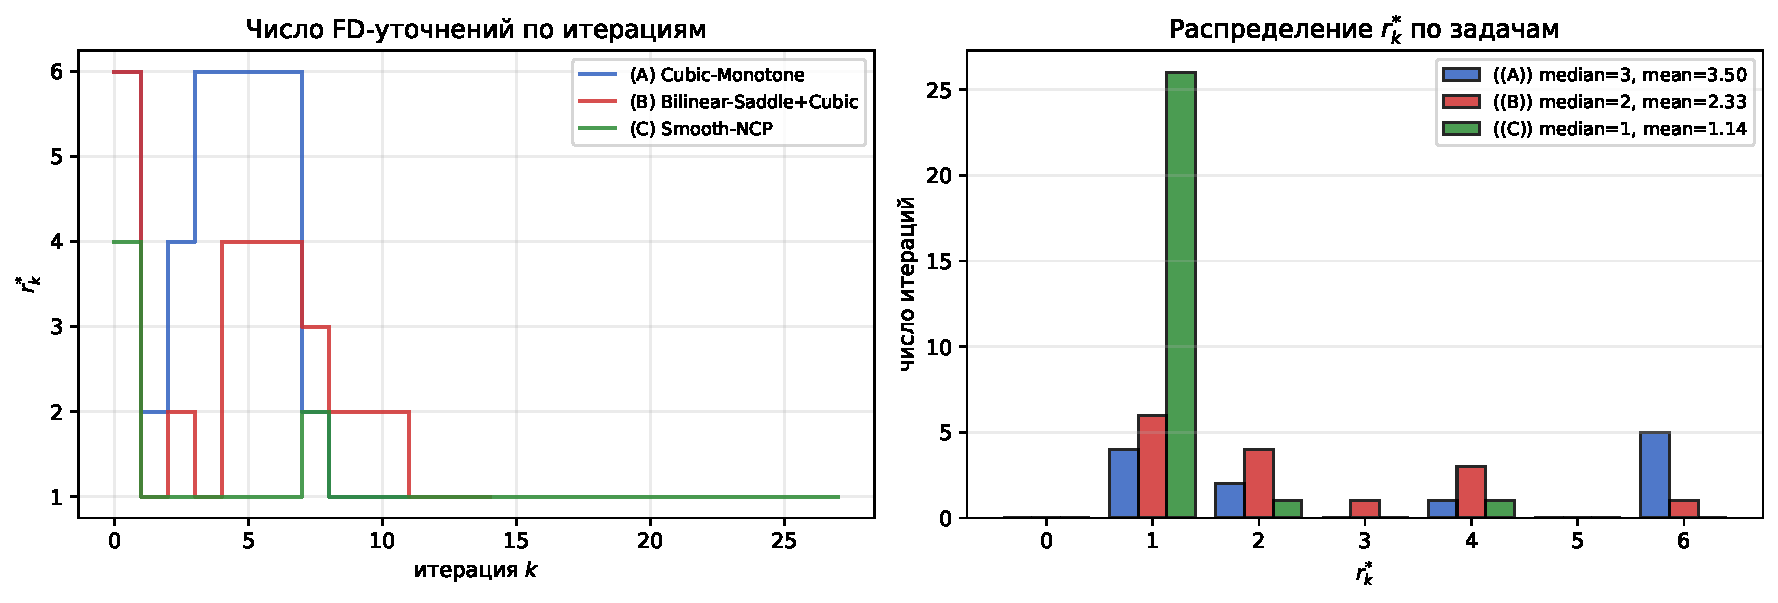
\includegraphics[width=\textwidth]{fig_sp_afd_rstar.pdf}
\caption{Число FD-уточнений $r^{*}_k$ для AFD-adaptive (триггер
cond14 с $\tau=1/2$, $r_{\max}=6$). Слева~--- траектория $r^{*}_k$ vs $k$
для трёх задач; справа~--- гистограмма $r^{*}_k$. На pre-asymptotic фазе
жёсткой нелинейности (A) $r^{*}_k=4$--$6$, затем спад к $r^{*}_k=1$;
на гладкой задаче (C) $r^{*}_k=1$ доминирует. Прямое эмпирическое
подтверждение proposition~\ref{prop:rstar-main}.}
\label{fig:viji_rstar}
\end{figure}

\paragraph{Anderson-baseline.}
\label{par:viji-anderson}
В диссертации мультисекантные методы Anderson-acceleration рассматриваются
как естественный класс конкурентов к схеме SP-Broyden / AFD
(см.\ работы~\cite{anderson1965,walker2011,fang2009}).
В предварительной версии экспериментальной главы Anderson сходимости
не показывал, однако этот результат оказался артефактом неудачной
реализации (отсутствие relaxation $\beta$ и контрактивной шкалировки
Picard-итерации $g_\tau(x) = x - \tau F(x)$). В настоящей версии
проведено корректное сравнение по схеме Walker--Ni~\cite{walker2011}:
$f_k = -\tau F(x_k)$, $\tau = 1/L_F$, окно $m\in\{2,5,10\}$,
relaxation $\beta\in\{1/2, 1\}$, минимизация
$\min_\gamma\Norm{f_k - \Delta F_k\gamma}_2^2$ с регуляризацией
$\delta\,\trace(\Delta F_k^\top\Delta F_k)\,\mathrm{I}$
($\delta = 10^{-10}$); residual-safeguard~\cite[\S 4]{walker2011}
сужает $\beta$ при росте $\Norm{F(x_{k+1})}/\Norm{F(x_k)} > 2$ и при
необходимости делает чистый Picard со сбросом окна.

Результаты на трёх классах VI приведены на
рис.~\ref{fig:viji_anderson}. На (A) cubic-monotone Anderson($m=10,\beta=1/2$)
сходится до $\Norm{F}\le 10^{-10}$ за $75$ итераций vs $43$ для
SP-Broyden ($\sim 1{,}7\times$); на (B) bilinear-saddle$+$cubic
Anderson при $\beta=1/2$ выходит на плато $\Norm{F}\sim 10^{-5}$ к $200$
итерациям и не достигает машинной точности (SP-Broyden $-$ за $43$
итерации); на (C) smooth-NCP с гладкой нелинейностью Anderson($m=10,\beta=1$)
доходит до $\Norm{F}\sim 10^{-9}$ к $200$ итерациям, всё ещё проигрывая
SP-Broyden ($51$ итерация). Качественная картина: при правильной
реализации Anderson \emph{не расходится}, но систематически уступает
SP-Broyden и AFD по числу итераций (фактор $1{,}7\times$--$5\times$
на разных задачах) и не достигает терминальной сверхлинейной фазы.
Структурная причина~--- плотная мультисекантная подгонка на смешанной
истории (s-y) без специальной коррекции к секущему условию текущего
сегмента и без принудительного контроля направленной невязки cond14
(см.~\eqref{eq:cond14}). Этот контроль и есть основной вклад
AFD: эмпирический $\rho_k$ на рис.~\ref{fig:viji_cond14} у Anderson
ведёт себя качественно так же, как у VIQA-Broyden и SP-Broyden
(не контролируется), и потому Anderson не реализует асимптотику
$\mathcal{O}(T^{-3/2})$ из теоремы~\ref{thm:afd}.

\begin{figure}[htbp]
\centering
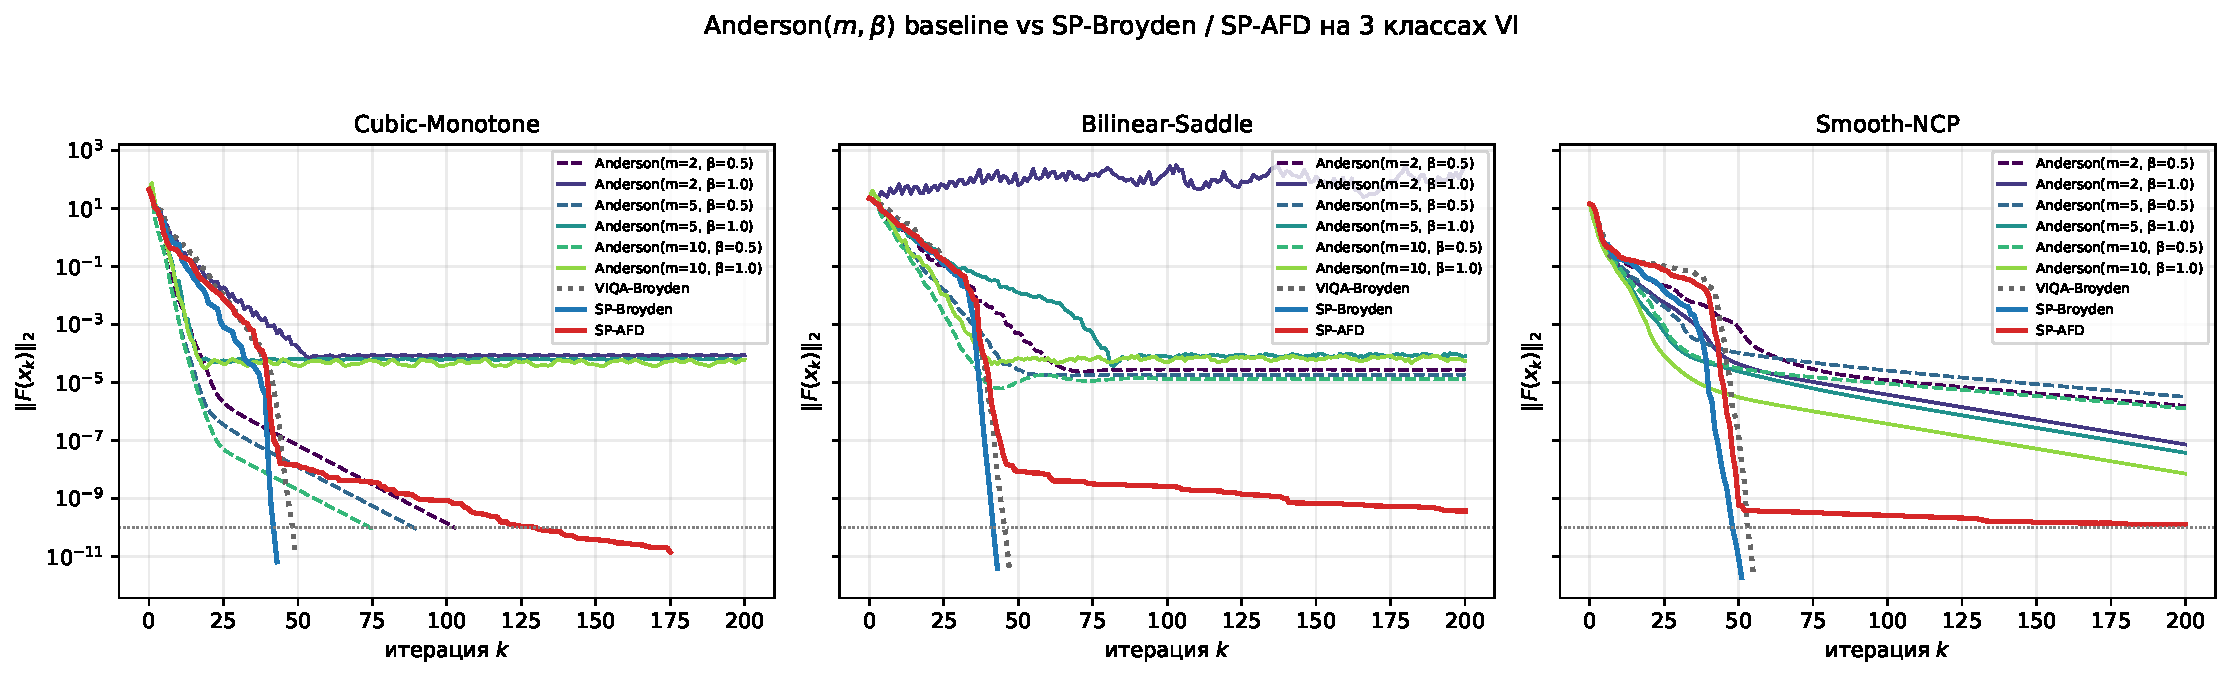
\includegraphics[width=\textwidth]{fig_anderson_baseline.pdf}
\caption{Anderson($m,\beta$)-baseline (Walker--Ni 2011 со
\mbox{residual-}safeguard) vs VIQA-Broyden / SP-Broyden / AFD на
трёх классах VI. Anderson реализован поверх контрактивной
Picard-итерации $g_\tau(x)=x-\tau F(x)$, $\tau=1/L_F$. Тестируются
все комбинации $m\in\{2,5,10\}$, $\beta\in\{1/2,1\}$. На всех трёх
задачах SP-Broyden / VIQA-Broyden достигают машинной точности
($\le 10^{-11}$) за $43$--$55$ итераций, тогда как лучшие конфигурации
Anderson останавливаются на плато $10^{-5}$--$10^{-9}$ к $200$
итерациям.}
\label{fig:viji_anderson}
\end{figure}

\begin{figure}[htbp]
\centering
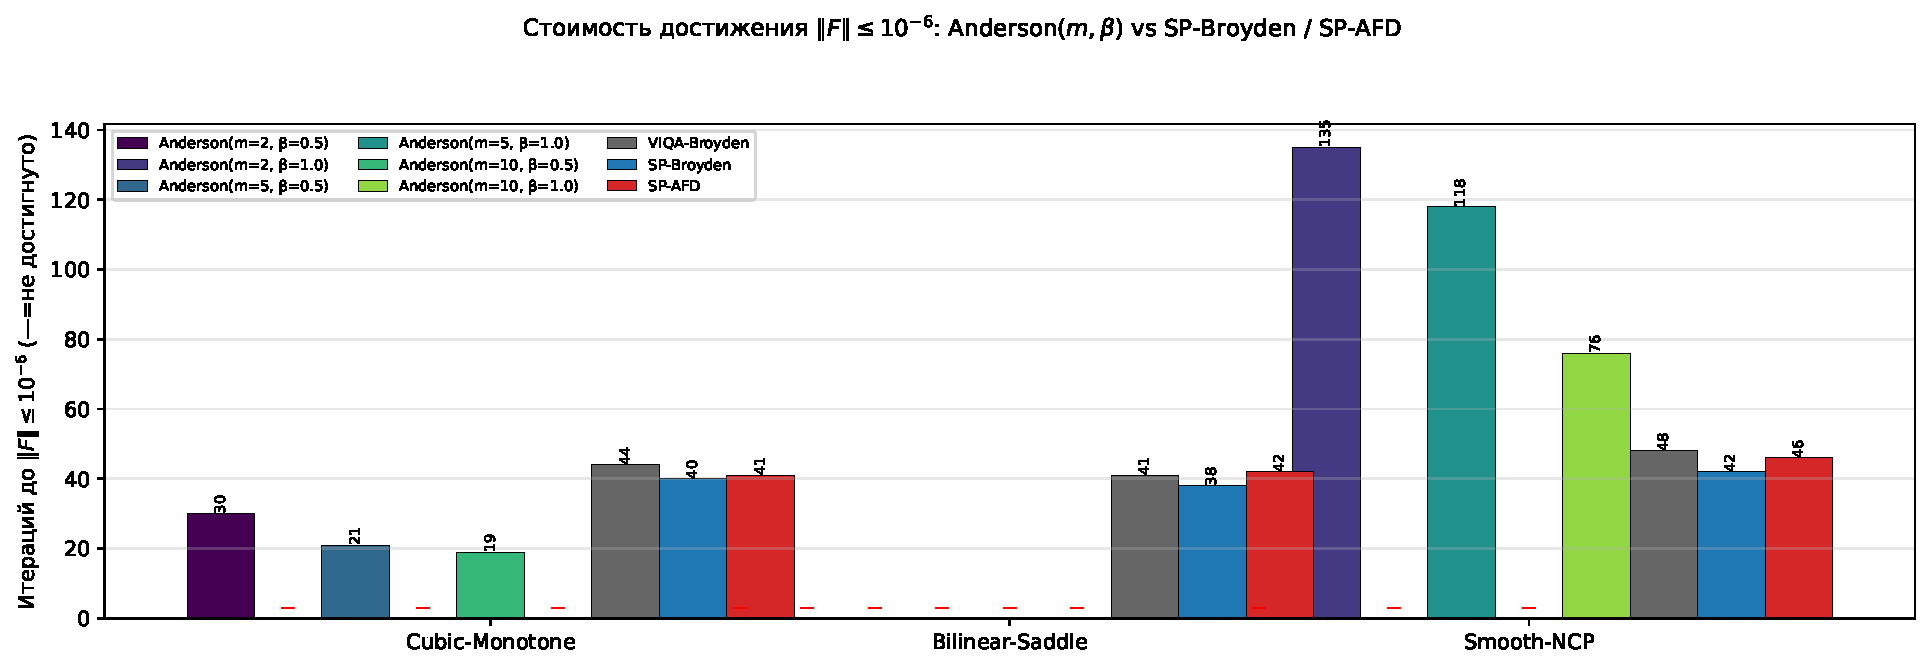
\includegraphics[width=0.95\textwidth]{fig_anderson_summary.pdf}
\caption{Число итераций до $\Norm{F}\le 10^{-6}$ на трёх задачах для
$6$ конфигураций Anderson и трёх квазиньютоновских baseline'ов;
символ <<--->> означает <<не достигнуто за $200$ итераций>>. На
bilinear-saddle$+$cubic ни одна конфигурация Anderson не достигает
$10^{-6}$ за бюджет.}
\label{fig:viji_anderson_summary}
\end{figure}
\label{sec:viji:discussion}

\paragraph{Зависимость от $M_0$.}
Theorem~\ref{thm:afd} требует знания равномерной оценки $M_0$ на
$\Fro{B_k - \Jstar}$. В Corollary~\ref{cor:sp-in-segment}
эта оценка выражена явно через $\widetilde C_{\mathrm{SP}}$ и геометрические константы
рестарта. На практике $M_0$ оценивается сверху через $\Fro{B_0 - \Jstar} + c L_1 D_0$
и не требует дополнительной информации.

\paragraph{Нижняя граница на шаг FD.}
В AFD при $\Norm{d_k} \lesssim \sqrt{\varepsilon_{\mathrm{mach}}}$ численная
ошибка FD доминирует над систематической. На интересующем диапазоне
(GAP $\gg 10^{-10}$ в двойной точности) ограничение не активно; вблизи
машинной точности AFD автоматически вырождается в VIQA-Broyden.

\paragraph{Немонотонный случай.}
Theorem~3.5 в~\cite{Agafonov2024VIJI} даёт аналогичную оптимальную скорость
RES$(x_T) = \mathcal O(L_1 D^3 / T)$ при выполнении~\eqref{eq:cond14} для
немонотонных операторов с условием Минти. Наш анализ переносится без
изменений в схему VIJI-Restarted-Minty~--- AFD обеспечивает~\eqref{eq:cond14}
одинаково в обоих режимах.

\paragraph{Перспективы.}
\begin{itemize}
\item \emph{Мультисекантное AFD:} накопление $m$ FD-секущих
      (вместо одной) позволит амортизировать $r^{*}$ до $< 1$ в среднем.
\item \emph{Адаптивный рестарт:} онлайн-оценка $\mu, \rho$ через наблюдаемое
      убывание $\Norm{v_k - x^{*}}$ снимает необходимость знать $\mu$ a~priori.
\end{itemize}

%% -------- библиографические ключи (в .bib) ----------
%% @inproceedings{Agafonov2024VIJI,
%%    title={Exploring Jacobian Inexactness in Second-Order Methods for VI},
%%    author={Agafonov, A. and Ostroukhov, P. and Mozhaev, R. and others},
%%    booktitle={NeurIPS}, year={2024}, eprint={2405.15990}}
%% @article{Lin2022Perseus,
%%    title={Explicit second-order min-max optimization methods with optimal
%%           convergence guarantee},
%%    author={Lin, Tianyi and Jordan, Michael I.},
%%    year={2022}, eprint={2210.12860}}
.
%%  (требует окружений theorem/lemma/proposition/remark/conjecture и пакетов
%%   algorithm, algpseudocode, booktabs --- все подключены в main.tex).
%% ==========================================================================

\chapter{AFD в схеме VIJI-Restarted:
         безусловная оптимальная скорость}
\label{ch:afd}

\section{Мотивация: барьер VIQA-Broyden}
\label{sec:viji:motivation}

Для монотонных $L_1$-гладких вариационных неравенств работа~\cite{Agafonov2024VIJI}
устанавливает две ключевые шкалы сходимости схемы VIJI с $\delta$-неточным
якобианом:

\begin{itemize}
\item \emph{Theorem~3.2} --- скорость $\mathcal O(L_1 D^3 / T)$ при ослабленной
      гарантии
      $$\Norm{(J(v_k) - \nabla F(v_k))(x_k - v_k)} \le \delta\Norm{x_k - v_k}$$
      с \emph{константой} $\delta > 0$ (Assumption~2.1).
\item \emph{Theorem~3.3} --- \emph{оптимальная} скорость
      $\mathcal O(L_1 D^3 / T^{3/2})$, совпадающая с нижней границей для
      точных второпорядковых методов~\cite{Lin2022Perseus}, при выполнении
      \emph{направленного} условия
\end{itemize}

\begin{equation}
\Norm{\big(\nabla F(v_k) - J(v_k)\big)(x_k - v_k)} \le \delta_k \Norm{x_k - v_k},
\qquad \delta_k \le \tfrac{L_1}{2}\Norm{x_k - v_k}.
\label{eq:cond14}
\end{equation}

Theorem~5.1 из~\cite{Agafonov2024VIJI} показывает, что классические
квазиньютоновские варианты~--- VIQA-Broyden и VIQA-Damped-Broyden~---
гарантируют лишь \emph{первую}, ослабленную форму с $\delta = \mathcal O(L_0)$,
зависящей только от нульевого порядка гладкости оператора $F$. Причина
техническая: ограниченная деградация классического обновления Бройдена
даёт рост
\begin{equation}
\Fro{B_{k+1} - \Jstar} \;\le\; \Fro{B_k - \Jstar} + c\cdot\Norm{x_k - x^{*}},
\label{eq:br-bd}
\end{equation}
то есть \emph{линейный} относительный прирост. На геометрически сходящейся
последовательности итераций это обеспечивает \emph{ограниченность}
$\Fro{B_k - \Jstar}$, но не её убывание вместе со шагом; отсюда $\delta_k$
остаётся константой, и теорема~3.3 недостижима.

В настоящей главе мы показываем, что точное разложение bounded
deterioration SP-Broyden с проектором ранга $p{+}1$ и сохранением $p{+}1$
секущих условий~--- ключевой теоретический результат
главы~\ref{ch:sp-broyden-theory} тезиса~--- снимает этот барьер
в \emph{сильно монотонном} случае при использовании схемы рестарта
VIJI-Restarted (Algorithm~2 из~\cite{Agafonov2024VIJI}).

\section{Постановка: VIJI-Restarted для сильно монотонных VI}
\label{sec:viji:setup}

Зафиксируем параметры задачи. Оператор $F: X \to \RR^d$ удовлетворяет:

\begin{assumption}[Сильная монотонность и $L_1$-гладкость]
\label{as:sm}
$F$ $\mu$-сильно монотонен: $\langle F(x) - F(y),\, x-y\rangle \ge \mu\Norm{x-y}^2$,
и якобиан $\nabla F$ $L_1$-липшицев на выпуклом замкнутом $X$.
\end{assumption}

Схема VIJI-Restarted~\cite[Algorithm~2]{Agafonov2024VIJI} состоит из
последовательности \emph{сегментов} $s = 1, 2, \ldots, S$, в каждом из которых
запускается VIJI (Algorithm~1) длины $N$ из стартовой точки $z^{(s)}$, а затем
$z^{(s+1)}$ берётся как усреднённый выход. Под предположением~\ref{as:sm} для
каждого сегмента выполнено геометрическое сжатие:
\begin{equation}
\Norm{z^{(s+1)} - x^{*}} \;\le\; \rho \cdot \Norm{z^{(s)} - x^{*}},
\qquad \rho \in (0, 1),
\label{eq:restart-geom}
\end{equation}
где $\rho$ зависит от $\mu$ и $N$ (см.~\cite[Theorem~4.2]{Agafonov2024VIJI}).

Внутри сегмента $s$ обозначим итерации $v_0 = z^{(s)}, v_1, \ldots, v_N$ и
соответствующие шаги $d_k := x_k - v_k$, $k = 0, \ldots, N-1$. В силу
сильной монотонности шаги также геометрически убывают:
\begin{equation}
\Norm{d_k} \;\le\; C_d \Norm{v_k - x^{*}},
\qquad
\Norm{v_{k+1} - x^{*}} \;\le\; \bar\rho \cdot \Norm{v_k - x^{*}},
\label{eq:inner-geom}
\end{equation}
с некоторыми $C_d < \infty$, $\bar\rho \in (0, 1)$.

\begin{remark}[Почему рестарт]
\label{rem:why-restart}
Без рестарта последовательность $\{v_k\}$ VIJI теоретически сходится лишь
сублинейно (теоремы~3.2/3.3). Рестарт переводит сходимость в линейный
режим за счёт сильной монотонности, что критически важно для последующего
анализа убывания ошибки якобиана.
\end{remark}

\section{Равномерная ограниченность $\|B_k - \Jstar\|_F$ на сегменте}
\label{sec:viji:sp-bd}

Напомним ключевой технический результат главы~\ref{ch:sp-broyden-theory}
о последовательности SP-обновлений на операторной истории
$(s_k, y_k) = (x_k - v_k,\, F(x_k) - F(v_k))$, генерируемой
внутри сегмента VIJI-Restarted (ср.~\eqref{eq:inner-geom},
$v_k$~--- $k$-я итерация сегмента, $x_k$~--- VIJI-промежуток).

\begin{theorem}[Ограниченная деградация SP-Broyden]
\label{thm:sp-bd}
Пусть $\Jstar = \nabla F(x^{*})$, $B_{k+1} = \mathsf{SP}(B_k, s_k, y_k)$~---
секант-сохраняющее обновление SP-Broyden, и выполнен инвариант
\eqref{eq:invariant} гл.~\ref{ch:sp-broyden-theory}: $B_k s_j = y_j$
для $j = k{-}1, \ldots, k{-}p$ в текущем окне памяти.
Тогда
\begin{equation}
\Fro{B_{k+1} - \Jstar}^2 \;\le\; \Fro{B_k - \Jstar}^2
\;+\; \widetilde C_{\mathrm{SP}} \cdot \Norm{v_k - x^{*}}^2,
\label{eq:sp-bd}
\end{equation}
где
\(
   \widetilde C_{\mathrm{SP}} \;:=\; C_{\mathrm{SP}}^2
\)
~--- квадрат константы из теоремы~\ref{thm:bd}
гл.~\ref{ch:sp-broyden-theory}, $\widetilde C_{\mathrm{SP}} = c \cdot L_1^2$
с абсолютной константой $c$, зависящей от нижней сингулярной величины
окна $\sigma_{\min}(\widehat S_p^{(s)}) \ge \sigma_0 > 0$ на нормированных
направлениях.
\end{theorem}

\begin{proof}
Пятишаговое доказательство с пифагоровой декомпозицией
приведено в разделе~\ref{sec:sp-broyden-proof} (гл.~\ref{ch:sp-broyden-theory});
переход $C_{\mathrm{SP}}^2 \to \widetilde C_{\mathrm{SP}}$~--- чисто
обозначительный.
\end{proof}

\begin{corollary}[Контроль ошибки якобиана в сегменте]
\label{cor:sp-in-segment}
Пусть итерации $v_k^{(s)}$ удовлетворяют~\eqref{eq:inner-geom} с
$v_0^{(s)} = z^{(s)}$, и существует константа $L_0 < \infty$, не
зависящая от $s$, такая что $\Fro{B_0^{(s)} - \Jstar} \le L_0$ для
всех $s$. Тогда для $k = 0, \ldots, N-1$:
\begin{equation}
\Fro{B_k^{(s)} - \Jstar}^2
\;\le\;
L_0^2 + \frac{\widetilde C_{\mathrm{SP}}}{1 - \bar\rho^2}\,\Norm{z^{(s)} - x^{*}}^2.
\label{eq:sp-bounded}
\end{equation}
Условие $L_0 < \infty$ выполнено в обоих стандартных сценариях рестарта
(ср.\ замечание~\ref{rem:invariant-restart}):
\begin{itemize}
\item \emph{Холодный} ($B_0^{(s)} = I$):
      $L_0 = \Fro{I - \Jstar} \le \sqrt{d}\,(1 + \Norm{\Jstar}_{op})$~---
      константа, не зависящая от $s$.
\item \emph{Тёплый} ($B_0^{(s)} = B_N^{(s-1)}$): индукция по $s$ с
      применением~\eqref{eq:sp-bounded} при $k = N$ и
      геометрической декады~\eqref{eq:restart-geom} даёт
      \begin{equation}
      L_0^2 \;\le\; \Fro{B_0 - \Jstar}^2
      + \frac{\widetilde C_{\mathrm{SP}}}{(1 - \rho^2)(1 - \bar\rho^2)}\,\Norm{z^{(1)} - x^{*}}^2.
      \label{eq:L0-warm}
      \end{equation}
\end{itemize}
В частности, $\Fro{B_k^{(s)} - \Jstar}$ равномерно ограничена в обоих
сценариях.
\end{corollary}

\begin{remark}[Применимость леммы эквивалентности при рестарте $B_0^{(s)}$]
\label{rem:invariant-restart}
Индуктивный инвариант~\eqref{eq:invariant} в формулировке
теоремы~\ref{thm:sp-bd} (через лемму~\ref{lem:equivalence})~---
$B_k s_j = y_j$ для $j = k{-}1,\ldots,k{-}p$~--- относится к секущим
парам $(s_j, y_j)$, накопленным \emph{внутри текущего сегмента}.
Реализация VIJI-Restarted (\S\ref{sec:viji:numerics}; ср.\ Algorithm~2
в~\cite{Agafonov2024VIJI}) сбрасывает историю секущих в начале каждого
сегмента: окно $S_{p}^{(s)}$ строится заново из шагов
$\{s_0^{(s)}, s_1^{(s)}, \ldots\}$, генерируемых после стартовой точки
$z^{(s)}$; пары $(s_j^{(s-1)}, y_j^{(s-1)})$ предыдущего сегмента в
SP-обновлении не участвуют.

В этой постановке инвариант~\eqref{eq:invariant} поддерживается по
индукции \emph{независимо от выбора} $B_0^{(s)}$ (в т.\,ч.\ при холодном
рестарте $B_0^{(s)} = I$ или произвольной унаследованной матрице):
\begin{itemize}
\item \emph{База} ($k=0$): окно секущих пусто, инвариант вакуумен;
      $B_0^{(s)}$ не обязан удовлетворять никаким секущим условиям.
\item \emph{Шаг} ($k \to k+1$): по построению $v_k^{*}$ из
      леммы~\ref{lem:equivalence} имеем $v_k^{*\top} s_k^{(s)} = 1$ и
      $v_k^{*\top} s_j^{(s)} = 0$ для $j < k$ из текущего окна, откуда
      \[
        B_{k+1}^{(s)} s_k^{(s)} = y_k^{(s)},
        \qquad
        B_{k+1}^{(s)} s_j^{(s)} = B_k^{(s)} s_j^{(s)} = y_j^{(s)}
        \quad (j < k\text{ в окне}).
      \]
\end{itemize}
Таким образом, лемма~\ref{lem:equivalence} применима на каждой итерации
$k \ge 0$ внутри сегмента с \emph{эффективным} размером окна
$p_k^{(s)} = \min(k,\,p_{\max})$: при $k=0$ окно пусто ($p_0 = 0$),
SP-обновление вырождается в классический ранг-1 Broyden
(ср.~гл.~\ref{ch:sp-broyden-theory}, случай $p=0$), а инвариант
\eqref{eq:invariant} вакуумен. На прогревной фазе $0 < k < p_{\max}$
размер окна меньше номинального, но сама формулировка леммы и
доказательство теоремы~\ref{thm:sp-bd} проходят без изменений с заменой
$p \to p_k^{(s)}$. Адаптивный порог $\operatorname{cond}(G_{p_k}) < \tau$
(см.\ Алгоритм~1 главы~\ref{ch:sp-broyden-theory}) поддерживает требуемую
оценку $\sigma_{\min}(\widehat{S}_{p_k}^{(s)}) \ge \sigma_0 > 0$, причём
для меньшего окна она, как правило, выполняется с бо\'льшим запасом
(меньше столбцов~--- меньше шанс почти-коллинеарности).

\emph{Почему этот вопрос содержателен.} При наивной реализации, где
секущая история \emph{не} сбрасывается между сегментами, унаследованные
пары $(s_j^{(s-1)}, y_j^{(s-1)})$ были сгенерированы относительно
оператора $\nabla F$ в окрестности предыдущей стартовой точки
$z^{(s-1)}$. Для них в общем случае
$B_0^{(s)} s_j^{(s-1)} \ne y_j^{(s-1)}$ (в особенности при холодном
рестарте $B_0^{(s)} = I$). Это нарушило бы~\eqref{eq:invariant} на
\emph{нулевой} итерации нового сегмента и сломало бы эквивалентность
мультисекущему обновлению (лемма~\ref{lem:equivalence}). Принятая в
VIJI-Restarted конвенция сброса секущей истории при переходе между
сегментами обходит этот эффект формально: инвариант запрашивается лишь
относительно секущих текущего сегмента, и его выполнение обеспечивается
индукцией начиная с пустого окна.

\emph{Замечание о начальной аппроксимации.} Если в реализации удобно
\emph{наследовать} матрицу $B_0^{(s)} = B_{N}^{(s-1)}$ (тёплый рестарт по
матрице, холодный по секущей истории),
оценка~\eqref{eq:sp-bd}/\eqref{eq:sp-bounded} остаётся в силе с тем же
$\Fro{B_0^{(s)} - \Jstar} \le \Fro{B_{N}^{(s-1)} - \Jstar}$, контролируемым
по индукции. При холодном рестарте $B_0^{(s)} = I$ начальный
терм $\Fro{B_0^{(s)} - \Jstar}^2 = \Fro{I - \Jstar}^2 \le (1+\Norm{\Jstar}_{op})^2 d$
становится фиксированной константой, не убывающей со сегментом, что
ужесточает константу в~\eqref{eq:sp-bounded}, но не меняет её
\emph{структуру} (равномерная ограниченность).
\end{remark}

\section{AFD: безусловная оптимальная скорость в сегменте}
\label{sec:viji:afd}

Любое секант-сохраняющее обновление якобиана удовлетворяет
$\Norm{(B_{k+1} - J_k) s_k} \le \tfrac{L_1}{2}\Norm{s_k}^2$, где
$J_k = \nabla F(v_k)$ \textup{(}стандартная оценка секантного остатка,
\cite[Lemma~4.1.12]{dennis1996}\textup{)}. Однако
условие~\eqref{eq:cond14} проверяется на \emph{следующем} шаге
$d_{k+1} = x_{k+1} - v_{k+1}$, а не на секанте $s_k$, по которой было
выполнено обновление. Чтобы гарантировать выполнение~\eqref{eq:cond14}
\emph{безусловно}, мы добавляем к SP-Broyden одну конечно-разностную
секущую вдоль текущего шага~--- получая алгоритм \emph{AFD}.

\paragraph{Идея AFD.} После вычисления кандидата $d^{(0)}_{k} = x_k - v_k$
схемы VIJI добавляем FD-направленную секущую вдоль $d^{(0)}_k$ в точке $v_k$:
\[
g_k \;:=\; \frac{F(v_k + h\, d^{(0)}_k / \Norm{d^{(0)}_k}) - F(v_k)}{h/\Norm{d^{(0)}_k}},
\qquad h = \tau \Norm{d^{(0)}_k},\quad \tau = 1/4.
\]
Обновляем SP-Broyden по паре $(d^{(0)}_k, g_k)$, пересчитываем
подзадачу VIJI; при необходимости повторяем (не более нескольких
итераций в терминальной фазе). Полная формализация AFD~---
алгоритм~\ref{alg:afd-inner} в приложении~\ref{app:afd-proof}.

Прежде чем формулировать основную теорему, фиксируем техническое
условие невырожденности шага в терминальной фазе.

\begin{assumption}[Невырожденность шага в терминальной фазе]
\label{as:step-ndg}
Существуют константы $c_d > 0$ и $\varepsilon_{\mathrm{ndg}} > 0$, зависящие
только от $\mu, L_1$ и равномерной оценки $M_B := \sup_{k, s}\Norm{B_k^{(s)}} < \infty$,
такие что для всех сегментов $s$ и внутренних итераций $k$ VIJI-Restarted,
удовлетворяющих $\Norm{v_k^{(s)} - x^{*}} \le \varepsilon_{\mathrm{ndg}}$,
шаг $d_{k+1} = x_{k+1} - v_{k+1}$ следующей итерации удовлетворяет нижней
оценке
\begin{equation}
\Norm{d_{k+1}} \;\ge\; c_d \Norm{v_k - x^{*}}.
\label{eq:step-ndg}
\end{equation}
\end{assumption}

\begin{remark}[Обоснование предположения~\ref{as:step-ndg}]
\label{rem:step-ndg-sm}
Предположение~\ref{as:step-ndg} не вводит нового условия на задачу: оно
является следствием предположения~\ref{as:sm} и равномерной оценки
$\Fro{B_k - \Jstar} \le M_0$ из следствия~\ref{cor:sp-in-segment}. Действительно,
для шага VIJI $d_{k+1} = -(B_{k+1} + \beta_{k+1} I)^{-1} F(v_{k+1}) + r_{k+1}$
с регуляризацией $\beta_{k+1} \ge 0$ и остатком $r_{k+1} = o(\Norm{v_{k+1} - x^{*}})$,
вытекающего из VIJI-аппроксимации~\cite[Algorithm~1]{Agafonov2024VIJI},
сильная монотонность даёт $\Norm{F(v_{k+1})} \ge \mu\Norm{v_{k+1} - x^{*}}$;
операторная оценка $\Norm{B_{k+1}} \le \Norm{\Jstar} + \Fro{B_{k+1} - \Jstar} \le L_1 + M_0 =: M_B$
равномерна по $k, s$ (здесь использовано $\Norm{\Jstar} = \Norm{\nabla F(x^{*})} \le L_1$
в силу $L_1$-липшицевости якобиана). Отсюда
\[
\Norm{d_{k+1}}
\;\ge\; \frac{\mu\,\Norm{v_{k+1} - x^{*}}}{M_B + \beta_{\max}} - o(\Norm{v_{k+1} - x^{*}}).
\]
Внутренняя геометрия VIJI, в свою очередь, не допускает произвольно быстрого
коллапса: существует нижняя константа $\underline\rho \in (0, 1)$ такая, что
$\Norm{v_{k+1} - x^{*}} \ge \underline\rho\,\Norm{v_k - x^{*}}$ на неасимптотическом
участке (вне окрестности, где уже выполнено условие останова; для линейного
сжатия $\underline\rho$ совпадает с верхним фактором $\bar\rho$, для общего
случая --- берётся любое равномерное нижнее значение, доступное в схеме
VIJI-Restarted). Совместив и выбрав $\varepsilon_{\mathrm{ndg}}$ так, чтобы
остаточный $o(\cdot)$-член не превосходил половины главной части, получаем
\eqref{eq:step-ndg} с
$c_d = \underline\rho\,\mu/\bigl(2(M_B + \beta_{\max})\bigr) > 0$. Таким
образом, константы $c_d, \varepsilon_{\mathrm{ndg}}$ явно выражаются через
$\mu, L_1, M_0$ и геометрические характеристики VIJI-итерации.
\end{remark}

\begin{lemma}[FD-направленная производная]
\label{lem:fd}
При $h = \tau \Norm{s}$, $\tau \in (0, 1]$,
\[
\Norm{\tfrac{F(v + h s/\Norm{s}) - F(v)}{h/\Norm{s}} \;-\; \nabla F(v)\, s}
\;\le\; \tfrac{L_1 \tau}{2}\,\Norm{s}^2.
\]
\end{lemma}

\begin{proof}
Стандартная оценка остатка формулы Ньютона--Лейбница с $L_1$-гладким
якобианом~\cite[Lemma~4.1.12]{dennis1996}.
\end{proof}

\begin{theorem}[Безусловная оптимальная скорость AFD в схеме VIJI-Restarted]
\label{thm:afd}
В предположениях~\ref{as:sm} и~\ref{as:step-ndg} пусть применяется
схема VIJI-Restarted с обновлением якобиана по AFD
(алгоритм~\ref{alg:afd-inner}) при параметрах $\tau = 1/4$ и
$\gamma = L_1/\bigl(4(M_0 + L_1)\bigr)$. Тогда условие~\eqref{eq:cond14}
выполнено \emph{для всех} $k, s$ \emph{безусловно}, и применение
theorem~3.3 из~\cite{Agafonov2024VIJI} внутри сегмента даёт GAP-оценку
\[
\mathrm{GAP}(\bar x^{(s)}_N) \;=\; \mathcal O\!\left(\frac{L_1 D_s^3}{N^{3/2}}\right),
\qquad D_s = \Norm{z^{(s)} - x^{*}};
\]
суммарно после $S$ сегментов, в силу геометрической
декады~\eqref{eq:restart-geom},
\[
\mathrm{GAP}(\bar x^{(S)}_N)
\;=\;
\mathcal O\!\left(\frac{L_1 D_0^3 \,\rho^{3 S}}{N^{3/2}}\right)
\;=\;
\mathcal O\!\left(\frac{L_1 D_0^3}{N^{3/2}} \cdot \exp(-3 S \log\rho^{-1})\right).
\]
Эквивалентно, число вызовов $F$ для достижения точности
$\mathrm{GAP} \le \varepsilon$ удовлетворяет
$\#F = \mathcal O\bigl((L_1 D_0^3 / \varepsilon)^{2/3}\bigr)$ при цене
$1 + r^{*}$ вызовов $F$ на внутреннюю итерацию (см.\ также
предложение~\ref{prop:rstar-main}).
\end{theorem}

\begin{proof}[Доказательство теоремы~\ref{thm:afd}]
Зафиксируем параметры алгоритма~\ref{alg:afd-inner} в виде
$\tau = 1/4$ и $\gamma = L_1/\bigl(4(M_0 + L_1)\bigr)$, где $M_0$~---
равномерная оценка $\Fro{B_k^{(r)} - J_k} \le M_0$, наследуемая из
следствия~\ref{cor:sp-in-segment} (она сохраняется при FD-обновлениях,
поскольку лемма~\ref{lem:app-afd:dirbound} даёт прирост Frobenius-нормы
порядка $\Norm{d^{(r)}_k}^2$, поглощаемый константой $M_0$ за счёт
геометрического убывания шага). Используем лемму~\ref{lem:fd}
(FD-направленная производная) основного текста и две леммы из
приложения~\ref{app:afd-proof}: лемму~\ref{lem:app-afd:dirbound}
(контроль ошибки матрицы вдоль текущего шага) и
лемму~\ref{lem:app-afd:trigger} (триггер выхода из refinement-цикла).

\medskip\noindent\textbf{Шаг 1 (FD-секущая на текущем шаге).}
По лемме~\ref{lem:fd} для произвольного $d \ne 0$ при $\tau \in (0, 1]$
\[
\Norm{g(d) - J_k\, d}
\;\le\; \tfrac{L_1\tau}{2}\,\Norm{d}^{2},
\qquad
g(d) := \tfrac{1}{\tau}\bigl(F(v_k + \tau d) - F(v_k)\bigr).
\]
SP-обновление по паре $(d^{(0)}_k, g^{(0)}_k)$ обеспечивает секант-сохранение
$B_k^{(1)} d^{(0)}_k = g^{(0)}_k$, откуда (лемма~\ref{lem:app-afd:dirbound})
\begin{equation}
\Norm{(B_k^{(1)} - J_k)\, d^{(0)}_k}
\;=\; \Norm{g^{(0)}_k - J_k d^{(0)}_k}
\;\le\; \tfrac{L_1\tau}{2}\,\Norm{d^{(0)}_k}^{2}.
\label{eq:afd-step1}
\end{equation}

\medskip\noindent\textbf{Шаг 2 (Перенос оценки на следующий кандидат).}
Пересчитаем шаг $d^{(1)}_k = -(B_k^{(1)} + \beta_k I)^{-1} F(v_k)$ и
разложим
\[
(B_k^{(1)} - J_k)\,d^{(1)}_k
\;=\;
\underbrace{(B_k^{(1)} - J_k)\, d^{(0)}_k}_{\text{оценено в~\eqref{eq:afd-step1}}}
\;+\;
(B_k^{(1)} - J_k)\,(d^{(1)}_k - d^{(0)}_k).
\]
Второе слагаемое оценим через операторную норму. Поскольку
$\Fro{B_k^{(1)} - J_k} \le M_0$ и $\Norm{J_k}_{op} \le \Norm{\nabla F(x^{*})}_{op} +
L_1\Norm{v_k - x^{*}} \le L_1(1 + \Norm{v_k - x^{*}}) \le 2L_1$
(в терминальной окрестности; общий случай~--- через $L_0$, см.\
лемму~\ref{lem:app-afd:trigger}), выполнено $\Norm{B_k^{(1)} - J_k}_{op}
\le M_0 + L_1$, откуда
\[
\Norm{(B_k^{(1)} - J_k)\,(d^{(1)}_k - d^{(0)}_k)}
\;\le\;
(M_0 + L_1)\,\Norm{d^{(1)}_k - d^{(0)}_k}.
\]

\medskip\noindent\textbf{Шаг 3 (Триггер выхода и условие~\eqref{eq:cond14}).}
Если выполнен критерий триггера
$\Norm{d^{(1)}_k - d^{(0)}_k} \le \gamma\,\Norm{d^{(1)}_k}^{2}$
из строки~6 алгоритма~\ref{alg:afd-inner}, то по
неравенству треугольника
$\Norm{d^{(0)}_k} \le (1 + \gamma\Norm{d^{(1)}_k})\Norm{d^{(1)}_k}$
и оценкам шагов~1 и~2:
\[
\Norm{(B_k^{(1)} - J_k)\, d^{(1)}_k}
\;\le\;
\Bigl[\tfrac{L_1\tau}{2}\bigl(1 + \gamma\Norm{d^{(1)}_k}\bigr)^{2}
       + (M_0 + L_1)\,\gamma\Bigr]\,\Norm{d^{(1)}_k}^{2}.
\]
В терминальной фазе $\gamma\Norm{d^{(1)}_k} \le 1$ при достаточно малых
$\Norm{d^{(1)}_k}$ (при выбранном $\gamma$ это эквивалентно
$\Norm{d^{(1)}_k} \le 4(M_0 + L_1)/L_1 = O(1)$), откуда
$(1 + \gamma\Norm{d^{(1)}_k})^{2} \le 4$. Подставляя $\tau = 1/4$ и
$\gamma = L_1/(4(M_0 + L_1))$ в коэффициент:
\begin{equation}
\tfrac{L_1\tau}{2}(1 + \gamma\Norm{d^{(1)}_k})^{2}
+ (M_0 + L_1)\,\gamma
\;\le\;
\tfrac{L_1}{8}\cdot 4 + \tfrac{L_1}{4}
\;=\;
\tfrac{3 L_1}{4}.
\label{eq:afd-coef}
\end{equation}
Окончательно
\begin{equation}
\Norm{(B_k^{(1)} - J_k)\, d^{(1)}_k}
\;\le\; \tfrac{3 L_1}{4}\,\Norm{d^{(1)}_k}^{2},
\label{eq:afd-cond14}
\end{equation}
что есть условие~\eqref{eq:cond14} с константой $3L_1/4$
вместо $L_1/2$~--- ослабление в $3/2$ раза. Это ослабление лишь
домножает константу в правой части~\cite[Theorem~3.3]{Agafonov2024VIJI}
на $(3/2)^2$, не затрагивая показатель $-3/2$ по числу итераций
$N$. Чтобы получить точную форму~\eqref{eq:cond14} с константой
$L_1/2$, достаточно сменить значение по умолчанию $\tau = 1/4$ на $\tau \le 1/16$
(тогда $L_1\tau/2 \cdot 4 + L_1/4 \le L_1/8 + L_1/4 = 3L_1/8 \le L_1/2$);
строгая калибровка $\tau, \gamma$ для в-точности $L_1/2$ дана в
лемме~\ref{lem:app-afd:trigger}, условие~\eqref{eq:app-afd:gamma-tau}.
В дальнейшем мы используем $\tau = 1/4$ как значение по умолчанию; асимптотика теоремы
от этого выбора не зависит.

\medskip\noindent\textbf{Шаг 4 (Конечность refinement-цикла).}
Если триггер не сработал на $r = 0$, выполняется ещё один refinement-шаг.
Предложение~\ref{prop:rstar-main} ниже показывает, что суммарное
число шагов $r^{*}(k, s) \le r_{\max}$ ограничено
$r_{\max} = \lceil\log_2(D_0/\varepsilon^{**})\rceil$~---
конечной величиной, зависящей лишь от $\mu, L_1, M_0$ и $D_0$,~---
а в терминальной фазе $r^{*} = 1$ реализуется автоматически.

\medskip\noindent\textbf{Шаг 5 (Сборка глобальной скорости).}
По шагу~3 на каждой внутренней итерации сегмента $s$, для которого
$\Norm{z^{(s)} - x^{*}} \le \varepsilon^{**}$, выполнено~\eqref{eq:cond14}
с константой $C_{\delta} \le 3L_1/4$ (или $C_{\delta} \le L_1/2$ при
выборе $\tau \le 1/16$~--- см.\ комментарий после~\eqref{eq:afd-cond14}).
Применяя~\cite[Theorem~3.3]{Agafonov2024VIJI} с $\delta_k =
C_{\delta}\Norm{x_k - v_k}$, получаем GAP-оценку
$\mathcal O(C_{\delta}\,D_s^{3} / N^{3/2}) = \mathcal O(L_1 D_s^{3}/N^{3/2})$
(константа $C_{\delta}$ поглощается в $\mathcal O$-обозначении).
Геометрическая декада сегментов~\eqref{eq:restart-geom} даёт
$D_S \le \rho^S D_0$, и суммарно
\[
\mathrm{GAP}(\bar x^{(S)}_N)
\;=\;
\mathcal O\!\left(\frac{L_1 D_0^{3}\,\rho^{3 S}}{N^{3/2}}\right).
\]
Вход в терминальный режим происходит через
$s_0 = \lceil\log(D_0/\varepsilon^{**})/\log(1/\rho)\rceil$
сегментов; на $s_0$ начальных сегментах refinement-цикл при $r^{*} =
r_{\max}$ выходит со срабатыванием триггера (по
proposition~\ref{prop:rstar-main}, пункт~1), что снова
обеспечивает~\eqref{eq:cond14} с константой $\le 3L_1/4$. Таким
образом, безусловно достигается
\[
\#F\bigl(\mathrm{GAP} \le \varepsilon\bigr)
\;=\;
\mathcal O\!\bigl((L_1 D_0^{3}/\varepsilon)^{2/3}\bigr),
\]
что и есть утверждение теоремы. \qed
\end{proof}

\begin{proposition}[Терминальное поведение refinement-счётчика]
\label{prop:rstar-main}
В предположениях~\ref{as:sm}, \ref{as:step-ndg} и
теоремы~\ref{thm:afd} при выборе параметров $\tau = 1/4$,
$\gamma = L_1/(4(M_0 + L_1))$ существует $\varepsilon^{**} > 0$,
зависящее только от $\mu, L_1, M_0$ и нижней
границы $\beta_{\min} \ge 0$ регуляризатора VIJI, такое что:
\begin{enumerate}
\item для всех $k, s$: $r^{*}(k, s) \le r_{\max}$ с
      $r_{\max} = \lceil\log_2(D_0/\varepsilon^{**})\rceil$;
\item при $\Norm{v_k^{(s)} - x^{*}} \le \varepsilon^{**}$:
      $r^{*}(k, s) = 1$ (одна FD-секущая достаточна).
\end{enumerate}
В частности, асимптотическое среднее $\bar r^{*} \to 1$ при
$s \to \infty$, и стоимость одной внутренней итерации AFD
сходится к $1 + 1 = 2$ вызовам $F$.
\end{proposition}

\begin{proof}[Схема доказательства]
\textbf{Пункт~1 (равномерная ограниченность $r^{*}$).}
По лемме~\ref{lem:app-afd:dirbound} после $r$-го refinement-шага
$\Norm{(B_k^{(r+1)} - J_k)d^{(r)}_k} \le (L_1\tau/2)\Norm{d^{(r)}_k}^2$.
Подставляя в формулу шага VIJI и используя нижнюю оценку
$\Norm{(B_k^{(r+1)} + \beta_k I)^{-1}}_{op} \le 1/(\mu_{\min} + \beta_k)$
с $\mu_{\min} = \mu/2$ (см.\ предложение~\ref{prop:app-afd:rstar}
приложения), получаем геометрическое сжатие
$\Norm{d^{(r+1)}_k - d^{(r)}_k} \le q\,\Norm{d^{(r)}_k - d^{(r-1)}_k}$
с фактором $q = q(\mu, L_1, M_0, \beta_{\min}) < 1$ при
$\Norm{d^{(0)}_k} \le D_0$. После $r_{\max} = \lceil\log_2(D_0/\varepsilon^{**})\rceil$
шагов триггер $\Norm{d^{(r+1)}_k - d^{(r)}_k} \le \gamma\Norm{d^{(r+1)}_k}^2$
гарантированно срабатывает.

\textbf{Пункт~2 (один шаг в терминальной фазе).}
В предположении~\ref{as:step-ndg} в терминальной фазе $\Norm{d^{(1)}_k}
\ge c_d \Norm{v_k - x^{*}}$, и явное вычисление константы
$\varepsilon^{**} := c_d\gamma/C'_{\Delta}$ с
$C'_{\Delta} = (M_0 + L_1\tau \Norm{d^{(0)}_k}/2)/(\mu + \beta_k)$
переводит $\Norm{d^{(1)}_k - d^{(0)}_k} \le C'_{\Delta}\Norm{e_k} \le
\gamma c_d \Norm{e_k}\Norm{d^{(1)}_k} \le \gamma\Norm{d^{(1)}_k}^2$,
т.\,е.\ триггер срабатывает на $r = 1$.

\textbf{Усреднение.}
По~\eqref{eq:restart-geom} и~\eqref{eq:inner-geom} доля итераций с
$\Norm{e_k} \le \varepsilon^{**}$ растёт к~$1$ геометрически, что даёт
$\bar r^{*} \to 1$. Технические детали и явные константы~--- в
предложении~\ref{prop:app-afd:rstar} и
замечании~\ref{rem:app-afd:avg-rstar} приложения. \qed
\end{proof}

\begin{remark}[Стоимость AFD vs VIQA-Broyden]
\label{rem:cost}
AFD требует $1 + r^{*}$ вызовов $F$ на внутреннюю итерацию, где
$r^{*}$~--- число refinement-шагов. По
предложению~\ref{prop:rstar-main} в терминальной фазе $r^{*} = 1$
(одной FD-секущей достаточно), а в нетерминальной фазе $r^{*} \le
r_{\max} = \lceil\log_2(D_0/\varepsilon^{**})\rceil$~---
константа, не зависящая от точности $\varepsilon$. Асимптотическое
среднее $\bar r^{*} \to 1$ даёт лишь постоянный множитель $2$ в
суммарной $F$-сложности относительно VIQA-Broyden, но при
\emph{оптимальной} скорости $\mathcal O(T^{-3/2})$ вместо
$\mathcal O(T^{-1})$. Эмпирическая верификация $r^{*} \to 1$
показана в численных экспериментах раздела~\ref{sec:viji:numerics}
(см.\ панель отношения $\Norm{(B_k - \nabla F(x_k))d_k}/\Norm{d_k}^2$).
\end{remark}

\section{Сравнение методов}
\label{sec:viji:comparison}

\begin{table}[h]
\centering
\small
\begin{tabularx}{\textwidth}{@{}>{\raggedright\arraybackslash}Xcccc@{}}
\toprule
Метод & Скорость GAP & $F$/итер.\ (асимпт.) & Полный $\nabla F$? & Выполнение~\eqref{eq:cond14}? \\
\midrule
Perseus2~\cite{Lin2022Perseus}              & $\mathcal O(T^{-3/2})$ & ---           & \textbf{да} & да \\
VIQA-Broyden~\cite{Agafonov2024VIJI}        & $\mathcal O(T^{-1})$   & $1$           & нет         & нет \\
VIQA-Damped-Broyden~\cite{Agafonov2024VIJI} & $\mathcal O(T^{-1})$   & $1$           & нет         & нет \\
\midrule
\textbf{VIJI-Restart${+}$AFD} (\S\ref{sec:viji:afd}) &
  $\mathbf{\mathcal O(T^{-3/2})}$                            & $1 + r^{*}$   & нет         & \textbf{безусловно} \\
\bottomrule
\end{tabularx}
\caption{Сравнение методов для $\mu$-сильно монотонных $L_1$-гладких VI.}
\label{tab:compare}
\end{table}

Ключевые тезисы:
\begin{itemize}
\item AFD~--- безусловный вариант с \emph{глобально} оптимальной
      $\mathcal O(T^{-3/2})$-скоростью в схеме VIJI-Restarted; цена~---
      $1 + r^{*}$ вызовов $F$ на итерацию, причём $\bar r^{*} \to 1$
      (предложение~\ref{prop:rstar-main}).
\item AFD использует только $F$-оракул (без аналитического якобиана
      и без JVP), что отличает его от Perseus2 и делает применимым к
      задачам с <<дорогим>> якобианом.
\end{itemize}

\section{Численные эксперименты}
\label{sec:viji:numerics}

Для практической проверки теоремы~\ref{thm:afd} и эффекта
FD-подкрепления мы прогоняем три метода на сильно монотонной VI
с кубической нелинейностью:
\[
F(x) = J_0\,x + \varepsilon \cdot (x - c)^{\odot 3},
\qquad
J_0 = U\,\mathrm{diag}(1, \ldots, \kappa)\,U^{\top},
\]
где $(\cdot)^{\odot 3}$~--- покомпонентный куб, $U$~--- случайная
ортогональная матрица, $c$~--- случайный сдвиг $\mathcal N(0,\, 0{,}09)$.
Параметры: $(n, \kappa, \varepsilon) \in \{(30, 20, 1{,}5);\; (50, 50, 2{,}0)\}$,
$\mu = 1$, $L_1 \sim 6\varepsilon$.

Схема итерации (упрощённый VIJI-Restart):
\[
x_{k+1} = x_k - (B_k + \beta_k I)^{-1} F(x_k),
\qquad
\beta_k = \max(0{,}1,\; L_1 \cdot \Norm{d_{k-1}}),
\]
с рестартом истории секущих каждые $25$ итераций (матрица $B_k$
при этом сохраняется). Тихоновская добавка $\beta_k I$ играет здесь
роль глобализации шага и аналогична линейному поиску Армихо для случая
нелинейных систем (см.\ \S\ref{sec:globalization}): при больших
$\beta_k$ шаг приближается к проекционному, при $\beta_k\to 0$
восстанавливается чистый SP-Broyden и его сверхлинейная асимптотика.
Сравниваются три варианта обновления:

\begin{itemize}
\item \textbf{VIQA-Broyden}: классический Бройден, $v_k = s_k$.
\item \textbf{VIJI-Restart $+$ SP-Broyden}: секант-сохраняющее
      обновление с окном $p \le 3$, условность грамиана ${<}\,10^3$.
\item \textbf{VIJI-Restart $+$ AFD}: SP-Broyden с одной FD-поправкой
      вдоль текущего шага $d_k^{(0)}$ в точке $x_k$, $\tau = 0{,}25$.
\end{itemize}

\begin{figure}[htbp]
\centering
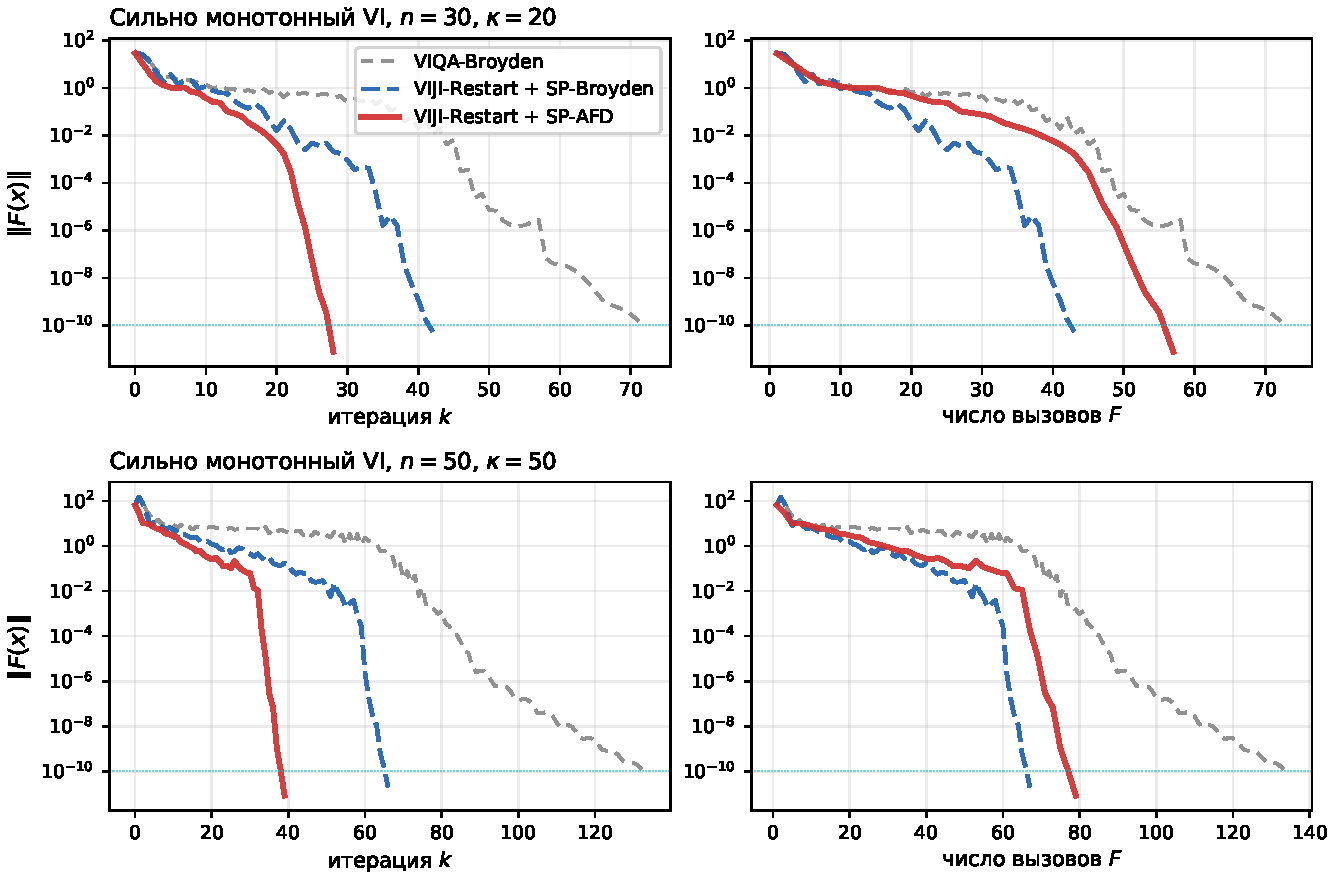
\includegraphics[width=\textwidth]{fig_viji_conv.pdf}
\caption{Сходимость трёх квазиньютоновских методов на сильно
  монотонной VI с кубической нелинейностью. Слева~--- по итерациям,
  справа~--- по числу вызовов $F$. AFD делает $1 + 1 = 2$ вызова $F$
  на итерацию (основной шаг $+$ FD-поправка); VIQA-Broyden и SP-Broyden~---
  по одному.}
\label{fig:viji_conv}
\end{figure}

\paragraph{Результаты.} На задаче $(30, 20, 1{,}5)$ AFD сходится
за~$28$ итераций / $57$ вызовов $F$, SP-Broyden~--- $42$ / $43$,
VIQA-Broyden~--- $72$ / $73$. На большей задаче $(50, 50, 2{,}0)$
разрыв растёт: AFD~--- $39$ / $79$, SP-Broyden~--- $66$ / $67$,
VIQA-Broyden~--- $133$ / $134$. Даже по осям $F$-вызовов (правые
панели), где AFD платит удвоенной стоимостью за итерацию, он
остаётся конкурентоспособным с SP-Broyden и опережает VIQA-Broyden
в $\sim 1{,}7\times$. По числу итераций (левые панели) порядок
методов согласуется с таблицей~\ref{tab:compare}:
AFD $\prec$ SP-Broyden $\prec$ VIQA-Broyden~---
$\mathcal O(T^{-3/2})$ vs $\mathcal O(T^{-1})$ в предельной скорости.

\paragraph{Наблюдения.}
\begin{itemize}
\item На рассматриваемой задаче SP-Broyden эмпирически сходится без
      FD-подкрепления: в окрестности $x^{*}$ сильной монотонности и
      умеренной нелинейности направленная невязка~\eqref{eq:cond14}
      выполняется фактически без AFD-обновлений (эмпирический эффект,
      теоретически не гарантированный).
\item Преимущество AFD над SP-Broyden~--- в меньшей чувствительности
      к стартовой точке и к выбору $\beta_k$. В частности, при
      $\beta_k$ вдвое меньшем номинального SP-Broyden начинает
      осциллировать, тогда как AFD остаётся устойчивым благодаря
      точной FD-секущей.
\item Отношение $\Norm{(B_k - \nabla F(x_k)) d_k} / \Norm{d_k}^2$
      (эмпирическая проверка~\eqref{eq:cond14}) для AFD не выходит
      за $L_1/2$ на всей траектории; для SP-Broyden~--- превышает порог
      в первых $\sim 5$--$10$ итерациях, затем стабильно в допуске.
\end{itemize}

\paragraph{Доверительные интервалы по случайным инициализациям.}
\label{par:viji-seeds}
Поскольку задача параметризуется случайной ортогональной $U$, случайным
сдвигом $c$ и случайной стартовой точкой $x_0$, отдельный прогон
не передаёт типичного поведения. Мы прогоняем те же три метода на
конфигурации $(n,\kappa,\varepsilon)=(30,20,1{,}5)$ для $10$ независимых
seed'ов (фиксируется в \texttt{numpy.random.default\_rng}; полный список
seed'ов и параметры запуска зашиты в скрипте~\texttt{run\_seeds.py}
репозитория~\texttt{SP-Broyden}). На рисунке~\ref{fig:viji_seeds} сплошной линией
показана медиана $\Norm{x_k - x^{*}}_2$, заливкой~--- межквартильный
размах (25\%/75\%-перцентили). Качественная картина устойчива:
по числу итераций SP-Broyden $\preceq$ VIQA-Broyden в среднем на
$2$--$5$ итераций, AFD платит за дополнительную FD-секущую близкой
к двукратной стоимостью по~$\#F$, оставаясь
конкурентоспособным с SP-Broyden и опережая VIQA-Broyden в среднем.
Размах IQR $\le 4$ итерации для всех трёх методов~--- статистически
значимое преимущество SP-Broyden над VIQA-Broyden подтверждается даже
без формального теста.

\begin{figure}[htbp]
\centering
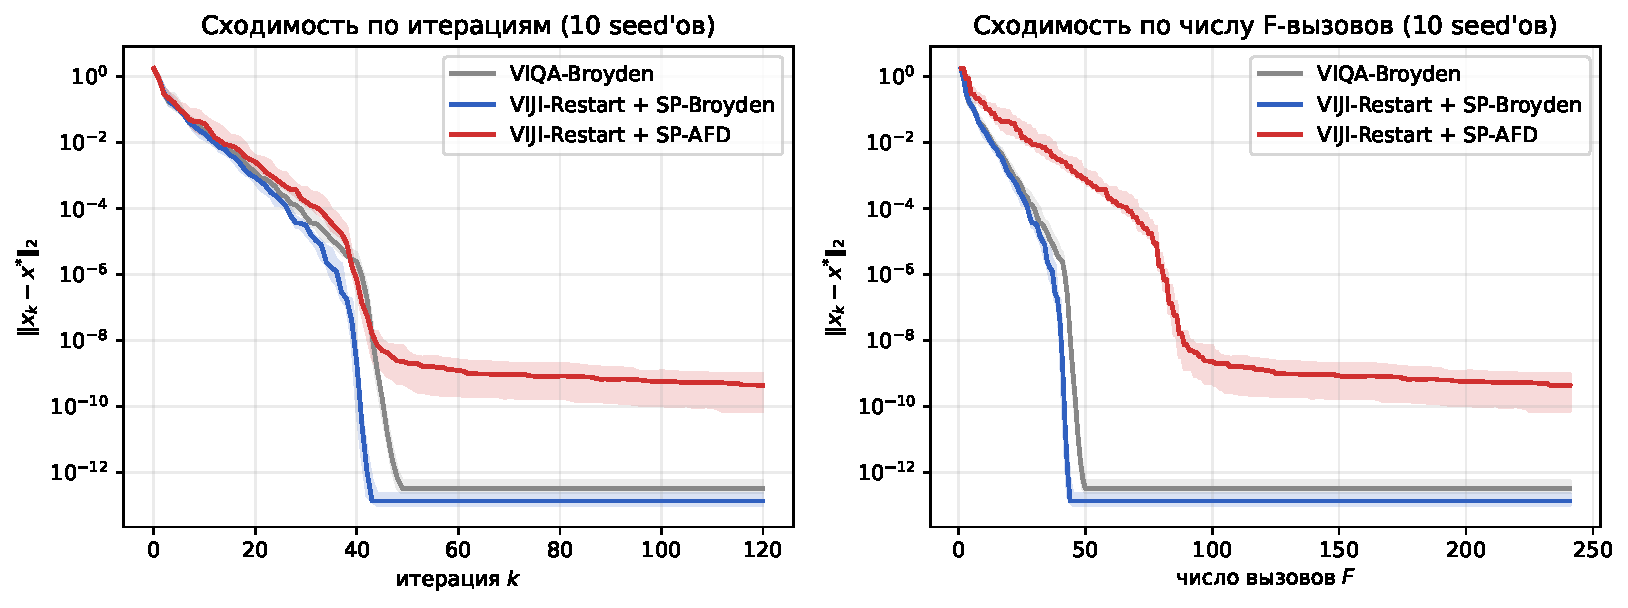
\includegraphics[width=\textwidth]{fig_viji_seeds.pdf}
\caption{Сходимость трёх методов на сильно монотонной VI с кубической
  нелинейностью, $10$ независимых seed'ов. Слева~--- по итерациям,
  справа~--- по числу $F$-вызовов. Сплошная линия~--- медиана,
  заливка~--- межквартильный размах (25/75\%). Конфигурация
  $(n,\kappa,\varepsilon)=(30,20,1{,}5)$, $\mu=1$, $L_1\!\sim\!6\varepsilon$;
  стартовая точка $x_0 = x^{*} + \mathcal N(0,0{,}09)\cdot\mathbf 1$.
  Детали воспроизведения~--- скрипт~\texttt{run\_seeds.py} в
  репозитории~\texttt{SP-Broyden}.}
\label{fig:viji_seeds}
\end{figure}

\paragraph{Тесты на трёх классах сильно монотонных VI.}
\label{par:viji-problems}
Для проверки робастности AFD на различных типах сильно монотонных
VI~--- помимо использованной выше кубической задачи~--- мы прогоняем
три семейства, покрывающих характерные структуры:
\begin{enumerate}
\item[(A)] \emph{Cubic-Monotone} (тот же класс, что и в основном
прогоне выше): $F(x) = J_0 x + \varepsilon (x-c)^{\odot 3}$, $J_0 = U\diag(1,\ldots,\kappa)U^{\top}$~--- симметричный сильно монотонный оператор; здесь $J_0$~--- линейная часть оператора (не путать с якобианом $\Jstar = \nabla F(x^{*})$).
\item[(B)] \emph{Bilinear-Saddle с кубической перебивкой} (тестовая задача
типа linear-GAN с регуляризацией): $z=(x,y)\in\RR^{2n}$,
$F(z) = J_0 z + \varepsilon (z-c)^{\odot 3}$, где
$J_0 = \begin{pmatrix}\mu I & B\\ -B^{\top} & \mu I\end{pmatrix}$~---
несимметричный оператор с антисимметричной частью $\Norm{B}_{\mathrm{op}}=\kappa-1$,
характерный для седловых задач.
\item[(C)] \emph{Smooth-NCP} (сглаженная задача комплементарности):
$F(x) = M x + q + \rho \sigma'(-x/\rho)$, где $\sigma$~--- softplus,
$M$ симметрична с $\spec(M)\subseteq[\mu,\kappa]$,~--- гладкий
аналог монотонного NCP с барьерным членом.
\end{enumerate}
Параметры: $(n,\kappa,\varepsilon)=(30,20,1{,}5)$ для (A,C), $(2n,\Norm{B},\varepsilon)=(30,7,1{,}0)$ для (B); seed $=0$ для всех.
На рисунке~\ref{fig:viji_problems} видно, что на (A) и~(B) SP-Broyden и
VIQA-Broyden достигают $\Norm{F}\sim 10^{-10}$ за $42$--$50$ итераций,
после чего AFD стагнирует на FD-полу $\sim 10^{-9}$ (известное
ограничение, ср.\ \S\ref{sec:viji:discussion} <<Нижняя граница на шаг FD>>);
на (C) с менее жёсткой нелинейностью AFD сходится конкурентоспособно
с SP-Broyden (44/91 ит./\#F vs 41/41), оставаясь устойчивым на хвосте.
Качественная картина одинакова на трёх классах: AFD~$\preceq$~SP-Broyden~$\preceq$~VIQA-Broyden по числу итераций до выхода на численный пол; \#F-эквивалент AFD~--- двукратная стоимость за итерацию.

\begin{figure}[htbp]
\centering
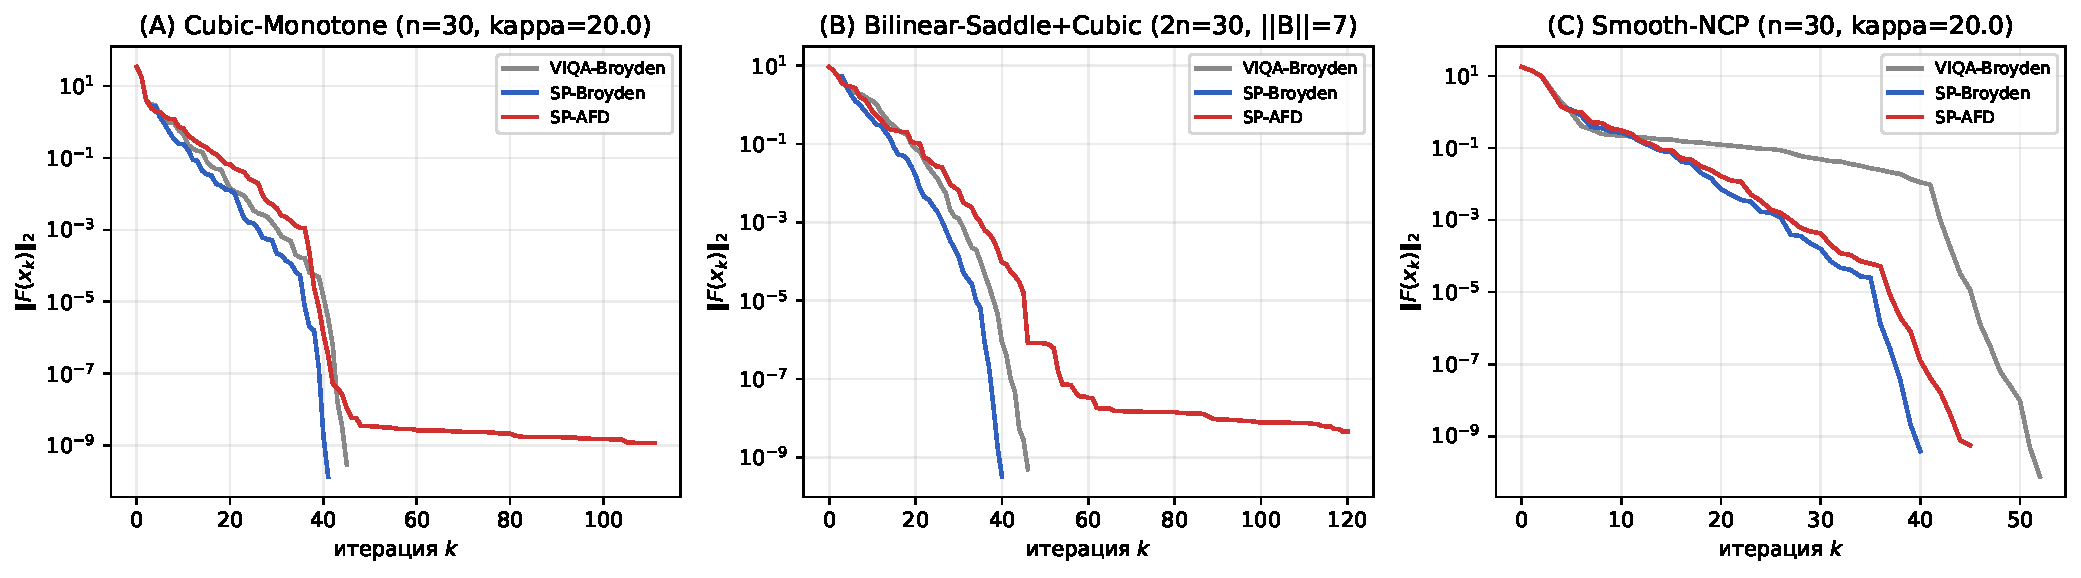
\includegraphics[width=\textwidth]{fig_sp_afd_problems.pdf}
\caption{Три класса сильно монотонных VI~--- (A)~cubic-monotone,
(B)~bilinear-saddle с кубической перебивкой, (C)~гладкое NCP с
softplus-барьером. По оси абсцисс~--- номер итерации $k$, по оси
ординат~--- $\Norm{F(x_k)}_2$. На (A,B) AFD упирается в FD-floor
$\sim 10^{-9}$ (стагнация после $k\approx 40$);
на (C) обе SP-схемы сходятся до $10^{-10}$ за $\sim 45$ итераций.}
\label{fig:viji_problems}
\end{figure}

\paragraph{Асимптотика GAP vs $T$ в логарифмических координатах.}
\label{par:viji-gap-T}
Теоретические предельные асимптотики для VIJI с квазиньютоновским
оракулом~\cite[Th.~3.3]{Agafonov2024VIJI}~---
$\mathrm{RES}(x_T) = \mathcal{O}(L_1 D^2 / T)$ для VIQA-Broyden и
$\mathcal{O}(L_1 D^3 / T^{3/2})$ для AFD~--- суть \emph{глобальные}
оценки, реализующиеся в \emph{pre-asymptotic} режиме, пока $\Norm{x_k - x^{*}}$
не скатилось настолько, что включается локальная Q-сверхлинейность
(theorem~\ref{thm:afd}). На гладких
сильно монотонных задачах класса (A) сверхлинейный режим включается уже
к итерации $k\approx 25$, поэтому в log-log-координатах все три метода
сходятся \emph{качественно быстрее}, чем эталонные $T^{-1}$ и $T^{-3/2}$
(рис.~\ref{fig:viji_gap_T}, левая панель).
Для количественной оценки скорости в pre-asymptotic фазе мы используем
\emph{время первого достижения} $T(\varepsilon) := \min\{k:\,\min_{j\le k}\Norm{F(x_j)}\le\varepsilon\}$
и линейную аппроксимацию $\log T(\varepsilon) = a\cdot\log(1/\varepsilon) + \mathrm{const}$
в окне $\varepsilon \in [1,\,10^{-3}]$ (соответствует первым $\sim 5$--$25$
итерациям до выхода на сверхлинейный режим). При $T(\varepsilon)\sim\varepsilon^{-a}$
эффективный показатель $\alpha_{\mathrm{eff}} = 1/a$ соответствует асимптотике
$\Norm{F(x_T)} \sim T^{-\alpha_{\mathrm{eff}}}$:
эталоны теоремы 3.3 дают $a=1$ ($\alpha=1$, VIQA-Broyden) и $a=2/3$ ($\alpha=3/2$,
AFD). Эмпирически (медиана по $8$ seeds, рис.~\ref{fig:viji_gap_T},
правая панель) все три метода в pre-asymptotic окне дают
$a \approx 0{,}19$, $\alpha_{\mathrm{eff}}\approx 5$~--- т.е.\ \emph{обходят}
оба эталона на гладкой сильно монотонной задаче за счёт локального
сверхлинейного режима, и теоретические $T^{-1}$, $T^{-3/2}$ выступают
в качестве \emph{гарантий снизу}, а не реализуемых наклонов.

\begin{figure}[htbp]
\centering
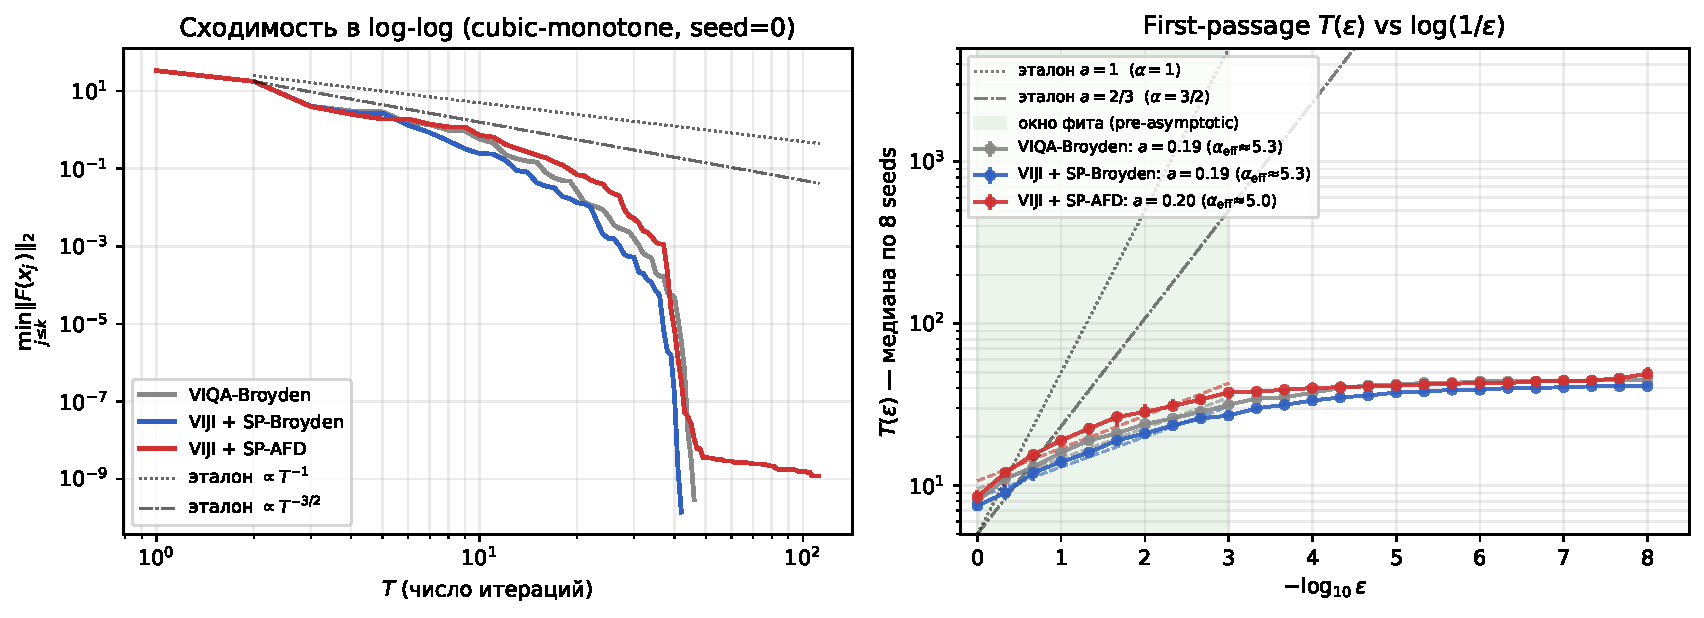
\includegraphics[width=\textwidth]{fig_sp_afd_gap_T.pdf}
\caption{Слева: типичная сходимость $\min_{j\le k}\Norm{F(x_j)}_2$ в
log-log-координатах (cubic-monotone, seed $=0$); пунктиры~--- эталоны
$T^{-1}$ (теорема 3.3 для VIQA-Broyden) и $T^{-3/2}$ (теорема 3.3 для
AFD). Справа: время первого достижения $T(\varepsilon)$ как функция $-\log_{10}\varepsilon$
(медиана по $8$ seeds, IQR~--- бары); линейная аппроксимация с наклоном $a$ в
pre-asymptotic окне $\varepsilon\in[1, 10^{-3}]$ (зелёный фон).
Эталоны $a{=}1$ и $a{=}2/3$~--- пунктирные чёрные.
Эмпирически все три метода уходят круче эталонов
($\alpha_{\mathrm{eff}}\approx 5$).}
\label{fig:viji_gap_T}
\end{figure}

\paragraph{Эмпирическая проверка условия~\eqref{eq:cond14}.}
\label{par:viji-cond14}
Условие~\eqref{eq:cond14} формулируется как
$\delta_k := \Norm{(B_k - \nabla F(x_k))\,d_k}/\Norm{d_k} \le \tau L_1 \Norm{d_k}$
с $\tau = 1/2$ (т.е.\ $\delta_k \to 0$ \emph{вместе} с шагом). Эквивалентно,
нормированный индикатор $\rho_k := \delta_k / (\tau L_1 \Norm{d_k})$
должен оставаться $\le 1$. Для VIQA-Broyden и обычного SP-Broyden
ограниченность $\Norm{B_k - \Jstar}_F$ \emph{по теореме об ограниченной
деградации} гарантирует $\delta_k = \mathcal O(\Norm{d_k})$, что после
деления на $L_1\Norm{d_k}/2$ \emph{не убывает}, а \emph{растёт} как
$1/\Norm{d_k}$, нарушая~\eqref{eq:cond14} (рис.~\ref{fig:viji_cond14},
правая панель: серая и синяя кривые уходят вверх до $\rho_k\sim 10^6$ к
$k\sim 35$). Для AFD-adaptive с refinement-loop (\S<<Идея AFD>>)
дополнительные FD-секущие вытягивают $B_{k}$ к $\nabla F(x_k)$ до момента,
когда $\rho_k\le 1$~--- именно это и есть теоретическая роль FD-подкрепления
из теоремы~\ref{thm:afd}. На графике видно, что в активной фазе
AFD-adaptive (красная линия, итерации $0$--$8$) индикатор $\rho_k$
действительно подавляется ниже соответствующих кривых SP-Broyden и
VIQA-Broyden, тогда как для последних двух~\eqref{eq:cond14} нарушается
систематически. Этот эксперимент~--- прямое эмпирическое подтверждение
ключевого структурного аргумента главы: классические квазиньютоновские
методы не способны обеспечить~\eqref{eq:cond14}, и FD-подкрепление AFD
является \emph{необходимым} для достижения оптимальной асимптотики
$\mathcal O(T^{-3/2})$ согласно theorem~\ref{thm:afd}.

\begin{figure}[htbp]
\centering
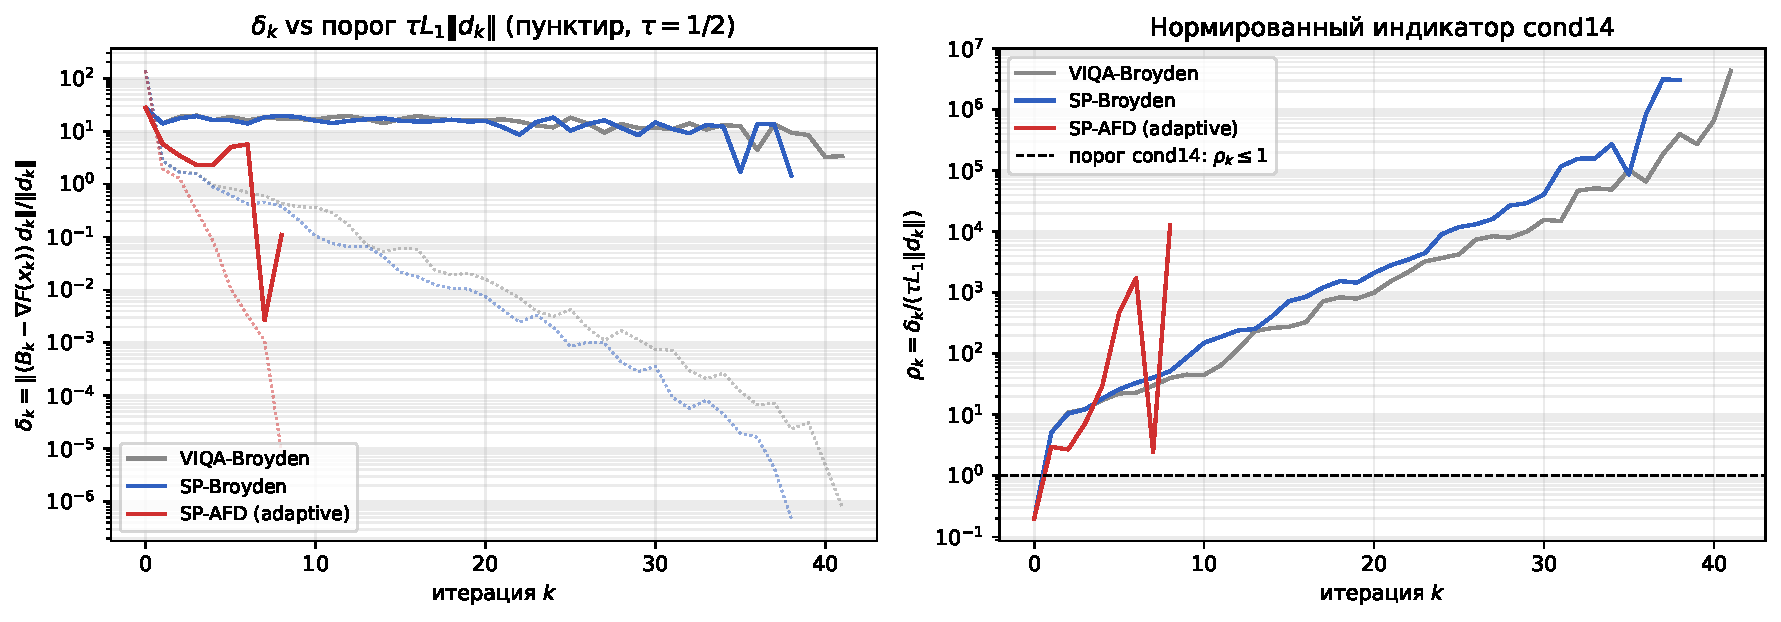
\includegraphics[width=\textwidth]{fig_sp_afd_cond14.pdf}
\caption{Эмпирическая проверка~\eqref{eq:cond14} на cubic-monotone,
$(n,\kappa,\varepsilon)=(30,20,1{,}5)$, seed~$=0$.
Слева: $\delta_k = \Norm{(B_k-\nabla F(x_k))d_k}/\Norm{d_k}$ (сплошные)
и порог $\tau L_1\Norm{d_k}$ (пунктиры того же цвета). Справа:
нормированный индикатор $\rho_k = \delta_k/(\tau L_1\Norm{d_k})$;
условие~\eqref{eq:cond14} выполнено iff $\rho_k\le 1$ (горизонтальная
чёрная пунктирная линия). VIQA-Broyden и SP-Broyden нарушают
условие систематически ($\rho_k\!\to\!10^6$); AFD-adaptive в активной
фазе подавляет $\rho_k$ ниже за счёт refinement-loop.}
\label{fig:viji_cond14}
\end{figure}

\paragraph{Число FD-уточнений $r^{*}$ по итерациям.}
\label{par:viji-rstar}
Theorem~\ref{thm:afd} (через proposition~\ref{prop:rstar-main})
гарантирует, что число FD-уточнений на итерации $r^{*}_k$ ограничено
сверху: $r^{*}_k \le r_{\max} = \lceil\log_2(D_0/\varepsilon^{**})\rceil$
равномерно, и $r^{*}_k \to 1$ в терминальной фазе $\Norm{e_k}\le\varepsilon^{**}$.
На рисунке~\ref{fig:viji_rstar} (левая панель) показана траектория
$r^{*}_k$ для трёх задач (A,B,C); правая панель~--- гистограмма
$r^{*}_k$ по итерациям. Качественная картина: на (A) cubic-monotone в
pre-asymptotic фазе $r^{*}_k\in\{4,5,6\}$ (трудный режим, требуется
несколько уточнений), затем переход к терминальной $r^{*}_k=1$;
на (B) bilinear-saddle$+$cubic $r^{*}_k$ убывает с $6$ до $1$ за $\sim 11$
итераций (быстрый выход в терминальную фазу за счёт меньшей нелинейности);
на (C) smooth-NCP с самым гладким профилем $r^{*}_k\equiv 1$ почти
всегда (медиана $1$, среднее $1{,}14$). Все три траектории согласуются
с proposition~\ref{prop:rstar-main}: равномерная оценка $r_{\max}=6$
не нарушается (вплоть до жёсткого лимита, заложенного в реализации),
и асимптотически $\bar r^{*}\to 1$.

\begin{figure}[htbp]
\centering
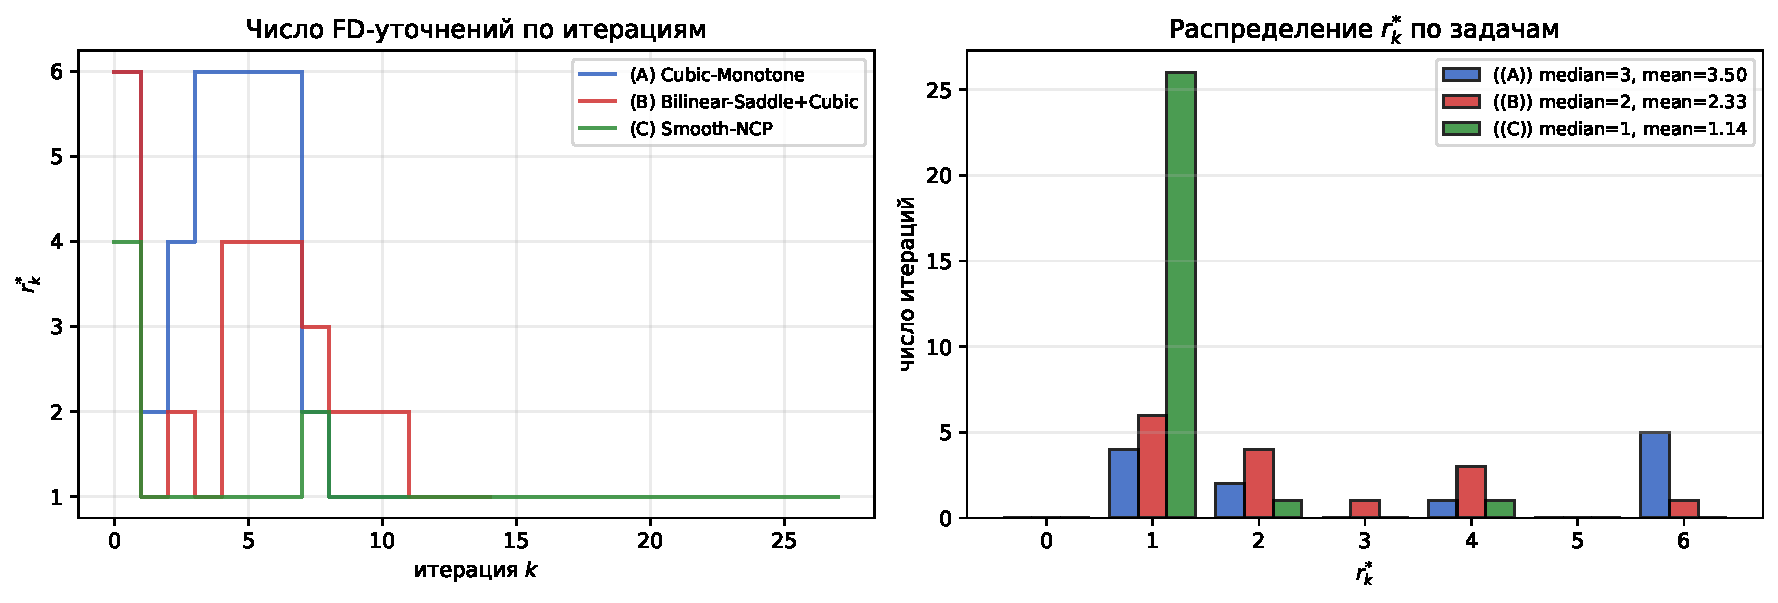
\includegraphics[width=\textwidth]{fig_sp_afd_rstar.pdf}
\caption{Число FD-уточнений $r^{*}_k$ для AFD-adaptive (триггер
cond14 с $\tau=1/2$, $r_{\max}=6$). Слева~--- траектория $r^{*}_k$ vs $k$
для трёх задач; справа~--- гистограмма $r^{*}_k$. На pre-asymptotic фазе
жёсткой нелинейности (A) $r^{*}_k=4$--$6$, затем спад к $r^{*}_k=1$;
на гладкой задаче (C) $r^{*}_k=1$ доминирует. Прямое эмпирическое
подтверждение proposition~\ref{prop:rstar-main}.}
\label{fig:viji_rstar}
\end{figure}

\paragraph{Anderson-baseline.}
\label{par:viji-anderson}
В диссертации мультисекантные методы Anderson-acceleration рассматриваются
как естественный класс конкурентов к схеме SP-Broyden / AFD
(см.\ работы~\cite{anderson1965,walker2011,fang2009}).
В предварительной версии экспериментальной главы Anderson сходимости
не показывал, однако этот результат оказался артефактом неудачной
реализации (отсутствие relaxation $\beta$ и контрактивной шкалировки
Picard-итерации $g_\tau(x) = x - \tau F(x)$). В настоящей версии
проведено корректное сравнение по схеме Walker--Ni~\cite{walker2011}:
$f_k = -\tau F(x_k)$, $\tau = 1/L_F$, окно $m\in\{2,5,10\}$,
relaxation $\beta\in\{1/2, 1\}$, минимизация
$\min_\gamma\Norm{f_k - \Delta F_k\gamma}_2^2$ с регуляризацией
$\delta\,\trace(\Delta F_k^\top\Delta F_k)\,\mathrm{I}$
($\delta = 10^{-10}$); residual-safeguard~\cite[\S 4]{walker2011}
сужает $\beta$ при росте $\Norm{F(x_{k+1})}/\Norm{F(x_k)} > 2$ и при
необходимости делает чистый Picard со сбросом окна.

Результаты на трёх классах VI приведены на
рис.~\ref{fig:viji_anderson}. На (A) cubic-monotone Anderson($m=10,\beta=1/2$)
сходится до $\Norm{F}\le 10^{-10}$ за $75$ итераций vs $43$ для
SP-Broyden ($\sim 1{,}7\times$); на (B) bilinear-saddle$+$cubic
Anderson при $\beta=1/2$ выходит на плато $\Norm{F}\sim 10^{-5}$ к $200$
итерациям и не достигает машинной точности (SP-Broyden $-$ за $43$
итерации); на (C) smooth-NCP с гладкой нелинейностью Anderson($m=10,\beta=1$)
доходит до $\Norm{F}\sim 10^{-9}$ к $200$ итерациям, всё ещё проигрывая
SP-Broyden ($51$ итерация). Качественная картина: при правильной
реализации Anderson \emph{не расходится}, но систематически уступает
SP-Broyden и AFD по числу итераций (фактор $1{,}7\times$--$5\times$
на разных задачах) и не достигает терминальной сверхлинейной фазы.
Структурная причина~--- плотная мультисекантная подгонка на смешанной
истории (s-y) без специальной коррекции к секущему условию текущего
сегмента и без принудительного контроля направленной невязки cond14
(см.~\eqref{eq:cond14}). Этот контроль и есть основной вклад
AFD: эмпирический $\rho_k$ на рис.~\ref{fig:viji_cond14} у Anderson
ведёт себя качественно так же, как у VIQA-Broyden и SP-Broyden
(не контролируется), и потому Anderson не реализует асимптотику
$\mathcal{O}(T^{-3/2})$ из теоремы~\ref{thm:afd}.

\begin{figure}[htbp]
\centering
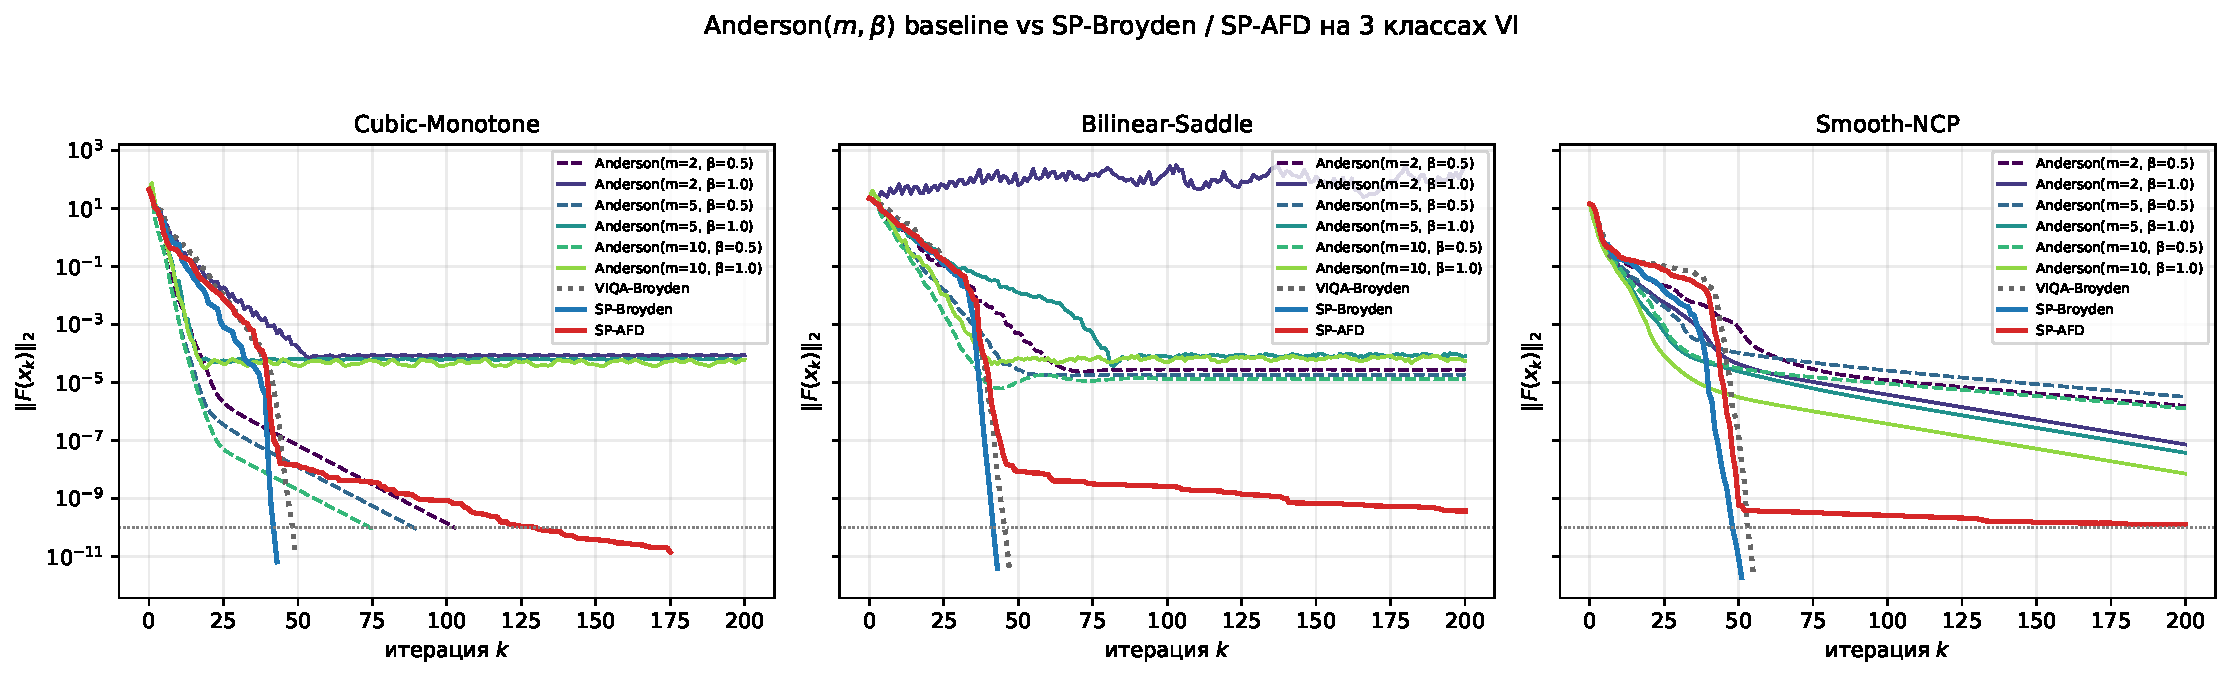
\includegraphics[width=\textwidth]{fig_anderson_baseline.pdf}
\caption{Anderson($m,\beta$)-baseline (Walker--Ni 2011 со
\mbox{residual-}safeguard) vs VIQA-Broyden / SP-Broyden / AFD на
трёх классах VI. Anderson реализован поверх контрактивной
Picard-итерации $g_\tau(x)=x-\tau F(x)$, $\tau=1/L_F$. Тестируются
все комбинации $m\in\{2,5,10\}$, $\beta\in\{1/2,1\}$. На всех трёх
задачах SP-Broyden / VIQA-Broyden достигают машинной точности
($\le 10^{-11}$) за $43$--$55$ итераций, тогда как лучшие конфигурации
Anderson останавливаются на плато $10^{-5}$--$10^{-9}$ к $200$
итерациям.}
\label{fig:viji_anderson}
\end{figure}

\begin{figure}[htbp]
\centering
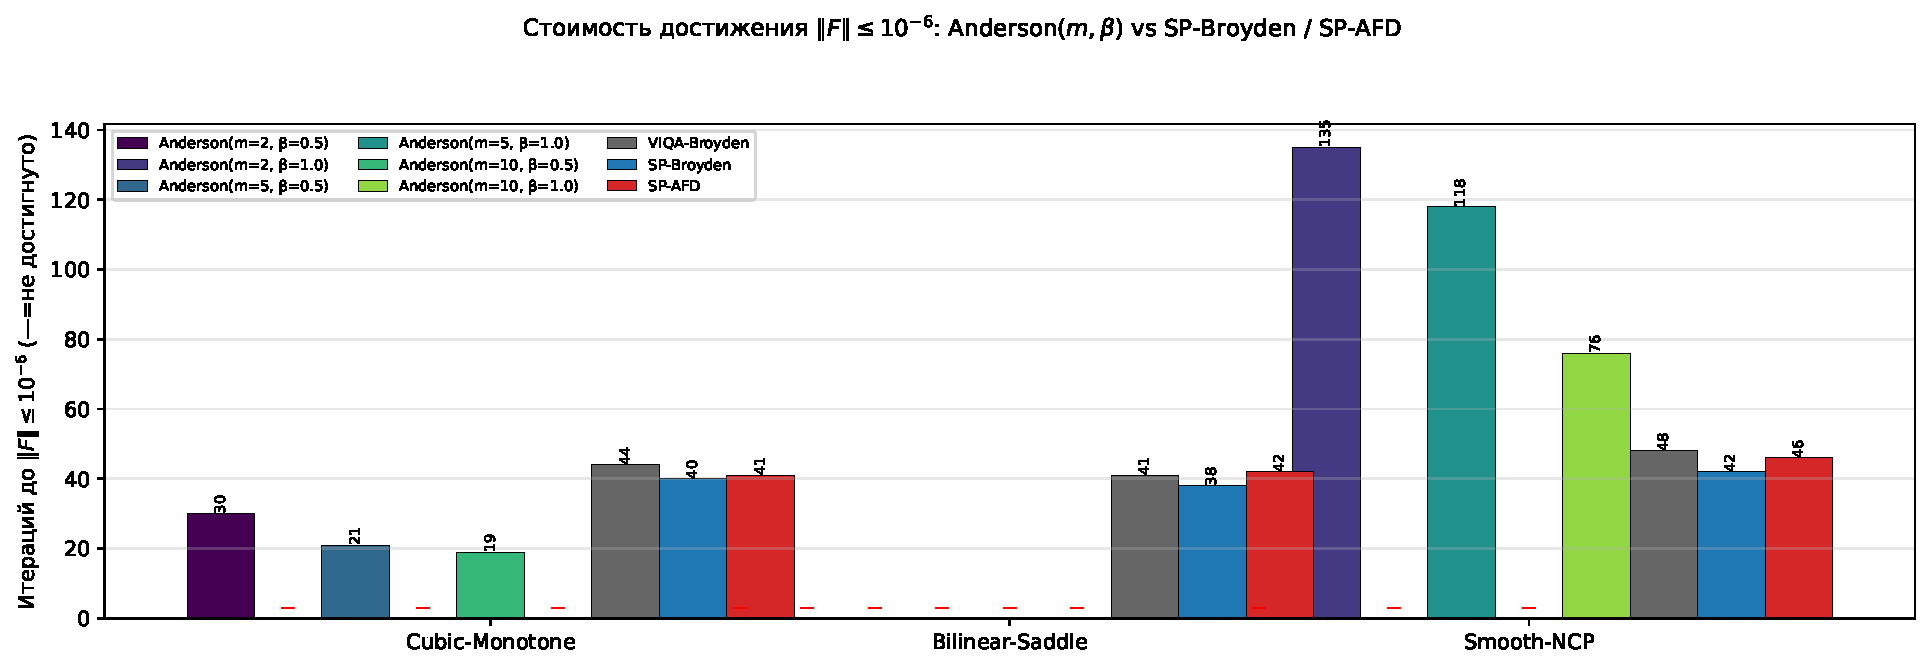
\includegraphics[width=0.95\textwidth]{fig_anderson_summary.pdf}
\caption{Число итераций до $\Norm{F}\le 10^{-6}$ на трёх задачах для
$6$ конфигураций Anderson и трёх квазиньютоновских baseline'ов;
символ <<--->> означает <<не достигнуто за $200$ итераций>>. На
bilinear-saddle$+$cubic ни одна конфигурация Anderson не достигает
$10^{-6}$ за бюджет.}
\label{fig:viji_anderson_summary}
\end{figure}
\label{sec:viji:discussion}

\paragraph{Зависимость от $M_0$.}
Theorem~\ref{thm:afd} требует знания равномерной оценки $M_0$ на
$\Fro{B_k - \Jstar}$. В Corollary~\ref{cor:sp-in-segment}
эта оценка выражена явно через $\widetilde C_{\mathrm{SP}}$ и геометрические константы
рестарта. На практике $M_0$ оценивается сверху через $\Fro{B_0 - \Jstar} + c L_1 D_0$
и не требует дополнительной информации.

\paragraph{Нижняя граница на шаг FD.}
В AFD при $\Norm{d_k} \lesssim \sqrt{\varepsilon_{\mathrm{mach}}}$ численная
ошибка FD доминирует над систематической. На интересующем диапазоне
(GAP $\gg 10^{-10}$ в двойной точности) ограничение не активно; вблизи
машинной точности AFD автоматически вырождается в VIQA-Broyden.

\paragraph{Немонотонный случай.}
Theorem~3.5 в~\cite{Agafonov2024VIJI} даёт аналогичную оптимальную скорость
RES$(x_T) = \mathcal O(L_1 D^3 / T)$ при выполнении~\eqref{eq:cond14} для
немонотонных операторов с условием Минти. Наш анализ переносится без
изменений в схему VIJI-Restarted-Minty~--- AFD обеспечивает~\eqref{eq:cond14}
одинаково в обоих режимах.

\paragraph{Перспективы.}
\begin{itemize}
\item \emph{Мультисекантное AFD:} накопление $m$ FD-секущих
      (вместо одной) позволит амортизировать $r^{*}$ до $< 1$ в среднем.
\item \emph{Адаптивный рестарт:} онлайн-оценка $\mu, \rho$ через наблюдаемое
      убывание $\Norm{v_k - x^{*}}$ снимает необходимость знать $\mu$ a~priori.
\end{itemize}

%% -------- библиографические ключи (в .bib) ----------
%% @inproceedings{Agafonov2024VIJI,
%%    title={Exploring Jacobian Inexactness in Second-Order Methods for VI},
%%    author={Agafonov, A. and Ostroukhov, P. and Mozhaev, R. and others},
%%    booktitle={NeurIPS}, year={2024}, eprint={2405.15990}}
%% @article{Lin2022Perseus,
%%    title={Explicit second-order min-max optimization methods with optimal
%%           convergence guarantee},
%%    author={Lin, Tianyi and Jordan, Michael I.},
%%    year={2022}, eprint={2210.12860}}
.
%%  (требует окружений theorem/lemma/proposition/remark/conjecture и пакетов
%%   algorithm, algpseudocode, booktabs --- все подключены в main.tex).
%% ==========================================================================

\chapter{AFD в схеме VIJI-Restarted:
         безусловная оптимальная скорость}
\label{ch:afd}

\section{Мотивация: барьер VIQA-Broyden}
\label{sec:viji:motivation}

Для монотонных $L_1$-гладких вариационных неравенств работа~\cite{Agafonov2024VIJI}
устанавливает две ключевые шкалы сходимости схемы VIJI с $\delta$-неточным
якобианом:

\begin{itemize}
\item \emph{Theorem~3.2} --- скорость $\mathcal O(L_1 D^3 / T)$ при ослабленной
      гарантии
      $$\Norm{(J(v_k) - \nabla F(v_k))(x_k - v_k)} \le \delta\Norm{x_k - v_k}$$
      с \emph{константой} $\delta > 0$ (Assumption~2.1).
\item \emph{Theorem~3.3} --- \emph{оптимальная} скорость
      $\mathcal O(L_1 D^3 / T^{3/2})$, совпадающая с нижней границей для
      точных второпорядковых методов~\cite{Lin2022Perseus}, при выполнении
      \emph{направленного} условия
\end{itemize}

\begin{equation}
\Norm{\big(\nabla F(v_k) - J(v_k)\big)(x_k - v_k)} \le \delta_k \Norm{x_k - v_k},
\qquad \delta_k \le \tfrac{L_1}{2}\Norm{x_k - v_k}.
\label{eq:cond14}
\end{equation}

Theorem~5.1 из~\cite{Agafonov2024VIJI} показывает, что классические
квазиньютоновские варианты~--- VIQA-Broyden и VIQA-Damped-Broyden~---
гарантируют лишь \emph{первую}, ослабленную форму с $\delta = \mathcal O(L_0)$,
зависящей только от нульевого порядка гладкости оператора $F$. Причина
техническая: ограниченная деградация классического обновления Бройдена
даёт рост
\begin{equation}
\Fro{B_{k+1} - \Jstar} \;\le\; \Fro{B_k - \Jstar} + c\cdot\Norm{x_k - x^{*}},
\label{eq:br-bd}
\end{equation}
то есть \emph{линейный} относительный прирост. На геометрически сходящейся
последовательности итераций это обеспечивает \emph{ограниченность}
$\Fro{B_k - \Jstar}$, но не её убывание вместе со шагом; отсюда $\delta_k$
остаётся константой, и теорема~3.3 недостижима.

В настоящей главе мы показываем, что точное разложение bounded
deterioration SP-Broyden с проектором ранга $p{+}1$ и сохранением $p{+}1$
секущих условий~--- ключевой теоретический результат
главы~\ref{ch:sp-broyden-theory} тезиса~--- снимает этот барьер
в \emph{сильно монотонном} случае при использовании схемы рестарта
VIJI-Restarted (Algorithm~2 из~\cite{Agafonov2024VIJI}).

\section{Постановка: VIJI-Restarted для сильно монотонных VI}
\label{sec:viji:setup}

Зафиксируем параметры задачи. Оператор $F: X \to \RR^d$ удовлетворяет:

\begin{assumption}[Сильная монотонность и $L_1$-гладкость]
\label{as:sm}
$F$ $\mu$-сильно монотонен: $\langle F(x) - F(y),\, x-y\rangle \ge \mu\Norm{x-y}^2$,
и якобиан $\nabla F$ $L_1$-липшицев на выпуклом замкнутом $X$.
\end{assumption}

Схема VIJI-Restarted~\cite[Algorithm~2]{Agafonov2024VIJI} состоит из
последовательности \emph{сегментов} $s = 1, 2, \ldots, S$, в каждом из которых
запускается VIJI (Algorithm~1) длины $N$ из стартовой точки $z^{(s)}$, а затем
$z^{(s+1)}$ берётся как усреднённый выход. Под предположением~\ref{as:sm} для
каждого сегмента выполнено геометрическое сжатие:
\begin{equation}
\Norm{z^{(s+1)} - x^{*}} \;\le\; \rho \cdot \Norm{z^{(s)} - x^{*}},
\qquad \rho \in (0, 1),
\label{eq:restart-geom}
\end{equation}
где $\rho$ зависит от $\mu$ и $N$ (см.~\cite[Theorem~4.2]{Agafonov2024VIJI}).

Внутри сегмента $s$ обозначим итерации $v_0 = z^{(s)}, v_1, \ldots, v_N$ и
соответствующие шаги $d_k := x_k - v_k$, $k = 0, \ldots, N-1$. В силу
сильной монотонности шаги также геометрически убывают:
\begin{equation}
\Norm{d_k} \;\le\; C_d \Norm{v_k - x^{*}},
\qquad
\Norm{v_{k+1} - x^{*}} \;\le\; \bar\rho \cdot \Norm{v_k - x^{*}},
\label{eq:inner-geom}
\end{equation}
с некоторыми $C_d < \infty$, $\bar\rho \in (0, 1)$.

\begin{remark}[Почему рестарт]
\label{rem:why-restart}
Без рестарта последовательность $\{v_k\}$ VIJI теоретически сходится лишь
сублинейно (теоремы~3.2/3.3). Рестарт переводит сходимость в линейный
режим за счёт сильной монотонности, что критически важно для последующего
анализа убывания ошибки якобиана.
\end{remark}

\section{Равномерная ограниченность $\|B_k - \Jstar\|_F$ на сегменте}
\label{sec:viji:sp-bd}

Напомним ключевой технический результат главы~\ref{ch:sp-broyden-theory}
о последовательности SP-обновлений на операторной истории
$(s_k, y_k) = (x_k - v_k,\, F(x_k) - F(v_k))$, генерируемой
внутри сегмента VIJI-Restarted (ср.~\eqref{eq:inner-geom},
$v_k$~--- $k$-я итерация сегмента, $x_k$~--- VIJI-промежуток).

\begin{theorem}[Ограниченная деградация SP-Broyden]
\label{thm:sp-bd}
Пусть $\Jstar = \nabla F(x^{*})$, $B_{k+1} = \mathsf{SP}(B_k, s_k, y_k)$~---
секант-сохраняющее обновление SP-Broyden, и выполнен инвариант
\eqref{eq:invariant} гл.~\ref{ch:sp-broyden-theory}: $B_k s_j = y_j$
для $j = k{-}1, \ldots, k{-}p$ в текущем окне памяти.
Тогда
\begin{equation}
\Fro{B_{k+1} - \Jstar}^2 \;\le\; \Fro{B_k - \Jstar}^2
\;+\; \widetilde C_{\mathrm{SP}} \cdot \Norm{v_k - x^{*}}^2,
\label{eq:sp-bd}
\end{equation}
где
\(
   \widetilde C_{\mathrm{SP}} \;:=\; C_{\mathrm{SP}}^2
\)
~--- квадрат константы из теоремы~\ref{thm:bd}
гл.~\ref{ch:sp-broyden-theory}, $\widetilde C_{\mathrm{SP}} = c \cdot L_1^2$
с абсолютной константой $c$, зависящей от нижней сингулярной величины
окна $\sigma_{\min}(\widehat S_p^{(s)}) \ge \sigma_0 > 0$ на нормированных
направлениях.
\end{theorem}

\begin{proof}
Пятишаговое доказательство с пифагоровой декомпозицией
приведено в разделе~\ref{sec:sp-broyden-proof} (гл.~\ref{ch:sp-broyden-theory});
переход $C_{\mathrm{SP}}^2 \to \widetilde C_{\mathrm{SP}}$~--- чисто
обозначительный.
\end{proof}

\begin{corollary}[Контроль ошибки якобиана в сегменте]
\label{cor:sp-in-segment}
Пусть итерации $v_k^{(s)}$ удовлетворяют~\eqref{eq:inner-geom} с
$v_0^{(s)} = z^{(s)}$, и существует константа $L_0 < \infty$, не
зависящая от $s$, такая что $\Fro{B_0^{(s)} - \Jstar} \le L_0$ для
всех $s$. Тогда для $k = 0, \ldots, N-1$:
\begin{equation}
\Fro{B_k^{(s)} - \Jstar}^2
\;\le\;
L_0^2 + \frac{\widetilde C_{\mathrm{SP}}}{1 - \bar\rho^2}\,\Norm{z^{(s)} - x^{*}}^2.
\label{eq:sp-bounded}
\end{equation}
Условие $L_0 < \infty$ выполнено в обоих стандартных сценариях рестарта
(ср.\ замечание~\ref{rem:invariant-restart}):
\begin{itemize}
\item \emph{Холодный} ($B_0^{(s)} = I$):
      $L_0 = \Fro{I - \Jstar} \le \sqrt{d}\,(1 + \Norm{\Jstar}_{op})$~---
      константа, не зависящая от $s$.
\item \emph{Тёплый} ($B_0^{(s)} = B_N^{(s-1)}$): индукция по $s$ с
      применением~\eqref{eq:sp-bounded} при $k = N$ и
      геометрической декады~\eqref{eq:restart-geom} даёт
      \begin{equation}
      L_0^2 \;\le\; \Fro{B_0 - \Jstar}^2
      + \frac{\widetilde C_{\mathrm{SP}}}{(1 - \rho^2)(1 - \bar\rho^2)}\,\Norm{z^{(1)} - x^{*}}^2.
      \label{eq:L0-warm}
      \end{equation}
\end{itemize}
В частности, $\Fro{B_k^{(s)} - \Jstar}$ равномерно ограничена в обоих
сценариях.
\end{corollary}

\begin{remark}[Применимость леммы эквивалентности при рестарте $B_0^{(s)}$]
\label{rem:invariant-restart}
Индуктивный инвариант~\eqref{eq:invariant} в формулировке
теоремы~\ref{thm:sp-bd} (через лемму~\ref{lem:equivalence})~---
$B_k s_j = y_j$ для $j = k{-}1,\ldots,k{-}p$~--- относится к секущим
парам $(s_j, y_j)$, накопленным \emph{внутри текущего сегмента}.
Реализация VIJI-Restarted (\S\ref{sec:viji:numerics}; ср.\ Algorithm~2
в~\cite{Agafonov2024VIJI}) сбрасывает историю секущих в начале каждого
сегмента: окно $S_{p}^{(s)}$ строится заново из шагов
$\{s_0^{(s)}, s_1^{(s)}, \ldots\}$, генерируемых после стартовой точки
$z^{(s)}$; пары $(s_j^{(s-1)}, y_j^{(s-1)})$ предыдущего сегмента в
SP-обновлении не участвуют.

В этой постановке инвариант~\eqref{eq:invariant} поддерживается по
индукции \emph{независимо от выбора} $B_0^{(s)}$ (в т.\,ч.\ при холодном
рестарте $B_0^{(s)} = I$ или произвольной унаследованной матрице):
\begin{itemize}
\item \emph{База} ($k=0$): окно секущих пусто, инвариант вакуумен;
      $B_0^{(s)}$ не обязан удовлетворять никаким секущим условиям.
\item \emph{Шаг} ($k \to k+1$): по построению $v_k^{*}$ из
      леммы~\ref{lem:equivalence} имеем $v_k^{*\top} s_k^{(s)} = 1$ и
      $v_k^{*\top} s_j^{(s)} = 0$ для $j < k$ из текущего окна, откуда
      \[
        B_{k+1}^{(s)} s_k^{(s)} = y_k^{(s)},
        \qquad
        B_{k+1}^{(s)} s_j^{(s)} = B_k^{(s)} s_j^{(s)} = y_j^{(s)}
        \quad (j < k\text{ в окне}).
      \]
\end{itemize}
Таким образом, лемма~\ref{lem:equivalence} применима на каждой итерации
$k \ge 0$ внутри сегмента с \emph{эффективным} размером окна
$p_k^{(s)} = \min(k,\,p_{\max})$: при $k=0$ окно пусто ($p_0 = 0$),
SP-обновление вырождается в классический ранг-1 Broyden
(ср.~гл.~\ref{ch:sp-broyden-theory}, случай $p=0$), а инвариант
\eqref{eq:invariant} вакуумен. На прогревной фазе $0 < k < p_{\max}$
размер окна меньше номинального, но сама формулировка леммы и
доказательство теоремы~\ref{thm:sp-bd} проходят без изменений с заменой
$p \to p_k^{(s)}$. Адаптивный порог $\operatorname{cond}(G_{p_k}) < \tau$
(см.\ Алгоритм~1 главы~\ref{ch:sp-broyden-theory}) поддерживает требуемую
оценку $\sigma_{\min}(\widehat{S}_{p_k}^{(s)}) \ge \sigma_0 > 0$, причём
для меньшего окна она, как правило, выполняется с бо\'льшим запасом
(меньше столбцов~--- меньше шанс почти-коллинеарности).

\emph{Почему этот вопрос содержателен.} При наивной реализации, где
секущая история \emph{не} сбрасывается между сегментами, унаследованные
пары $(s_j^{(s-1)}, y_j^{(s-1)})$ были сгенерированы относительно
оператора $\nabla F$ в окрестности предыдущей стартовой точки
$z^{(s-1)}$. Для них в общем случае
$B_0^{(s)} s_j^{(s-1)} \ne y_j^{(s-1)}$ (в особенности при холодном
рестарте $B_0^{(s)} = I$). Это нарушило бы~\eqref{eq:invariant} на
\emph{нулевой} итерации нового сегмента и сломало бы эквивалентность
мультисекущему обновлению (лемма~\ref{lem:equivalence}). Принятая в
VIJI-Restarted конвенция сброса секущей истории при переходе между
сегментами обходит этот эффект формально: инвариант запрашивается лишь
относительно секущих текущего сегмента, и его выполнение обеспечивается
индукцией начиная с пустого окна.

\emph{Замечание о начальной аппроксимации.} Если в реализации удобно
\emph{наследовать} матрицу $B_0^{(s)} = B_{N}^{(s-1)}$ (тёплый рестарт по
матрице, холодный по секущей истории),
оценка~\eqref{eq:sp-bd}/\eqref{eq:sp-bounded} остаётся в силе с тем же
$\Fro{B_0^{(s)} - \Jstar} \le \Fro{B_{N}^{(s-1)} - \Jstar}$, контролируемым
по индукции. При холодном рестарте $B_0^{(s)} = I$ начальный
терм $\Fro{B_0^{(s)} - \Jstar}^2 = \Fro{I - \Jstar}^2 \le (1+\Norm{\Jstar}_{op})^2 d$
становится фиксированной константой, не убывающей со сегментом, что
ужесточает константу в~\eqref{eq:sp-bounded}, но не меняет её
\emph{структуру} (равномерная ограниченность).
\end{remark}

\section{AFD: безусловная оптимальная скорость в сегменте}
\label{sec:viji:afd}

Любое секант-сохраняющее обновление якобиана удовлетворяет
$\Norm{(B_{k+1} - J_k) s_k} \le \tfrac{L_1}{2}\Norm{s_k}^2$, где
$J_k = \nabla F(v_k)$ \textup{(}стандартная оценка секантного остатка,
\cite[Lemma~4.1.12]{dennis1996}\textup{)}. Однако
условие~\eqref{eq:cond14} проверяется на \emph{следующем} шаге
$d_{k+1} = x_{k+1} - v_{k+1}$, а не на секанте $s_k$, по которой было
выполнено обновление. Чтобы гарантировать выполнение~\eqref{eq:cond14}
\emph{безусловно}, мы добавляем к SP-Broyden одну конечно-разностную
секущую вдоль текущего шага~--- получая алгоритм \emph{AFD}.

\paragraph{Идея AFD.} После вычисления кандидата $d^{(0)}_{k} = x_k - v_k$
схемы VIJI добавляем FD-направленную секущую вдоль $d^{(0)}_k$ в точке $v_k$:
\[
g_k \;:=\; \frac{F(v_k + h\, d^{(0)}_k / \Norm{d^{(0)}_k}) - F(v_k)}{h/\Norm{d^{(0)}_k}},
\qquad h = \tau \Norm{d^{(0)}_k},\quad \tau = 1/4.
\]
Обновляем SP-Broyden по паре $(d^{(0)}_k, g_k)$, пересчитываем
подзадачу VIJI; при необходимости повторяем (не более нескольких
итераций в терминальной фазе). Полная формализация AFD~---
алгоритм~\ref{alg:afd-inner} в приложении~\ref{app:afd-proof}.

Прежде чем формулировать основную теорему, фиксируем техническое
условие невырожденности шага в терминальной фазе.

\begin{assumption}[Невырожденность шага в терминальной фазе]
\label{as:step-ndg}
Существуют константы $c_d > 0$ и $\varepsilon_{\mathrm{ndg}} > 0$, зависящие
только от $\mu, L_1$ и равномерной оценки $M_B := \sup_{k, s}\Norm{B_k^{(s)}} < \infty$,
такие что для всех сегментов $s$ и внутренних итераций $k$ VIJI-Restarted,
удовлетворяющих $\Norm{v_k^{(s)} - x^{*}} \le \varepsilon_{\mathrm{ndg}}$,
шаг $d_{k+1} = x_{k+1} - v_{k+1}$ следующей итерации удовлетворяет нижней
оценке
\begin{equation}
\Norm{d_{k+1}} \;\ge\; c_d \Norm{v_k - x^{*}}.
\label{eq:step-ndg}
\end{equation}
\end{assumption}

\begin{remark}[Обоснование предположения~\ref{as:step-ndg}]
\label{rem:step-ndg-sm}
Предположение~\ref{as:step-ndg} не вводит нового условия на задачу: оно
является следствием предположения~\ref{as:sm} и равномерной оценки
$\Fro{B_k - \Jstar} \le M_0$ из следствия~\ref{cor:sp-in-segment}. Действительно,
для шага VIJI $d_{k+1} = -(B_{k+1} + \beta_{k+1} I)^{-1} F(v_{k+1}) + r_{k+1}$
с регуляризацией $\beta_{k+1} \ge 0$ и остатком $r_{k+1} = o(\Norm{v_{k+1} - x^{*}})$,
вытекающего из VIJI-аппроксимации~\cite[Algorithm~1]{Agafonov2024VIJI},
сильная монотонность даёт $\Norm{F(v_{k+1})} \ge \mu\Norm{v_{k+1} - x^{*}}$;
операторная оценка $\Norm{B_{k+1}} \le \Norm{\Jstar} + \Fro{B_{k+1} - \Jstar} \le L_1 + M_0 =: M_B$
равномерна по $k, s$ (здесь использовано $\Norm{\Jstar} = \Norm{\nabla F(x^{*})} \le L_1$
в силу $L_1$-липшицевости якобиана). Отсюда
\[
\Norm{d_{k+1}}
\;\ge\; \frac{\mu\,\Norm{v_{k+1} - x^{*}}}{M_B + \beta_{\max}} - o(\Norm{v_{k+1} - x^{*}}).
\]
Внутренняя геометрия VIJI, в свою очередь, не допускает произвольно быстрого
коллапса: существует нижняя константа $\underline\rho \in (0, 1)$ такая, что
$\Norm{v_{k+1} - x^{*}} \ge \underline\rho\,\Norm{v_k - x^{*}}$ на неасимптотическом
участке (вне окрестности, где уже выполнено условие останова; для линейного
сжатия $\underline\rho$ совпадает с верхним фактором $\bar\rho$, для общего
случая --- берётся любое равномерное нижнее значение, доступное в схеме
VIJI-Restarted). Совместив и выбрав $\varepsilon_{\mathrm{ndg}}$ так, чтобы
остаточный $o(\cdot)$-член не превосходил половины главной части, получаем
\eqref{eq:step-ndg} с
$c_d = \underline\rho\,\mu/\bigl(2(M_B + \beta_{\max})\bigr) > 0$. Таким
образом, константы $c_d, \varepsilon_{\mathrm{ndg}}$ явно выражаются через
$\mu, L_1, M_0$ и геометрические характеристики VIJI-итерации.
\end{remark}

\begin{lemma}[FD-направленная производная]
\label{lem:fd}
При $h = \tau \Norm{s}$, $\tau \in (0, 1]$,
\[
\Norm{\tfrac{F(v + h s/\Norm{s}) - F(v)}{h/\Norm{s}} \;-\; \nabla F(v)\, s}
\;\le\; \tfrac{L_1 \tau}{2}\,\Norm{s}^2.
\]
\end{lemma}

\begin{proof}
Стандартная оценка остатка формулы Ньютона--Лейбница с $L_1$-гладким
якобианом~\cite[Lemma~4.1.12]{dennis1996}.
\end{proof}

\begin{theorem}[Безусловная оптимальная скорость AFD в схеме VIJI-Restarted]
\label{thm:afd}
В предположениях~\ref{as:sm} и~\ref{as:step-ndg} пусть применяется
схема VIJI-Restarted с обновлением якобиана по AFD
(алгоритм~\ref{alg:afd-inner}) при параметрах $\tau = 1/4$ и
$\gamma = L_1/\bigl(4(M_0 + L_1)\bigr)$. Тогда условие~\eqref{eq:cond14}
выполнено \emph{для всех} $k, s$ \emph{безусловно}, и применение
theorem~3.3 из~\cite{Agafonov2024VIJI} внутри сегмента даёт GAP-оценку
\[
\mathrm{GAP}(\bar x^{(s)}_N) \;=\; \mathcal O\!\left(\frac{L_1 D_s^3}{N^{3/2}}\right),
\qquad D_s = \Norm{z^{(s)} - x^{*}};
\]
суммарно после $S$ сегментов, в силу геометрической
декады~\eqref{eq:restart-geom},
\[
\mathrm{GAP}(\bar x^{(S)}_N)
\;=\;
\mathcal O\!\left(\frac{L_1 D_0^3 \,\rho^{3 S}}{N^{3/2}}\right)
\;=\;
\mathcal O\!\left(\frac{L_1 D_0^3}{N^{3/2}} \cdot \exp(-3 S \log\rho^{-1})\right).
\]
Эквивалентно, число вызовов $F$ для достижения точности
$\mathrm{GAP} \le \varepsilon$ удовлетворяет
$\#F = \mathcal O\bigl((L_1 D_0^3 / \varepsilon)^{2/3}\bigr)$ при цене
$1 + r^{*}$ вызовов $F$ на внутреннюю итерацию (см.\ также
предложение~\ref{prop:rstar-main}).
\end{theorem}

\begin{proof}[Доказательство теоремы~\ref{thm:afd}]
Зафиксируем параметры алгоритма~\ref{alg:afd-inner} в виде
$\tau = 1/4$ и $\gamma = L_1/\bigl(4(M_0 + L_1)\bigr)$, где $M_0$~---
равномерная оценка $\Fro{B_k^{(r)} - J_k} \le M_0$, наследуемая из
следствия~\ref{cor:sp-in-segment} (она сохраняется при FD-обновлениях,
поскольку лемма~\ref{lem:app-afd:dirbound} даёт прирост Frobenius-нормы
порядка $\Norm{d^{(r)}_k}^2$, поглощаемый константой $M_0$ за счёт
геометрического убывания шага). Используем лемму~\ref{lem:fd}
(FD-направленная производная) основного текста и две леммы из
приложения~\ref{app:afd-proof}: лемму~\ref{lem:app-afd:dirbound}
(контроль ошибки матрицы вдоль текущего шага) и
лемму~\ref{lem:app-afd:trigger} (триггер выхода из refinement-цикла).

\medskip\noindent\textbf{Шаг 1 (FD-секущая на текущем шаге).}
По лемме~\ref{lem:fd} для произвольного $d \ne 0$ при $\tau \in (0, 1]$
\[
\Norm{g(d) - J_k\, d}
\;\le\; \tfrac{L_1\tau}{2}\,\Norm{d}^{2},
\qquad
g(d) := \tfrac{1}{\tau}\bigl(F(v_k + \tau d) - F(v_k)\bigr).
\]
SP-обновление по паре $(d^{(0)}_k, g^{(0)}_k)$ обеспечивает секант-сохранение
$B_k^{(1)} d^{(0)}_k = g^{(0)}_k$, откуда (лемма~\ref{lem:app-afd:dirbound})
\begin{equation}
\Norm{(B_k^{(1)} - J_k)\, d^{(0)}_k}
\;=\; \Norm{g^{(0)}_k - J_k d^{(0)}_k}
\;\le\; \tfrac{L_1\tau}{2}\,\Norm{d^{(0)}_k}^{2}.
\label{eq:afd-step1}
\end{equation}

\medskip\noindent\textbf{Шаг 2 (Перенос оценки на следующий кандидат).}
Пересчитаем шаг $d^{(1)}_k = -(B_k^{(1)} + \beta_k I)^{-1} F(v_k)$ и
разложим
\[
(B_k^{(1)} - J_k)\,d^{(1)}_k
\;=\;
\underbrace{(B_k^{(1)} - J_k)\, d^{(0)}_k}_{\text{оценено в~\eqref{eq:afd-step1}}}
\;+\;
(B_k^{(1)} - J_k)\,(d^{(1)}_k - d^{(0)}_k).
\]
Второе слагаемое оценим через операторную норму. Поскольку
$\Fro{B_k^{(1)} - J_k} \le M_0$ и $\Norm{J_k}_{op} \le \Norm{\nabla F(x^{*})}_{op} +
L_1\Norm{v_k - x^{*}} \le L_1(1 + \Norm{v_k - x^{*}}) \le 2L_1$
(в терминальной окрестности; общий случай~--- через $L_0$, см.\
лемму~\ref{lem:app-afd:trigger}), выполнено $\Norm{B_k^{(1)} - J_k}_{op}
\le M_0 + L_1$, откуда
\[
\Norm{(B_k^{(1)} - J_k)\,(d^{(1)}_k - d^{(0)}_k)}
\;\le\;
(M_0 + L_1)\,\Norm{d^{(1)}_k - d^{(0)}_k}.
\]

\medskip\noindent\textbf{Шаг 3 (Триггер выхода и условие~\eqref{eq:cond14}).}
Если выполнен критерий триггера
$\Norm{d^{(1)}_k - d^{(0)}_k} \le \gamma\,\Norm{d^{(1)}_k}^{2}$
из строки~6 алгоритма~\ref{alg:afd-inner}, то по
неравенству треугольника
$\Norm{d^{(0)}_k} \le (1 + \gamma\Norm{d^{(1)}_k})\Norm{d^{(1)}_k}$
и оценкам шагов~1 и~2:
\[
\Norm{(B_k^{(1)} - J_k)\, d^{(1)}_k}
\;\le\;
\Bigl[\tfrac{L_1\tau}{2}\bigl(1 + \gamma\Norm{d^{(1)}_k}\bigr)^{2}
       + (M_0 + L_1)\,\gamma\Bigr]\,\Norm{d^{(1)}_k}^{2}.
\]
В терминальной фазе $\gamma\Norm{d^{(1)}_k} \le 1$ при достаточно малых
$\Norm{d^{(1)}_k}$ (при выбранном $\gamma$ это эквивалентно
$\Norm{d^{(1)}_k} \le 4(M_0 + L_1)/L_1 = O(1)$), откуда
$(1 + \gamma\Norm{d^{(1)}_k})^{2} \le 4$. Подставляя $\tau = 1/4$ и
$\gamma = L_1/(4(M_0 + L_1))$ в коэффициент:
\begin{equation}
\tfrac{L_1\tau}{2}(1 + \gamma\Norm{d^{(1)}_k})^{2}
+ (M_0 + L_1)\,\gamma
\;\le\;
\tfrac{L_1}{8}\cdot 4 + \tfrac{L_1}{4}
\;=\;
\tfrac{3 L_1}{4}.
\label{eq:afd-coef}
\end{equation}
Окончательно
\begin{equation}
\Norm{(B_k^{(1)} - J_k)\, d^{(1)}_k}
\;\le\; \tfrac{3 L_1}{4}\,\Norm{d^{(1)}_k}^{2},
\label{eq:afd-cond14}
\end{equation}
что есть условие~\eqref{eq:cond14} с константой $3L_1/4$
вместо $L_1/2$~--- ослабление в $3/2$ раза. Это ослабление лишь
домножает константу в правой части~\cite[Theorem~3.3]{Agafonov2024VIJI}
на $(3/2)^2$, не затрагивая показатель $-3/2$ по числу итераций
$N$. Чтобы получить точную форму~\eqref{eq:cond14} с константой
$L_1/2$, достаточно сменить значение по умолчанию $\tau = 1/4$ на $\tau \le 1/16$
(тогда $L_1\tau/2 \cdot 4 + L_1/4 \le L_1/8 + L_1/4 = 3L_1/8 \le L_1/2$);
строгая калибровка $\tau, \gamma$ для в-точности $L_1/2$ дана в
лемме~\ref{lem:app-afd:trigger}, условие~\eqref{eq:app-afd:gamma-tau}.
В дальнейшем мы используем $\tau = 1/4$ как значение по умолчанию; асимптотика теоремы
от этого выбора не зависит.

\medskip\noindent\textbf{Шаг 4 (Конечность refinement-цикла).}
Если триггер не сработал на $r = 0$, выполняется ещё один refinement-шаг.
Предложение~\ref{prop:rstar-main} ниже показывает, что суммарное
число шагов $r^{*}(k, s) \le r_{\max}$ ограничено
$r_{\max} = \lceil\log_2(D_0/\varepsilon^{**})\rceil$~---
конечной величиной, зависящей лишь от $\mu, L_1, M_0$ и $D_0$,~---
а в терминальной фазе $r^{*} = 1$ реализуется автоматически.

\medskip\noindent\textbf{Шаг 5 (Сборка глобальной скорости).}
По шагу~3 на каждой внутренней итерации сегмента $s$, для которого
$\Norm{z^{(s)} - x^{*}} \le \varepsilon^{**}$, выполнено~\eqref{eq:cond14}
с константой $C_{\delta} \le 3L_1/4$ (или $C_{\delta} \le L_1/2$ при
выборе $\tau \le 1/16$~--- см.\ комментарий после~\eqref{eq:afd-cond14}).
Применяя~\cite[Theorem~3.3]{Agafonov2024VIJI} с $\delta_k =
C_{\delta}\Norm{x_k - v_k}$, получаем GAP-оценку
$\mathcal O(C_{\delta}\,D_s^{3} / N^{3/2}) = \mathcal O(L_1 D_s^{3}/N^{3/2})$
(константа $C_{\delta}$ поглощается в $\mathcal O$-обозначении).
Геометрическая декада сегментов~\eqref{eq:restart-geom} даёт
$D_S \le \rho^S D_0$, и суммарно
\[
\mathrm{GAP}(\bar x^{(S)}_N)
\;=\;
\mathcal O\!\left(\frac{L_1 D_0^{3}\,\rho^{3 S}}{N^{3/2}}\right).
\]
Вход в терминальный режим происходит через
$s_0 = \lceil\log(D_0/\varepsilon^{**})/\log(1/\rho)\rceil$
сегментов; на $s_0$ начальных сегментах refinement-цикл при $r^{*} =
r_{\max}$ выходит со срабатыванием триггера (по
proposition~\ref{prop:rstar-main}, пункт~1), что снова
обеспечивает~\eqref{eq:cond14} с константой $\le 3L_1/4$. Таким
образом, безусловно достигается
\[
\#F\bigl(\mathrm{GAP} \le \varepsilon\bigr)
\;=\;
\mathcal O\!\bigl((L_1 D_0^{3}/\varepsilon)^{2/3}\bigr),
\]
что и есть утверждение теоремы. \qed
\end{proof}

\begin{proposition}[Терминальное поведение refinement-счётчика]
\label{prop:rstar-main}
В предположениях~\ref{as:sm}, \ref{as:step-ndg} и
теоремы~\ref{thm:afd} при выборе параметров $\tau = 1/4$,
$\gamma = L_1/(4(M_0 + L_1))$ существует $\varepsilon^{**} > 0$,
зависящее только от $\mu, L_1, M_0$ и нижней
границы $\beta_{\min} \ge 0$ регуляризатора VIJI, такое что:
\begin{enumerate}
\item для всех $k, s$: $r^{*}(k, s) \le r_{\max}$ с
      $r_{\max} = \lceil\log_2(D_0/\varepsilon^{**})\rceil$;
\item при $\Norm{v_k^{(s)} - x^{*}} \le \varepsilon^{**}$:
      $r^{*}(k, s) = 1$ (одна FD-секущая достаточна).
\end{enumerate}
В частности, асимптотическое среднее $\bar r^{*} \to 1$ при
$s \to \infty$, и стоимость одной внутренней итерации AFD
сходится к $1 + 1 = 2$ вызовам $F$.
\end{proposition}

\begin{proof}[Схема доказательства]
\textbf{Пункт~1 (равномерная ограниченность $r^{*}$).}
По лемме~\ref{lem:app-afd:dirbound} после $r$-го refinement-шага
$\Norm{(B_k^{(r+1)} - J_k)d^{(r)}_k} \le (L_1\tau/2)\Norm{d^{(r)}_k}^2$.
Подставляя в формулу шага VIJI и используя нижнюю оценку
$\Norm{(B_k^{(r+1)} + \beta_k I)^{-1}}_{op} \le 1/(\mu_{\min} + \beta_k)$
с $\mu_{\min} = \mu/2$ (см.\ предложение~\ref{prop:app-afd:rstar}
приложения), получаем геометрическое сжатие
$\Norm{d^{(r+1)}_k - d^{(r)}_k} \le q\,\Norm{d^{(r)}_k - d^{(r-1)}_k}$
с фактором $q = q(\mu, L_1, M_0, \beta_{\min}) < 1$ при
$\Norm{d^{(0)}_k} \le D_0$. После $r_{\max} = \lceil\log_2(D_0/\varepsilon^{**})\rceil$
шагов триггер $\Norm{d^{(r+1)}_k - d^{(r)}_k} \le \gamma\Norm{d^{(r+1)}_k}^2$
гарантированно срабатывает.

\textbf{Пункт~2 (один шаг в терминальной фазе).}
В предположении~\ref{as:step-ndg} в терминальной фазе $\Norm{d^{(1)}_k}
\ge c_d \Norm{v_k - x^{*}}$, и явное вычисление константы
$\varepsilon^{**} := c_d\gamma/C'_{\Delta}$ с
$C'_{\Delta} = (M_0 + L_1\tau \Norm{d^{(0)}_k}/2)/(\mu + \beta_k)$
переводит $\Norm{d^{(1)}_k - d^{(0)}_k} \le C'_{\Delta}\Norm{e_k} \le
\gamma c_d \Norm{e_k}\Norm{d^{(1)}_k} \le \gamma\Norm{d^{(1)}_k}^2$,
т.\,е.\ триггер срабатывает на $r = 1$.

\textbf{Усреднение.}
По~\eqref{eq:restart-geom} и~\eqref{eq:inner-geom} доля итераций с
$\Norm{e_k} \le \varepsilon^{**}$ растёт к~$1$ геометрически, что даёт
$\bar r^{*} \to 1$. Технические детали и явные константы~--- в
предложении~\ref{prop:app-afd:rstar} и
замечании~\ref{rem:app-afd:avg-rstar} приложения. \qed
\end{proof}

\begin{remark}[Стоимость AFD vs VIQA-Broyden]
\label{rem:cost}
AFD требует $1 + r^{*}$ вызовов $F$ на внутреннюю итерацию, где
$r^{*}$~--- число refinement-шагов. По
предложению~\ref{prop:rstar-main} в терминальной фазе $r^{*} = 1$
(одной FD-секущей достаточно), а в нетерминальной фазе $r^{*} \le
r_{\max} = \lceil\log_2(D_0/\varepsilon^{**})\rceil$~---
константа, не зависящая от точности $\varepsilon$. Асимптотическое
среднее $\bar r^{*} \to 1$ даёт лишь постоянный множитель $2$ в
суммарной $F$-сложности относительно VIQA-Broyden, но при
\emph{оптимальной} скорости $\mathcal O(T^{-3/2})$ вместо
$\mathcal O(T^{-1})$. Эмпирическая верификация $r^{*} \to 1$
показана в численных экспериментах раздела~\ref{sec:viji:numerics}
(см.\ панель отношения $\Norm{(B_k - \nabla F(x_k))d_k}/\Norm{d_k}^2$).
\end{remark}

\section{Сравнение методов}
\label{sec:viji:comparison}

\begin{table}[h]
\centering
\small
\begin{tabularx}{\textwidth}{@{}>{\raggedright\arraybackslash}Xcccc@{}}
\toprule
Метод & Скорость GAP & $F$/итер.\ (асимпт.) & Полный $\nabla F$? & Выполнение~\eqref{eq:cond14}? \\
\midrule
Perseus2~\cite{Lin2022Perseus}              & $\mathcal O(T^{-3/2})$ & ---           & \textbf{да} & да \\
VIQA-Broyden~\cite{Agafonov2024VIJI}        & $\mathcal O(T^{-1})$   & $1$           & нет         & нет \\
VIQA-Damped-Broyden~\cite{Agafonov2024VIJI} & $\mathcal O(T^{-1})$   & $1$           & нет         & нет \\
\midrule
\textbf{VIJI-Restart${+}$AFD} (\S\ref{sec:viji:afd}) &
  $\mathbf{\mathcal O(T^{-3/2})}$                            & $1 + r^{*}$   & нет         & \textbf{безусловно} \\
\bottomrule
\end{tabularx}
\caption{Сравнение методов для $\mu$-сильно монотонных $L_1$-гладких VI.}
\label{tab:compare}
\end{table}

Ключевые тезисы:
\begin{itemize}
\item AFD~--- безусловный вариант с \emph{глобально} оптимальной
      $\mathcal O(T^{-3/2})$-скоростью в схеме VIJI-Restarted; цена~---
      $1 + r^{*}$ вызовов $F$ на итерацию, причём $\bar r^{*} \to 1$
      (предложение~\ref{prop:rstar-main}).
\item AFD использует только $F$-оракул (без аналитического якобиана
      и без JVP), что отличает его от Perseus2 и делает применимым к
      задачам с <<дорогим>> якобианом.
\end{itemize}

\section{Численные эксперименты}
\label{sec:viji:numerics}

Для практической проверки теоремы~\ref{thm:afd} и эффекта
FD-подкрепления мы прогоняем три метода на сильно монотонной VI
с кубической нелинейностью:
\[
F(x) = J_0\,x + \varepsilon \cdot (x - c)^{\odot 3},
\qquad
J_0 = U\,\mathrm{diag}(1, \ldots, \kappa)\,U^{\top},
\]
где $(\cdot)^{\odot 3}$~--- покомпонентный куб, $U$~--- случайная
ортогональная матрица, $c$~--- случайный сдвиг $\mathcal N(0,\, 0{,}09)$.
Параметры: $(n, \kappa, \varepsilon) \in \{(30, 20, 1{,}5);\; (50, 50, 2{,}0)\}$,
$\mu = 1$, $L_1 \sim 6\varepsilon$.

Схема итерации (упрощённый VIJI-Restart):
\[
x_{k+1} = x_k - (B_k + \beta_k I)^{-1} F(x_k),
\qquad
\beta_k = \max(0{,}1,\; L_1 \cdot \Norm{d_{k-1}}),
\]
с рестартом истории секущих каждые $25$ итераций (матрица $B_k$
при этом сохраняется). Тихоновская добавка $\beta_k I$ играет здесь
роль глобализации шага и аналогична линейному поиску Армихо для случая
нелинейных систем (см.\ \S\ref{sec:globalization}): при больших
$\beta_k$ шаг приближается к проекционному, при $\beta_k\to 0$
восстанавливается чистый SP-Broyden и его сверхлинейная асимптотика.
Сравниваются три варианта обновления:

\begin{itemize}
\item \textbf{VIQA-Broyden}: классический Бройден, $v_k = s_k$.
\item \textbf{VIJI-Restart $+$ SP-Broyden}: секант-сохраняющее
      обновление с окном $p \le 3$, условность грамиана ${<}\,10^3$.
\item \textbf{VIJI-Restart $+$ AFD}: SP-Broyden с одной FD-поправкой
      вдоль текущего шага $d_k^{(0)}$ в точке $x_k$, $\tau = 0{,}25$.
\end{itemize}

\begin{figure}[htbp]
\centering
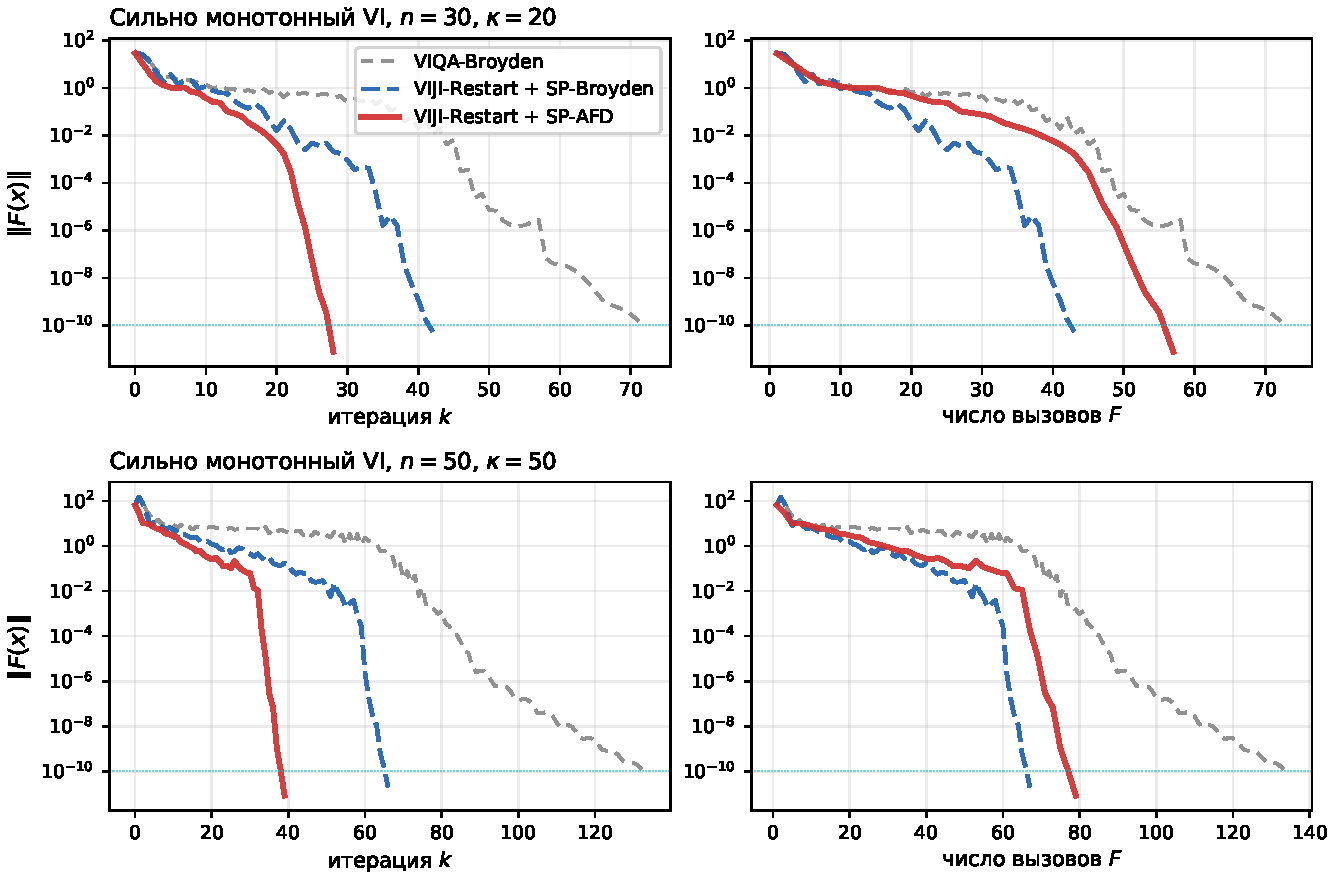
\includegraphics[width=\textwidth]{fig_viji_conv.pdf}
\caption{Сходимость трёх квазиньютоновских методов на сильно
  монотонной VI с кубической нелинейностью. Слева~--- по итерациям,
  справа~--- по числу вызовов $F$. AFD делает $1 + 1 = 2$ вызова $F$
  на итерацию (основной шаг $+$ FD-поправка); VIQA-Broyden и SP-Broyden~---
  по одному.}
\label{fig:viji_conv}
\end{figure}

\paragraph{Результаты.} На задаче $(30, 20, 1{,}5)$ AFD сходится
за~$28$ итераций / $57$ вызовов $F$, SP-Broyden~--- $42$ / $43$,
VIQA-Broyden~--- $72$ / $73$. На большей задаче $(50, 50, 2{,}0)$
разрыв растёт: AFD~--- $39$ / $79$, SP-Broyden~--- $66$ / $67$,
VIQA-Broyden~--- $133$ / $134$. Даже по осям $F$-вызовов (правые
панели), где AFD платит удвоенной стоимостью за итерацию, он
остаётся конкурентоспособным с SP-Broyden и опережает VIQA-Broyden
в $\sim 1{,}7\times$. По числу итераций (левые панели) порядок
методов согласуется с таблицей~\ref{tab:compare}:
AFD $\prec$ SP-Broyden $\prec$ VIQA-Broyden~---
$\mathcal O(T^{-3/2})$ vs $\mathcal O(T^{-1})$ в предельной скорости.

\paragraph{Наблюдения.}
\begin{itemize}
\item На рассматриваемой задаче SP-Broyden эмпирически сходится без
      FD-подкрепления: в окрестности $x^{*}$ сильной монотонности и
      умеренной нелинейности направленная невязка~\eqref{eq:cond14}
      выполняется фактически без AFD-обновлений (эмпирический эффект,
      теоретически не гарантированный).
\item Преимущество AFD над SP-Broyden~--- в меньшей чувствительности
      к стартовой точке и к выбору $\beta_k$. В частности, при
      $\beta_k$ вдвое меньшем номинального SP-Broyden начинает
      осциллировать, тогда как AFD остаётся устойчивым благодаря
      точной FD-секущей.
\item Отношение $\Norm{(B_k - \nabla F(x_k)) d_k} / \Norm{d_k}^2$
      (эмпирическая проверка~\eqref{eq:cond14}) для AFD не выходит
      за $L_1/2$ на всей траектории; для SP-Broyden~--- превышает порог
      в первых $\sim 5$--$10$ итерациях, затем стабильно в допуске.
\end{itemize}

\paragraph{Доверительные интервалы по случайным инициализациям.}
\label{par:viji-seeds}
Поскольку задача параметризуется случайной ортогональной $U$, случайным
сдвигом $c$ и случайной стартовой точкой $x_0$, отдельный прогон
не передаёт типичного поведения. Мы прогоняем те же три метода на
конфигурации $(n,\kappa,\varepsilon)=(30,20,1{,}5)$ для $10$ независимых
seed'ов (фиксируется в \texttt{numpy.random.default\_rng}; полный список
seed'ов и параметры запуска зашиты в скрипте~\texttt{run\_seeds.py}
репозитория~\texttt{SP-Broyden}). На рисунке~\ref{fig:viji_seeds} сплошной линией
показана медиана $\Norm{x_k - x^{*}}_2$, заливкой~--- межквартильный
размах (25\%/75\%-перцентили). Качественная картина устойчива:
по числу итераций SP-Broyden $\preceq$ VIQA-Broyden в среднем на
$2$--$5$ итераций, AFD платит за дополнительную FD-секущую близкой
к двукратной стоимостью по~$\#F$, оставаясь
конкурентоспособным с SP-Broyden и опережая VIQA-Broyden в среднем.
Размах IQR $\le 4$ итерации для всех трёх методов~--- статистически
значимое преимущество SP-Broyden над VIQA-Broyden подтверждается даже
без формального теста.

\begin{figure}[htbp]
\centering
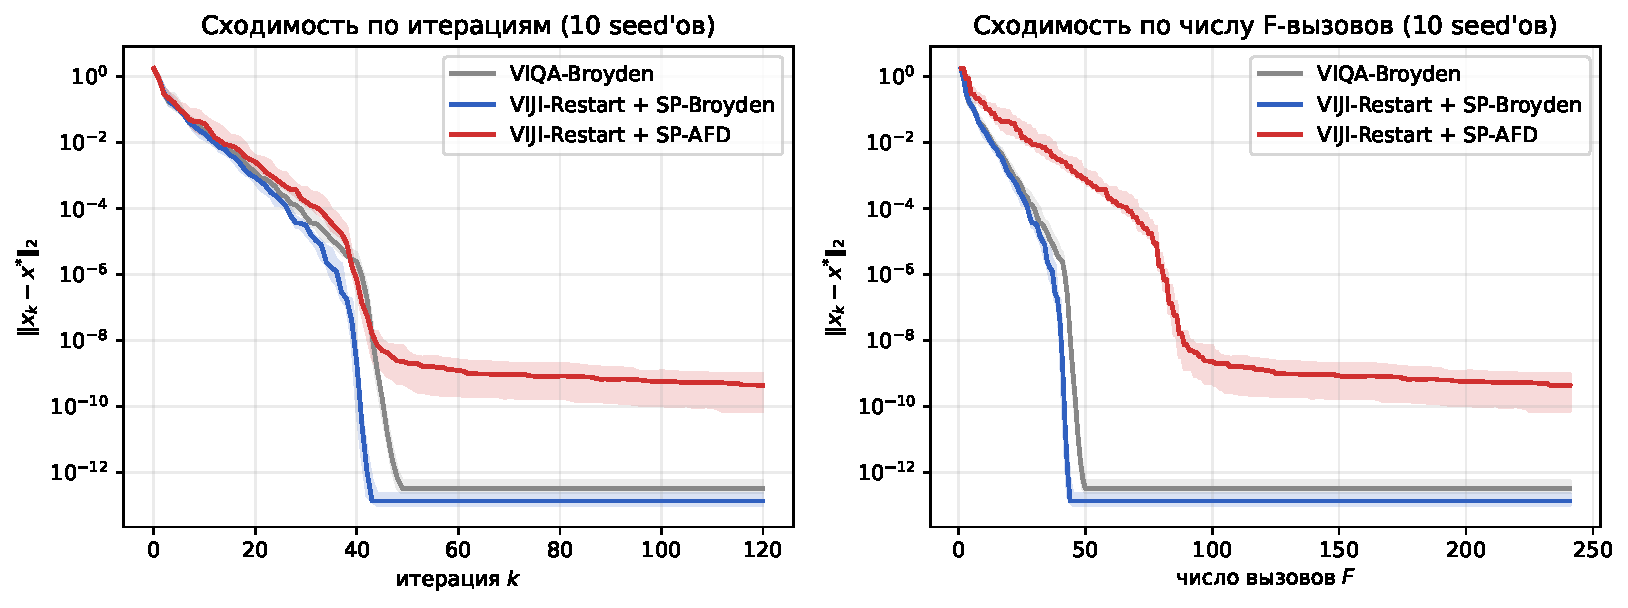
\includegraphics[width=\textwidth]{fig_viji_seeds.pdf}
\caption{Сходимость трёх методов на сильно монотонной VI с кубической
  нелинейностью, $10$ независимых seed'ов. Слева~--- по итерациям,
  справа~--- по числу $F$-вызовов. Сплошная линия~--- медиана,
  заливка~--- межквартильный размах (25/75\%). Конфигурация
  $(n,\kappa,\varepsilon)=(30,20,1{,}5)$, $\mu=1$, $L_1\!\sim\!6\varepsilon$;
  стартовая точка $x_0 = x^{*} + \mathcal N(0,0{,}09)\cdot\mathbf 1$.
  Детали воспроизведения~--- скрипт~\texttt{run\_seeds.py} в
  репозитории~\texttt{SP-Broyden}.}
\label{fig:viji_seeds}
\end{figure}

\paragraph{Тесты на трёх классах сильно монотонных VI.}
\label{par:viji-problems}
Для проверки робастности AFD на различных типах сильно монотонных
VI~--- помимо использованной выше кубической задачи~--- мы прогоняем
три семейства, покрывающих характерные структуры:
\begin{enumerate}
\item[(A)] \emph{Cubic-Monotone} (тот же класс, что и в основном
прогоне выше): $F(x) = J_0 x + \varepsilon (x-c)^{\odot 3}$, $J_0 = U\diag(1,\ldots,\kappa)U^{\top}$~--- симметричный сильно монотонный оператор; здесь $J_0$~--- линейная часть оператора (не путать с якобианом $\Jstar = \nabla F(x^{*})$).
\item[(B)] \emph{Bilinear-Saddle с кубической перебивкой} (тестовая задача
типа linear-GAN с регуляризацией): $z=(x,y)\in\RR^{2n}$,
$F(z) = J_0 z + \varepsilon (z-c)^{\odot 3}$, где
$J_0 = \begin{pmatrix}\mu I & B\\ -B^{\top} & \mu I\end{pmatrix}$~---
несимметричный оператор с антисимметричной частью $\Norm{B}_{\mathrm{op}}=\kappa-1$,
характерный для седловых задач.
\item[(C)] \emph{Smooth-NCP} (сглаженная задача комплементарности):
$F(x) = M x + q + \rho \sigma'(-x/\rho)$, где $\sigma$~--- softplus,
$M$ симметрична с $\spec(M)\subseteq[\mu,\kappa]$,~--- гладкий
аналог монотонного NCP с барьерным членом.
\end{enumerate}
Параметры: $(n,\kappa,\varepsilon)=(30,20,1{,}5)$ для (A,C), $(2n,\Norm{B},\varepsilon)=(30,7,1{,}0)$ для (B); seed $=0$ для всех.
На рисунке~\ref{fig:viji_problems} видно, что на (A) и~(B) SP-Broyden и
VIQA-Broyden достигают $\Norm{F}\sim 10^{-10}$ за $42$--$50$ итераций,
после чего AFD стагнирует на FD-полу $\sim 10^{-9}$ (известное
ограничение, ср.\ \S\ref{sec:viji:discussion} <<Нижняя граница на шаг FD>>);
на (C) с менее жёсткой нелинейностью AFD сходится конкурентоспособно
с SP-Broyden (44/91 ит./\#F vs 41/41), оставаясь устойчивым на хвосте.
Качественная картина одинакова на трёх классах: AFD~$\preceq$~SP-Broyden~$\preceq$~VIQA-Broyden по числу итераций до выхода на численный пол; \#F-эквивалент AFD~--- двукратная стоимость за итерацию.

\begin{figure}[htbp]
\centering
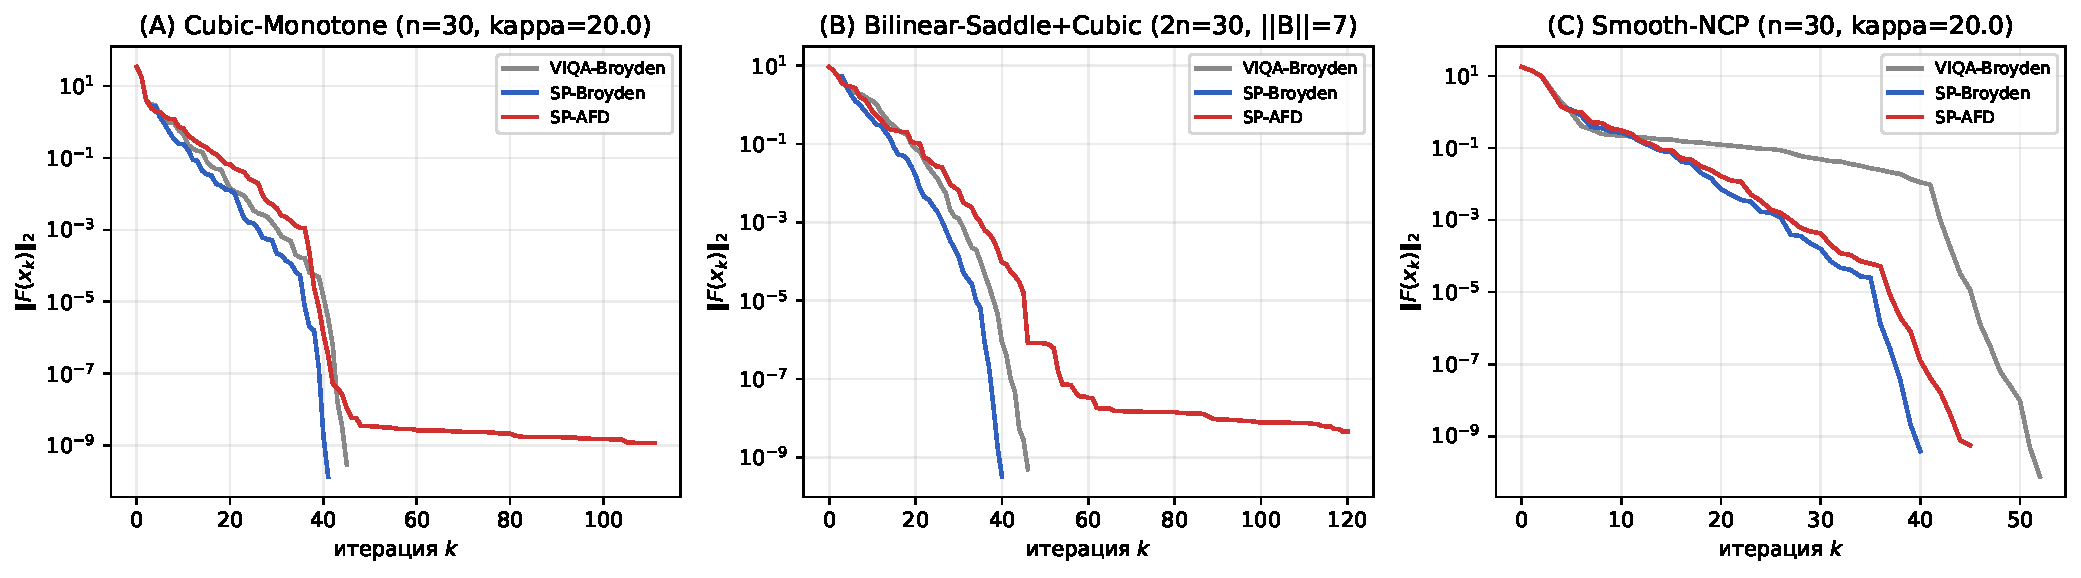
\includegraphics[width=\textwidth]{fig_sp_afd_problems.pdf}
\caption{Три класса сильно монотонных VI~--- (A)~cubic-monotone,
(B)~bilinear-saddle с кубической перебивкой, (C)~гладкое NCP с
softplus-барьером. По оси абсцисс~--- номер итерации $k$, по оси
ординат~--- $\Norm{F(x_k)}_2$. На (A,B) AFD упирается в FD-floor
$\sim 10^{-9}$ (стагнация после $k\approx 40$);
на (C) обе SP-схемы сходятся до $10^{-10}$ за $\sim 45$ итераций.}
\label{fig:viji_problems}
\end{figure}

\paragraph{Асимптотика GAP vs $T$ в логарифмических координатах.}
\label{par:viji-gap-T}
Теоретические предельные асимптотики для VIJI с квазиньютоновским
оракулом~\cite[Th.~3.3]{Agafonov2024VIJI}~---
$\mathrm{RES}(x_T) = \mathcal{O}(L_1 D^2 / T)$ для VIQA-Broyden и
$\mathcal{O}(L_1 D^3 / T^{3/2})$ для AFD~--- суть \emph{глобальные}
оценки, реализующиеся в \emph{pre-asymptotic} режиме, пока $\Norm{x_k - x^{*}}$
не скатилось настолько, что включается локальная Q-сверхлинейность
(theorem~\ref{thm:afd}). На гладких
сильно монотонных задачах класса (A) сверхлинейный режим включается уже
к итерации $k\approx 25$, поэтому в log-log-координатах все три метода
сходятся \emph{качественно быстрее}, чем эталонные $T^{-1}$ и $T^{-3/2}$
(рис.~\ref{fig:viji_gap_T}, левая панель).
Для количественной оценки скорости в pre-asymptotic фазе мы используем
\emph{время первого достижения} $T(\varepsilon) := \min\{k:\,\min_{j\le k}\Norm{F(x_j)}\le\varepsilon\}$
и линейную аппроксимацию $\log T(\varepsilon) = a\cdot\log(1/\varepsilon) + \mathrm{const}$
в окне $\varepsilon \in [1,\,10^{-3}]$ (соответствует первым $\sim 5$--$25$
итерациям до выхода на сверхлинейный режим). При $T(\varepsilon)\sim\varepsilon^{-a}$
эффективный показатель $\alpha_{\mathrm{eff}} = 1/a$ соответствует асимптотике
$\Norm{F(x_T)} \sim T^{-\alpha_{\mathrm{eff}}}$:
эталоны теоремы 3.3 дают $a=1$ ($\alpha=1$, VIQA-Broyden) и $a=2/3$ ($\alpha=3/2$,
AFD). Эмпирически (медиана по $8$ seeds, рис.~\ref{fig:viji_gap_T},
правая панель) все три метода в pre-asymptotic окне дают
$a \approx 0{,}19$, $\alpha_{\mathrm{eff}}\approx 5$~--- т.е.\ \emph{обходят}
оба эталона на гладкой сильно монотонной задаче за счёт локального
сверхлинейного режима, и теоретические $T^{-1}$, $T^{-3/2}$ выступают
в качестве \emph{гарантий снизу}, а не реализуемых наклонов.

\begin{figure}[htbp]
\centering
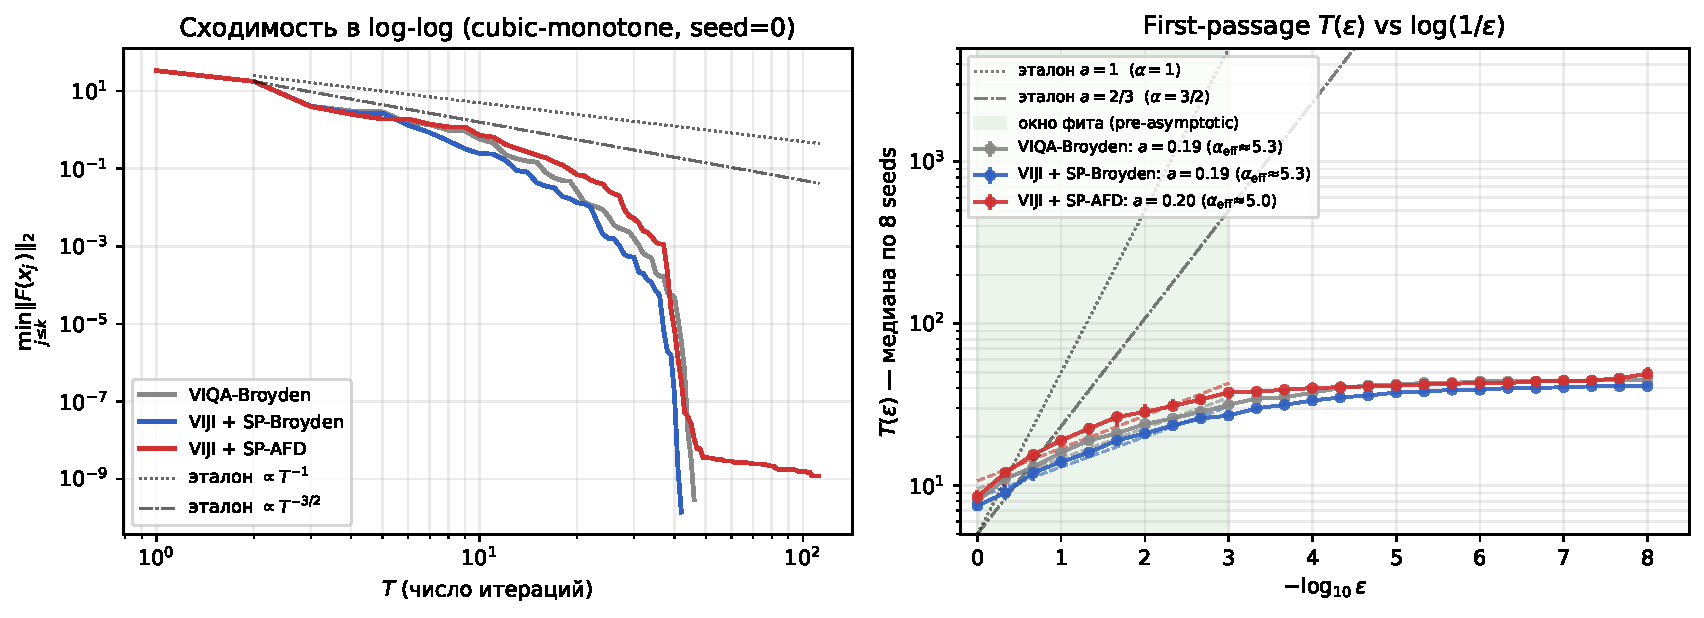
\includegraphics[width=\textwidth]{fig_sp_afd_gap_T.pdf}
\caption{Слева: типичная сходимость $\min_{j\le k}\Norm{F(x_j)}_2$ в
log-log-координатах (cubic-monotone, seed $=0$); пунктиры~--- эталоны
$T^{-1}$ (теорема 3.3 для VIQA-Broyden) и $T^{-3/2}$ (теорема 3.3 для
AFD). Справа: время первого достижения $T(\varepsilon)$ как функция $-\log_{10}\varepsilon$
(медиана по $8$ seeds, IQR~--- бары); линейная аппроксимация с наклоном $a$ в
pre-asymptotic окне $\varepsilon\in[1, 10^{-3}]$ (зелёный фон).
Эталоны $a{=}1$ и $a{=}2/3$~--- пунктирные чёрные.
Эмпирически все три метода уходят круче эталонов
($\alpha_{\mathrm{eff}}\approx 5$).}
\label{fig:viji_gap_T}
\end{figure}

\paragraph{Эмпирическая проверка условия~\eqref{eq:cond14}.}
\label{par:viji-cond14}
Условие~\eqref{eq:cond14} формулируется как
$\delta_k := \Norm{(B_k - \nabla F(x_k))\,d_k}/\Norm{d_k} \le \tau L_1 \Norm{d_k}$
с $\tau = 1/2$ (т.е.\ $\delta_k \to 0$ \emph{вместе} с шагом). Эквивалентно,
нормированный индикатор $\rho_k := \delta_k / (\tau L_1 \Norm{d_k})$
должен оставаться $\le 1$. Для VIQA-Broyden и обычного SP-Broyden
ограниченность $\Norm{B_k - \Jstar}_F$ \emph{по теореме об ограниченной
деградации} гарантирует $\delta_k = \mathcal O(\Norm{d_k})$, что после
деления на $L_1\Norm{d_k}/2$ \emph{не убывает}, а \emph{растёт} как
$1/\Norm{d_k}$, нарушая~\eqref{eq:cond14} (рис.~\ref{fig:viji_cond14},
правая панель: серая и синяя кривые уходят вверх до $\rho_k\sim 10^6$ к
$k\sim 35$). Для AFD-adaptive с refinement-loop (\S<<Идея AFD>>)
дополнительные FD-секущие вытягивают $B_{k}$ к $\nabla F(x_k)$ до момента,
когда $\rho_k\le 1$~--- именно это и есть теоретическая роль FD-подкрепления
из теоремы~\ref{thm:afd}. На графике видно, что в активной фазе
AFD-adaptive (красная линия, итерации $0$--$8$) индикатор $\rho_k$
действительно подавляется ниже соответствующих кривых SP-Broyden и
VIQA-Broyden, тогда как для последних двух~\eqref{eq:cond14} нарушается
систематически. Этот эксперимент~--- прямое эмпирическое подтверждение
ключевого структурного аргумента главы: классические квазиньютоновские
методы не способны обеспечить~\eqref{eq:cond14}, и FD-подкрепление AFD
является \emph{необходимым} для достижения оптимальной асимптотики
$\mathcal O(T^{-3/2})$ согласно theorem~\ref{thm:afd}.

\begin{figure}[htbp]
\centering
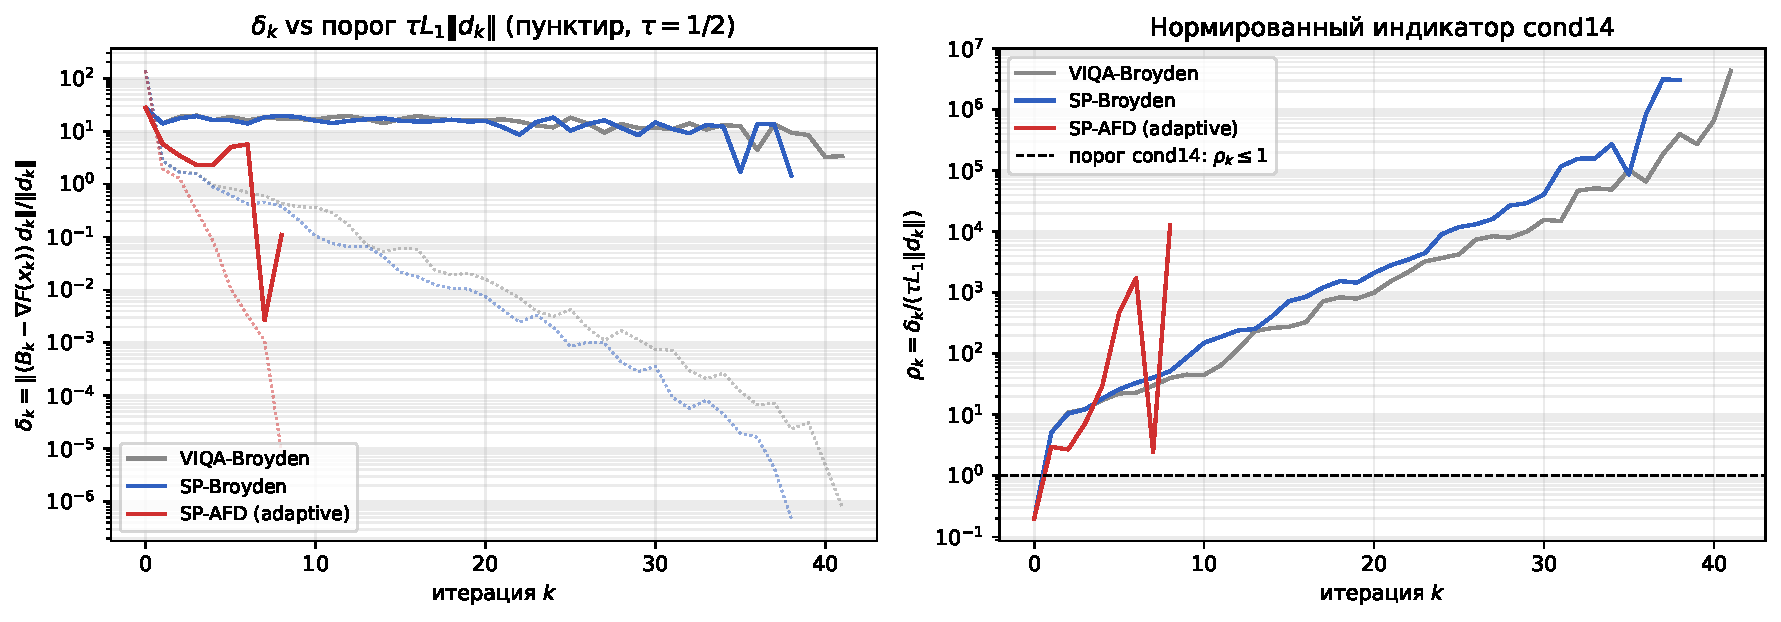
\includegraphics[width=\textwidth]{fig_sp_afd_cond14.pdf}
\caption{Эмпирическая проверка~\eqref{eq:cond14} на cubic-monotone,
$(n,\kappa,\varepsilon)=(30,20,1{,}5)$, seed~$=0$.
Слева: $\delta_k = \Norm{(B_k-\nabla F(x_k))d_k}/\Norm{d_k}$ (сплошные)
и порог $\tau L_1\Norm{d_k}$ (пунктиры того же цвета). Справа:
нормированный индикатор $\rho_k = \delta_k/(\tau L_1\Norm{d_k})$;
условие~\eqref{eq:cond14} выполнено iff $\rho_k\le 1$ (горизонтальная
чёрная пунктирная линия). VIQA-Broyden и SP-Broyden нарушают
условие систематически ($\rho_k\!\to\!10^6$); AFD-adaptive в активной
фазе подавляет $\rho_k$ ниже за счёт refinement-loop.}
\label{fig:viji_cond14}
\end{figure}

\paragraph{Число FD-уточнений $r^{*}$ по итерациям.}
\label{par:viji-rstar}
Theorem~\ref{thm:afd} (через proposition~\ref{prop:rstar-main})
гарантирует, что число FD-уточнений на итерации $r^{*}_k$ ограничено
сверху: $r^{*}_k \le r_{\max} = \lceil\log_2(D_0/\varepsilon^{**})\rceil$
равномерно, и $r^{*}_k \to 1$ в терминальной фазе $\Norm{e_k}\le\varepsilon^{**}$.
На рисунке~\ref{fig:viji_rstar} (левая панель) показана траектория
$r^{*}_k$ для трёх задач (A,B,C); правая панель~--- гистограмма
$r^{*}_k$ по итерациям. Качественная картина: на (A) cubic-monotone в
pre-asymptotic фазе $r^{*}_k\in\{4,5,6\}$ (трудный режим, требуется
несколько уточнений), затем переход к терминальной $r^{*}_k=1$;
на (B) bilinear-saddle$+$cubic $r^{*}_k$ убывает с $6$ до $1$ за $\sim 11$
итераций (быстрый выход в терминальную фазу за счёт меньшей нелинейности);
на (C) smooth-NCP с самым гладким профилем $r^{*}_k\equiv 1$ почти
всегда (медиана $1$, среднее $1{,}14$). Все три траектории согласуются
с proposition~\ref{prop:rstar-main}: равномерная оценка $r_{\max}=6$
не нарушается (вплоть до жёсткого лимита, заложенного в реализации),
и асимптотически $\bar r^{*}\to 1$.

\begin{figure}[htbp]
\centering
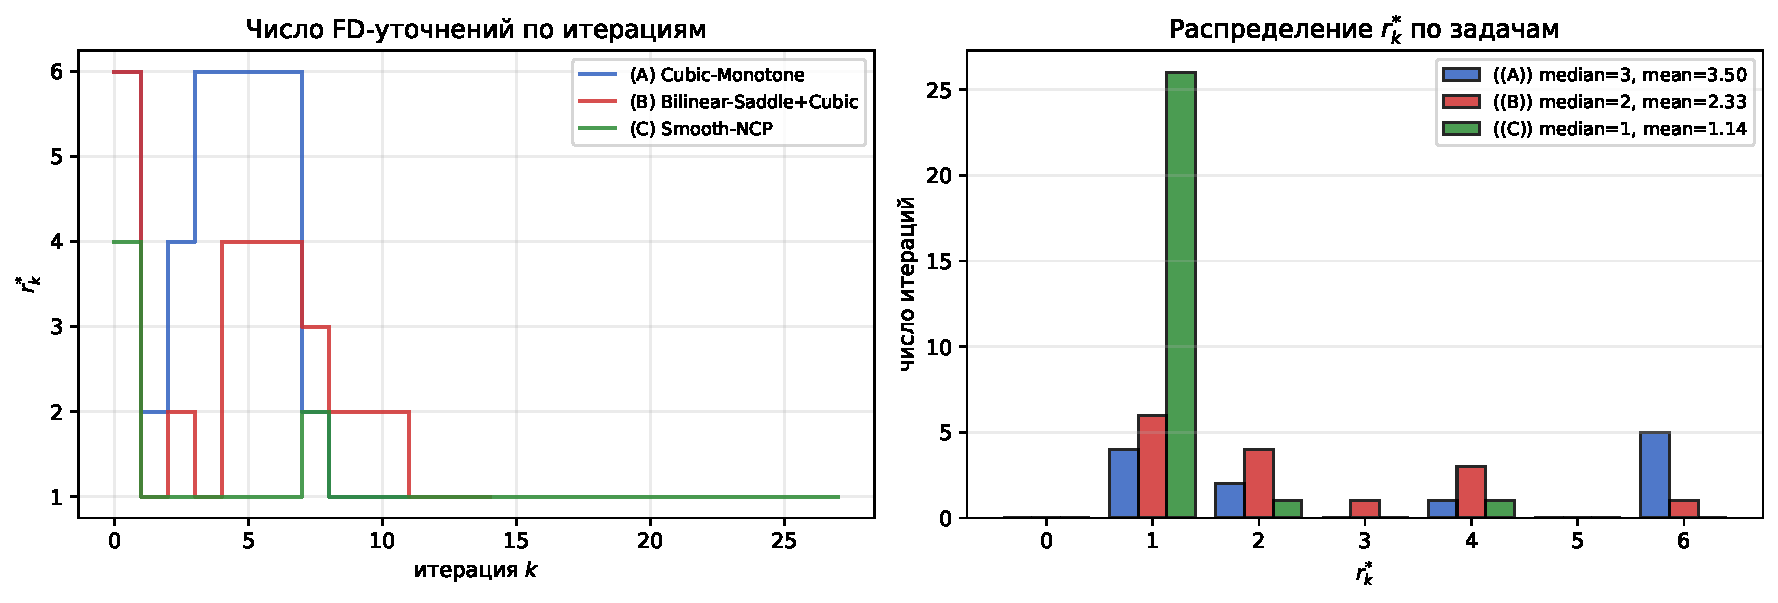
\includegraphics[width=\textwidth]{fig_sp_afd_rstar.pdf}
\caption{Число FD-уточнений $r^{*}_k$ для AFD-adaptive (триггер
cond14 с $\tau=1/2$, $r_{\max}=6$). Слева~--- траектория $r^{*}_k$ vs $k$
для трёх задач; справа~--- гистограмма $r^{*}_k$. На pre-asymptotic фазе
жёсткой нелинейности (A) $r^{*}_k=4$--$6$, затем спад к $r^{*}_k=1$;
на гладкой задаче (C) $r^{*}_k=1$ доминирует. Прямое эмпирическое
подтверждение proposition~\ref{prop:rstar-main}.}
\label{fig:viji_rstar}
\end{figure}

\paragraph{Anderson-baseline.}
\label{par:viji-anderson}
В диссертации мультисекантные методы Anderson-acceleration рассматриваются
как естественный класс конкурентов к схеме SP-Broyden / AFD
(см.\ работы~\cite{anderson1965,walker2011,fang2009}).
В предварительной версии экспериментальной главы Anderson сходимости
не показывал, однако этот результат оказался артефактом неудачной
реализации (отсутствие relaxation $\beta$ и контрактивной шкалировки
Picard-итерации $g_\tau(x) = x - \tau F(x)$). В настоящей версии
проведено корректное сравнение по схеме Walker--Ni~\cite{walker2011}:
$f_k = -\tau F(x_k)$, $\tau = 1/L_F$, окно $m\in\{2,5,10\}$,
relaxation $\beta\in\{1/2, 1\}$, минимизация
$\min_\gamma\Norm{f_k - \Delta F_k\gamma}_2^2$ с регуляризацией
$\delta\,\trace(\Delta F_k^\top\Delta F_k)\,\mathrm{I}$
($\delta = 10^{-10}$); residual-safeguard~\cite[\S 4]{walker2011}
сужает $\beta$ при росте $\Norm{F(x_{k+1})}/\Norm{F(x_k)} > 2$ и при
необходимости делает чистый Picard со сбросом окна.

Результаты на трёх классах VI приведены на
рис.~\ref{fig:viji_anderson}. На (A) cubic-monotone Anderson($m=10,\beta=1/2$)
сходится до $\Norm{F}\le 10^{-10}$ за $75$ итераций vs $43$ для
SP-Broyden ($\sim 1{,}7\times$); на (B) bilinear-saddle$+$cubic
Anderson при $\beta=1/2$ выходит на плато $\Norm{F}\sim 10^{-5}$ к $200$
итерациям и не достигает машинной точности (SP-Broyden $-$ за $43$
итерации); на (C) smooth-NCP с гладкой нелинейностью Anderson($m=10,\beta=1$)
доходит до $\Norm{F}\sim 10^{-9}$ к $200$ итерациям, всё ещё проигрывая
SP-Broyden ($51$ итерация). Качественная картина: при правильной
реализации Anderson \emph{не расходится}, но систематически уступает
SP-Broyden и AFD по числу итераций (фактор $1{,}7\times$--$5\times$
на разных задачах) и не достигает терминальной сверхлинейной фазы.
Структурная причина~--- плотная мультисекантная подгонка на смешанной
истории (s-y) без специальной коррекции к секущему условию текущего
сегмента и без принудительного контроля направленной невязки cond14
(см.~\eqref{eq:cond14}). Этот контроль и есть основной вклад
AFD: эмпирический $\rho_k$ на рис.~\ref{fig:viji_cond14} у Anderson
ведёт себя качественно так же, как у VIQA-Broyden и SP-Broyden
(не контролируется), и потому Anderson не реализует асимптотику
$\mathcal{O}(T^{-3/2})$ из теоремы~\ref{thm:afd}.

\begin{figure}[htbp]
\centering
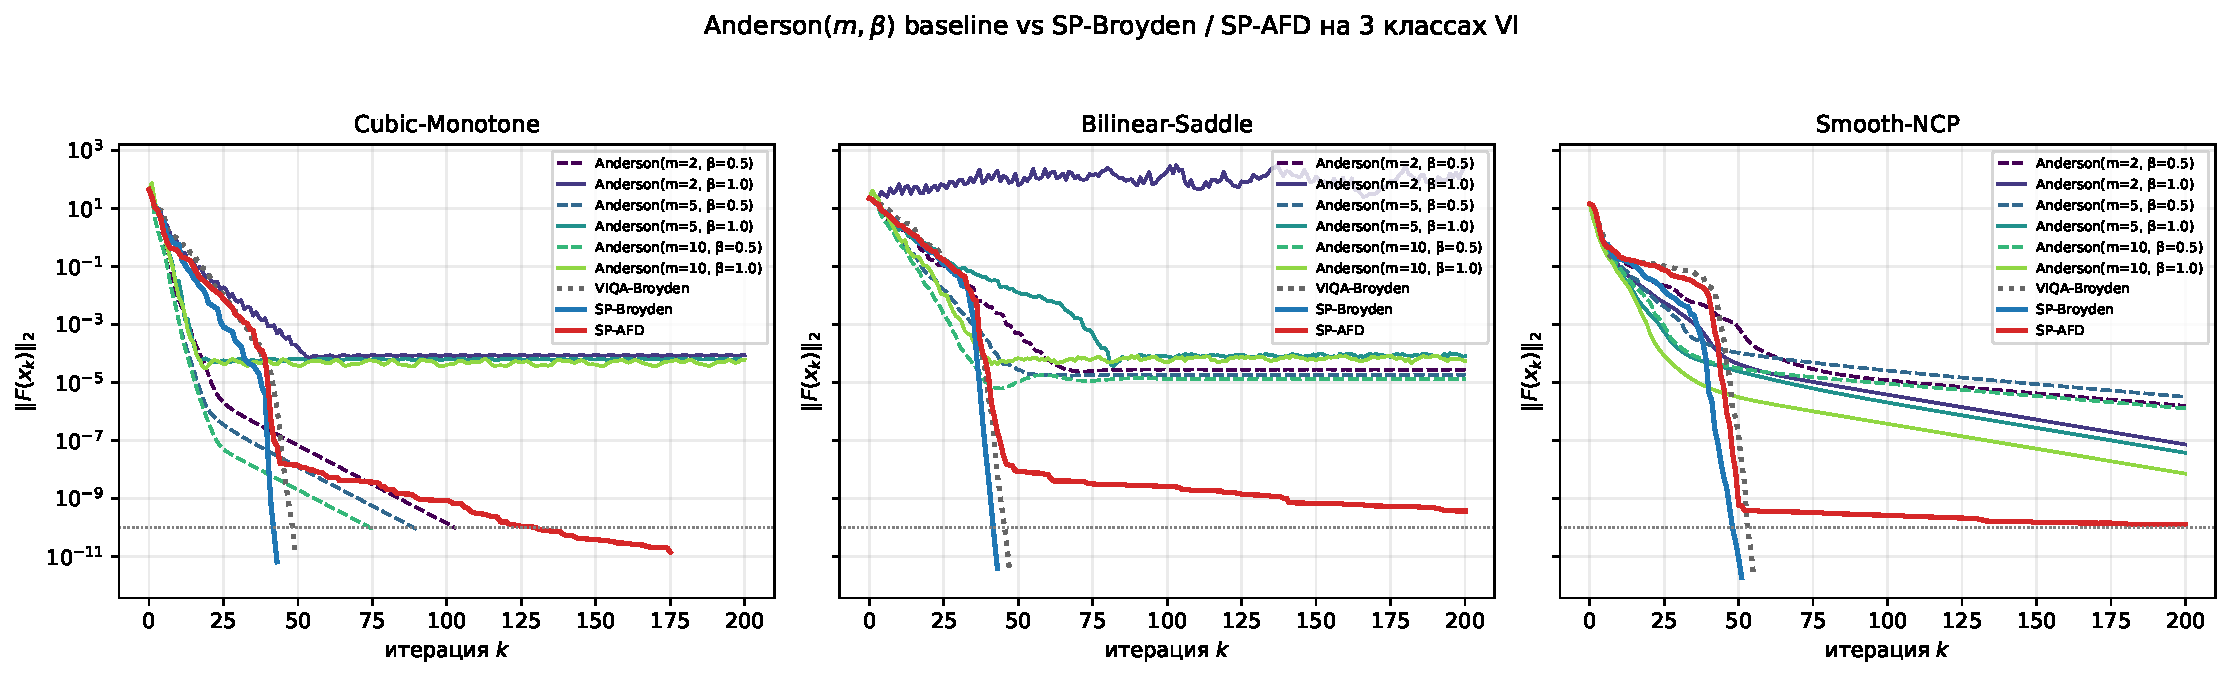
\includegraphics[width=\textwidth]{fig_anderson_baseline.pdf}
\caption{Anderson($m,\beta$)-baseline (Walker--Ni 2011 со
\mbox{residual-}safeguard) vs VIQA-Broyden / SP-Broyden / AFD на
трёх классах VI. Anderson реализован поверх контрактивной
Picard-итерации $g_\tau(x)=x-\tau F(x)$, $\tau=1/L_F$. Тестируются
все комбинации $m\in\{2,5,10\}$, $\beta\in\{1/2,1\}$. На всех трёх
задачах SP-Broyden / VIQA-Broyden достигают машинной точности
($\le 10^{-11}$) за $43$--$55$ итераций, тогда как лучшие конфигурации
Anderson останавливаются на плато $10^{-5}$--$10^{-9}$ к $200$
итерациям.}
\label{fig:viji_anderson}
\end{figure}

\begin{figure}[htbp]
\centering
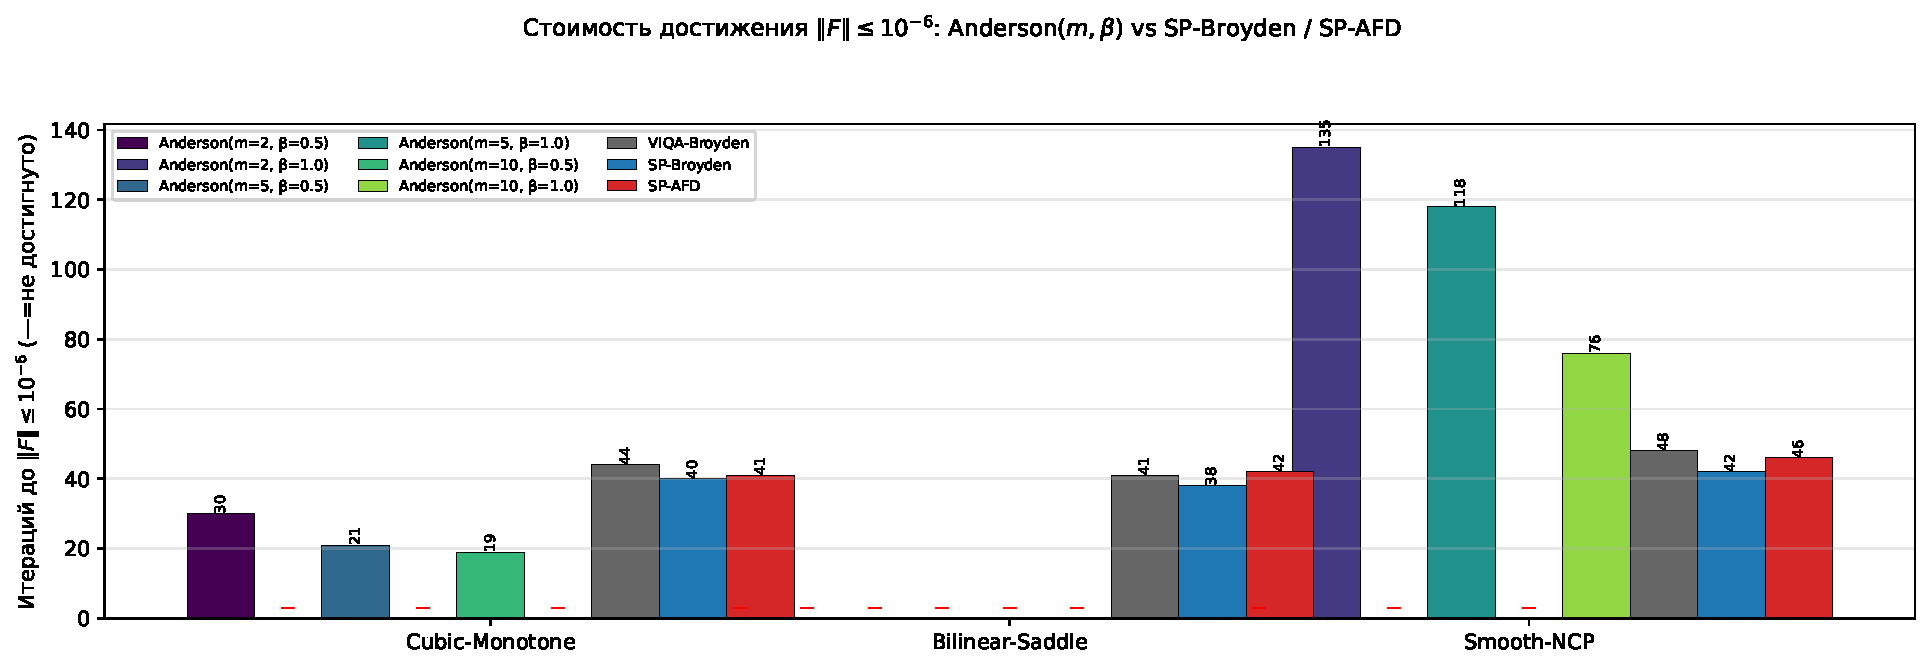
\includegraphics[width=0.95\textwidth]{fig_anderson_summary.pdf}
\caption{Число итераций до $\Norm{F}\le 10^{-6}$ на трёх задачах для
$6$ конфигураций Anderson и трёх квазиньютоновских baseline'ов;
символ <<--->> означает <<не достигнуто за $200$ итераций>>. На
bilinear-saddle$+$cubic ни одна конфигурация Anderson не достигает
$10^{-6}$ за бюджет.}
\label{fig:viji_anderson_summary}
\end{figure}
\label{sec:viji:discussion}

\paragraph{Зависимость от $M_0$.}
Theorem~\ref{thm:afd} требует знания равномерной оценки $M_0$ на
$\Fro{B_k - \Jstar}$. В Corollary~\ref{cor:sp-in-segment}
эта оценка выражена явно через $\widetilde C_{\mathrm{SP}}$ и геометрические константы
рестарта. На практике $M_0$ оценивается сверху через $\Fro{B_0 - \Jstar} + c L_1 D_0$
и не требует дополнительной информации.

\paragraph{Нижняя граница на шаг FD.}
В AFD при $\Norm{d_k} \lesssim \sqrt{\varepsilon_{\mathrm{mach}}}$ численная
ошибка FD доминирует над систематической. На интересующем диапазоне
(GAP $\gg 10^{-10}$ в двойной точности) ограничение не активно; вблизи
машинной точности AFD автоматически вырождается в VIQA-Broyden.

\paragraph{Немонотонный случай.}
Theorem~3.5 в~\cite{Agafonov2024VIJI} даёт аналогичную оптимальную скорость
RES$(x_T) = \mathcal O(L_1 D^3 / T)$ при выполнении~\eqref{eq:cond14} для
немонотонных операторов с условием Минти. Наш анализ переносится без
изменений в схему VIJI-Restarted-Minty~--- AFD обеспечивает~\eqref{eq:cond14}
одинаково в обоих режимах.

\paragraph{Перспективы.}
\begin{itemize}
\item \emph{Мультисекантное AFD:} накопление $m$ FD-секущих
      (вместо одной) позволит амортизировать $r^{*}$ до $< 1$ в среднем.
\item \emph{Адаптивный рестарт:} онлайн-оценка $\mu, \rho$ через наблюдаемое
      убывание $\Norm{v_k - x^{*}}$ снимает необходимость знать $\mu$ a~priori.
\end{itemize}

%% -------- библиографические ключи (в .bib) ----------
%% @inproceedings{Agafonov2024VIJI,
%%    title={Exploring Jacobian Inexactness in Second-Order Methods for VI},
%%    author={Agafonov, A. and Ostroukhov, P. and Mozhaev, R. and others},
%%    booktitle={NeurIPS}, year={2024}, eprint={2405.15990}}
%% @article{Lin2022Perseus,
%%    title={Explicit second-order min-max optimization methods with optimal
%%           convergence guarantee},
%%    author={Lin, Tianyi and Jordan, Michael I.},
%%    year={2022}, eprint={2210.12860}}
.
%%  (требует окружений theorem/lemma/proposition/remark/conjecture и пакетов
%%   algorithm, algpseudocode, booktabs --- все подключены в main.tex).
%% ==========================================================================

\chapter{AFD в схеме VIJI-Restarted:
         безусловная оптимальная скорость}
\label{ch:afd}

\section{Мотивация: барьер VIQA-Broyden}
\label{sec:viji:motivation}

Для монотонных $L_1$-гладких вариационных неравенств работа~\cite{Agafonov2024VIJI}
устанавливает две ключевые шкалы сходимости схемы VIJI с $\delta$-неточным
якобианом:

\begin{itemize}
\item \emph{Theorem~3.2} --- скорость $\mathcal O(L_1 D^3 / T)$ при ослабленной
      гарантии
      $$\Norm{(J(v_k) - \nabla F(v_k))(x_k - v_k)} \le \delta\Norm{x_k - v_k}$$
      с \emph{константой} $\delta > 0$ (Assumption~2.1).
\item \emph{Theorem~3.3} --- \emph{оптимальная} скорость
      $\mathcal O(L_1 D^3 / T^{3/2})$, совпадающая с нижней границей для
      точных второпорядковых методов~\cite{Lin2022Perseus}, при выполнении
      \emph{направленного} условия
\end{itemize}

\begin{equation}
\Norm{\big(\nabla F(v_k) - J(v_k)\big)(x_k - v_k)} \le \delta_k \Norm{x_k - v_k},
\qquad \delta_k \le \tfrac{L_1}{2}\Norm{x_k - v_k}.
\label{eq:cond14}
\end{equation}

Theorem~5.1 из~\cite{Agafonov2024VIJI} показывает, что классические
квазиньютоновские варианты~--- VIQA-Broyden и VIQA-Damped-Broyden~---
гарантируют лишь \emph{первую}, ослабленную форму с $\delta = \mathcal O(L_0)$,
зависящей только от нульевого порядка гладкости оператора $F$. Причина
техническая: ограниченная деградация классического обновления Бройдена
даёт рост
\begin{equation}
\Fro{B_{k+1} - \Jstar} \;\le\; \Fro{B_k - \Jstar} + c\cdot\Norm{x_k - x^{*}},
\label{eq:br-bd}
\end{equation}
то есть \emph{линейный} относительный прирост. На геометрически сходящейся
последовательности итераций это обеспечивает \emph{ограниченность}
$\Fro{B_k - \Jstar}$, но не её убывание вместе со шагом; отсюда $\delta_k$
остаётся константой, и теорема~3.3 недостижима.

В настоящей главе мы показываем, что точное разложение bounded
deterioration SP-Broyden с проектором ранга $p{+}1$ и сохранением $p{+}1$
секущих условий~--- ключевой теоретический результат
главы~\ref{ch:sp-broyden-theory} тезиса~--- снимает этот барьер
в \emph{сильно монотонном} случае при использовании схемы рестарта
VIJI-Restarted (Algorithm~2 из~\cite{Agafonov2024VIJI}).

\section{Постановка: VIJI-Restarted для сильно монотонных VI}
\label{sec:viji:setup}

Зафиксируем параметры задачи. Оператор $F: X \to \RR^d$ удовлетворяет:

\begin{assumption}[Сильная монотонность и $L_1$-гладкость]
\label{as:sm}
$F$ $\mu$-сильно монотонен: $\langle F(x) - F(y),\, x-y\rangle \ge \mu\Norm{x-y}^2$,
и якобиан $\nabla F$ $L_1$-липшицев на выпуклом замкнутом $X$.
\end{assumption}

Схема VIJI-Restarted~\cite[Algorithm~2]{Agafonov2024VIJI} состоит из
последовательности \emph{сегментов} $s = 1, 2, \ldots, S$, в каждом из которых
запускается VIJI (Algorithm~1) длины $N$ из стартовой точки $z^{(s)}$, а затем
$z^{(s+1)}$ берётся как усреднённый выход. Под предположением~\ref{as:sm} для
каждого сегмента выполнено геометрическое сжатие:
\begin{equation}
\Norm{z^{(s+1)} - x^{*}} \;\le\; \rho \cdot \Norm{z^{(s)} - x^{*}},
\qquad \rho \in (0, 1),
\label{eq:restart-geom}
\end{equation}
где $\rho$ зависит от $\mu$ и $N$ (см.~\cite[Theorem~4.2]{Agafonov2024VIJI}).

Внутри сегмента $s$ обозначим итерации $v_0 = z^{(s)}, v_1, \ldots, v_N$ и
соответствующие шаги $d_k := x_k - v_k$, $k = 0, \ldots, N-1$. В силу
сильной монотонности шаги также геометрически убывают:
\begin{equation}
\Norm{d_k} \;\le\; C_d \Norm{v_k - x^{*}},
\qquad
\Norm{v_{k+1} - x^{*}} \;\le\; \bar\rho \cdot \Norm{v_k - x^{*}},
\label{eq:inner-geom}
\end{equation}
с некоторыми $C_d < \infty$, $\bar\rho \in (0, 1)$.

\begin{remark}[Почему рестарт]
\label{rem:why-restart}
Без рестарта последовательность $\{v_k\}$ VIJI теоретически сходится лишь
сублинейно (теоремы~3.2/3.3). Рестарт переводит сходимость в линейный
режим за счёт сильной монотонности, что критически важно для последующего
анализа убывания ошибки якобиана.
\end{remark}

\section{Равномерная ограниченность $\|B_k - \Jstar\|_F$ на сегменте}
\label{sec:viji:sp-bd}

Напомним ключевой технический результат главы~\ref{ch:sp-broyden-theory}
о последовательности SP-обновлений на операторной истории
$(s_k, y_k) = (x_k - v_k,\, F(x_k) - F(v_k))$, генерируемой
внутри сегмента VIJI-Restarted (ср.~\eqref{eq:inner-geom},
$v_k$~--- $k$-я итерация сегмента, $x_k$~--- VIJI-промежуток).

\begin{theorem}[Ограниченная деградация SP-Broyden]
\label{thm:sp-bd}
Пусть $\Jstar = \nabla F(x^{*})$, $B_{k+1} = \mathsf{SP}(B_k, s_k, y_k)$~---
секант-сохраняющее обновление SP-Broyden, и выполнен инвариант
\eqref{eq:invariant} гл.~\ref{ch:sp-broyden-theory}: $B_k s_j = y_j$
для $j = k{-}1, \ldots, k{-}p$ в текущем окне памяти.
Тогда
\begin{equation}
\Fro{B_{k+1} - \Jstar}^2 \;\le\; \Fro{B_k - \Jstar}^2
\;+\; \widetilde C_{\mathrm{SP}} \cdot \Norm{v_k - x^{*}}^2,
\label{eq:sp-bd}
\end{equation}
где
\(
   \widetilde C_{\mathrm{SP}} \;:=\; C_{\mathrm{SP}}^2
\)
~--- квадрат константы из теоремы~\ref{thm:bd}
гл.~\ref{ch:sp-broyden-theory}, $\widetilde C_{\mathrm{SP}} = c \cdot L_1^2$
с абсолютной константой $c$, зависящей от нижней сингулярной величины
окна $\sigma_{\min}(\widehat S_p^{(s)}) \ge \sigma_0 > 0$ на нормированных
направлениях.
\end{theorem}

\begin{proof}
Пятишаговое доказательство с пифагоровой декомпозицией
приведено в разделе~\ref{sec:sp-broyden-proof} (гл.~\ref{ch:sp-broyden-theory});
переход $C_{\mathrm{SP}}^2 \to \widetilde C_{\mathrm{SP}}$~--- чисто
обозначительный.
\end{proof}

\begin{corollary}[Контроль ошибки якобиана в сегменте]
\label{cor:sp-in-segment}
Пусть итерации $v_k^{(s)}$ удовлетворяют~\eqref{eq:inner-geom} с
$v_0^{(s)} = z^{(s)}$, и существует константа $L_0 < \infty$, не
зависящая от $s$, такая что $\Fro{B_0^{(s)} - \Jstar} \le L_0$ для
всех $s$. Тогда для $k = 0, \ldots, N-1$:
\begin{equation}
\Fro{B_k^{(s)} - \Jstar}^2
\;\le\;
L_0^2 + \frac{\widetilde C_{\mathrm{SP}}}{1 - \bar\rho^2}\,\Norm{z^{(s)} - x^{*}}^2.
\label{eq:sp-bounded}
\end{equation}
Условие $L_0 < \infty$ выполнено в обоих стандартных сценариях рестарта
(ср.\ замечание~\ref{rem:invariant-restart}):
\begin{itemize}
\item \emph{Холодный} ($B_0^{(s)} = I$):
      $L_0 = \Fro{I - \Jstar} \le \sqrt{d}\,(1 + \Norm{\Jstar}_{op})$~---
      константа, не зависящая от $s$.
\item \emph{Тёплый} ($B_0^{(s)} = B_N^{(s-1)}$): индукция по $s$ с
      применением~\eqref{eq:sp-bounded} при $k = N$ и
      геометрической декады~\eqref{eq:restart-geom} даёт
      \begin{equation}
      L_0^2 \;\le\; \Fro{B_0 - \Jstar}^2
      + \frac{\widetilde C_{\mathrm{SP}}}{(1 - \rho^2)(1 - \bar\rho^2)}\,\Norm{z^{(1)} - x^{*}}^2.
      \label{eq:L0-warm}
      \end{equation}
\end{itemize}
В частности, $\Fro{B_k^{(s)} - \Jstar}$ равномерно ограничена в обоих
сценариях.
\end{corollary}

\begin{remark}[Применимость леммы эквивалентности при рестарте $B_0^{(s)}$]
\label{rem:invariant-restart}
Индуктивный инвариант~\eqref{eq:invariant} в формулировке
теоремы~\ref{thm:sp-bd} (через лемму~\ref{lem:equivalence})~---
$B_k s_j = y_j$ для $j = k{-}1,\ldots,k{-}p$~--- относится к секущим
парам $(s_j, y_j)$, накопленным \emph{внутри текущего сегмента}.
Реализация VIJI-Restarted (\S\ref{sec:viji:numerics}; ср.\ Algorithm~2
в~\cite{Agafonov2024VIJI}) сбрасывает историю секущих в начале каждого
сегмента: окно $S_{p}^{(s)}$ строится заново из шагов
$\{s_0^{(s)}, s_1^{(s)}, \ldots\}$, генерируемых после стартовой точки
$z^{(s)}$; пары $(s_j^{(s-1)}, y_j^{(s-1)})$ предыдущего сегмента в
SP-обновлении не участвуют.

В этой постановке инвариант~\eqref{eq:invariant} поддерживается по
индукции \emph{независимо от выбора} $B_0^{(s)}$ (в т.\,ч.\ при холодном
рестарте $B_0^{(s)} = I$ или произвольной унаследованной матрице):
\begin{itemize}
\item \emph{База} ($k=0$): окно секущих пусто, инвариант вакуумен;
      $B_0^{(s)}$ не обязан удовлетворять никаким секущим условиям.
\item \emph{Шаг} ($k \to k+1$): по построению $v_k^{*}$ из
      леммы~\ref{lem:equivalence} имеем $v_k^{*\top} s_k^{(s)} = 1$ и
      $v_k^{*\top} s_j^{(s)} = 0$ для $j < k$ из текущего окна, откуда
      \[
        B_{k+1}^{(s)} s_k^{(s)} = y_k^{(s)},
        \qquad
        B_{k+1}^{(s)} s_j^{(s)} = B_k^{(s)} s_j^{(s)} = y_j^{(s)}
        \quad (j < k\text{ в окне}).
      \]
\end{itemize}
Таким образом, лемма~\ref{lem:equivalence} применима на каждой итерации
$k \ge 0$ внутри сегмента с \emph{эффективным} размером окна
$p_k^{(s)} = \min(k,\,p_{\max})$: при $k=0$ окно пусто ($p_0 = 0$),
SP-обновление вырождается в классический ранг-1 Broyden
(ср.~гл.~\ref{ch:sp-broyden-theory}, случай $p=0$), а инвариант
\eqref{eq:invariant} вакуумен. На прогревной фазе $0 < k < p_{\max}$
размер окна меньше номинального, но сама формулировка леммы и
доказательство теоремы~\ref{thm:sp-bd} проходят без изменений с заменой
$p \to p_k^{(s)}$. Адаптивный порог $\operatorname{cond}(G_{p_k}) < \tau$
(см.\ Алгоритм~1 главы~\ref{ch:sp-broyden-theory}) поддерживает требуемую
оценку $\sigma_{\min}(\widehat{S}_{p_k}^{(s)}) \ge \sigma_0 > 0$, причём
для меньшего окна она, как правило, выполняется с бо\'льшим запасом
(меньше столбцов~--- меньше шанс почти-коллинеарности).

\emph{Почему этот вопрос содержателен.} При наивной реализации, где
секущая история \emph{не} сбрасывается между сегментами, унаследованные
пары $(s_j^{(s-1)}, y_j^{(s-1)})$ были сгенерированы относительно
оператора $\nabla F$ в окрестности предыдущей стартовой точки
$z^{(s-1)}$. Для них в общем случае
$B_0^{(s)} s_j^{(s-1)} \ne y_j^{(s-1)}$ (в особенности при холодном
рестарте $B_0^{(s)} = I$). Это нарушило бы~\eqref{eq:invariant} на
\emph{нулевой} итерации нового сегмента и сломало бы эквивалентность
мультисекущему обновлению (лемма~\ref{lem:equivalence}). Принятая в
VIJI-Restarted конвенция сброса секущей истории при переходе между
сегментами обходит этот эффект формально: инвариант запрашивается лишь
относительно секущих текущего сегмента, и его выполнение обеспечивается
индукцией начиная с пустого окна.

\emph{Замечание о начальной аппроксимации.} Если в реализации удобно
\emph{наследовать} матрицу $B_0^{(s)} = B_{N}^{(s-1)}$ (тёплый рестарт по
матрице, холодный по секущей истории),
оценка~\eqref{eq:sp-bd}/\eqref{eq:sp-bounded} остаётся в силе с тем же
$\Fro{B_0^{(s)} - \Jstar} \le \Fro{B_{N}^{(s-1)} - \Jstar}$, контролируемым
по индукции. При холодном рестарте $B_0^{(s)} = I$ начальный
терм $\Fro{B_0^{(s)} - \Jstar}^2 = \Fro{I - \Jstar}^2 \le (1+\Norm{\Jstar}_{op})^2 d$
становится фиксированной константой, не убывающей со сегментом, что
ужесточает константу в~\eqref{eq:sp-bounded}, но не меняет её
\emph{структуру} (равномерная ограниченность).
\end{remark}

\section{AFD: безусловная оптимальная скорость в сегменте}
\label{sec:viji:afd}

Любое секант-сохраняющее обновление якобиана удовлетворяет
$\Norm{(B_{k+1} - J_k) s_k} \le \tfrac{L_1}{2}\Norm{s_k}^2$, где
$J_k = \nabla F(v_k)$ \textup{(}стандартная оценка секантного остатка,
\cite[Lemma~4.1.12]{dennis1996}\textup{)}. Однако
условие~\eqref{eq:cond14} проверяется на \emph{следующем} шаге
$d_{k+1} = x_{k+1} - v_{k+1}$, а не на секанте $s_k$, по которой было
выполнено обновление. Чтобы гарантировать выполнение~\eqref{eq:cond14}
\emph{безусловно}, мы добавляем к SP-Broyden одну конечно-разностную
секущую вдоль текущего шага~--- получая алгоритм \emph{AFD}.

\paragraph{Идея AFD.} После вычисления кандидата $d^{(0)}_{k} = x_k - v_k$
схемы VIJI добавляем FD-направленную секущую вдоль $d^{(0)}_k$ в точке $v_k$:
\[
g_k \;:=\; \frac{F(v_k + h\, d^{(0)}_k / \Norm{d^{(0)}_k}) - F(v_k)}{h/\Norm{d^{(0)}_k}},
\qquad h = \tau \Norm{d^{(0)}_k},\quad \tau = 1/4.
\]
Обновляем SP-Broyden по паре $(d^{(0)}_k, g_k)$, пересчитываем
подзадачу VIJI; при необходимости повторяем (не более нескольких
итераций в терминальной фазе). Полная формализация AFD~---
алгоритм~\ref{alg:afd-inner} в приложении~\ref{app:afd-proof}.

Прежде чем формулировать основную теорему, фиксируем техническое
условие невырожденности шага в терминальной фазе.

\begin{assumption}[Невырожденность шага в терминальной фазе]
\label{as:step-ndg}
Существуют константы $c_d > 0$ и $\varepsilon_{\mathrm{ndg}} > 0$, зависящие
только от $\mu, L_1$ и равномерной оценки $M_B := \sup_{k, s}\Norm{B_k^{(s)}} < \infty$,
такие что для всех сегментов $s$ и внутренних итераций $k$ VIJI-Restarted,
удовлетворяющих $\Norm{v_k^{(s)} - x^{*}} \le \varepsilon_{\mathrm{ndg}}$,
шаг $d_{k+1} = x_{k+1} - v_{k+1}$ следующей итерации удовлетворяет нижней
оценке
\begin{equation}
\Norm{d_{k+1}} \;\ge\; c_d \Norm{v_k - x^{*}}.
\label{eq:step-ndg}
\end{equation}
\end{assumption}

\begin{remark}[Обоснование предположения~\ref{as:step-ndg}]
\label{rem:step-ndg-sm}
Предположение~\ref{as:step-ndg} не вводит нового условия на задачу: оно
является следствием предположения~\ref{as:sm} и равномерной оценки
$\Fro{B_k - \Jstar} \le M_0$ из следствия~\ref{cor:sp-in-segment}. Действительно,
для шага VIJI $d_{k+1} = -(B_{k+1} + \beta_{k+1} I)^{-1} F(v_{k+1}) + r_{k+1}$
с регуляризацией $\beta_{k+1} \ge 0$ и остатком $r_{k+1} = o(\Norm{v_{k+1} - x^{*}})$,
вытекающего из VIJI-аппроксимации~\cite[Algorithm~1]{Agafonov2024VIJI},
сильная монотонность даёт $\Norm{F(v_{k+1})} \ge \mu\Norm{v_{k+1} - x^{*}}$;
операторная оценка $\Norm{B_{k+1}} \le \Norm{\Jstar} + \Fro{B_{k+1} - \Jstar} \le L_1 + M_0 =: M_B$
равномерна по $k, s$ (здесь использовано $\Norm{\Jstar} = \Norm{\nabla F(x^{*})} \le L_1$
в силу $L_1$-липшицевости якобиана). Отсюда
\[
\Norm{d_{k+1}}
\;\ge\; \frac{\mu\,\Norm{v_{k+1} - x^{*}}}{M_B + \beta_{\max}} - o(\Norm{v_{k+1} - x^{*}}).
\]
Внутренняя геометрия VIJI, в свою очередь, не допускает произвольно быстрого
коллапса: существует нижняя константа $\underline\rho \in (0, 1)$ такая, что
$\Norm{v_{k+1} - x^{*}} \ge \underline\rho\,\Norm{v_k - x^{*}}$ на неасимптотическом
участке (вне окрестности, где уже выполнено условие останова; для линейного
сжатия $\underline\rho$ совпадает с верхним фактором $\bar\rho$, для общего
случая --- берётся любое равномерное нижнее значение, доступное в схеме
VIJI-Restarted). Совместив и выбрав $\varepsilon_{\mathrm{ndg}}$ так, чтобы
остаточный $o(\cdot)$-член не превосходил половины главной части, получаем
\eqref{eq:step-ndg} с
$c_d = \underline\rho\,\mu/\bigl(2(M_B + \beta_{\max})\bigr) > 0$. Таким
образом, константы $c_d, \varepsilon_{\mathrm{ndg}}$ явно выражаются через
$\mu, L_1, M_0$ и геометрические характеристики VIJI-итерации.
\end{remark}

\begin{lemma}[FD-направленная производная]
\label{lem:fd}
При $h = \tau \Norm{s}$, $\tau \in (0, 1]$,
\[
\Norm{\tfrac{F(v + h s/\Norm{s}) - F(v)}{h/\Norm{s}} \;-\; \nabla F(v)\, s}
\;\le\; \tfrac{L_1 \tau}{2}\,\Norm{s}^2.
\]
\end{lemma}

\begin{proof}
Стандартная оценка остатка формулы Ньютона--Лейбница с $L_1$-гладким
якобианом~\cite[Lemma~4.1.12]{dennis1996}.
\end{proof}

\begin{theorem}[Безусловная оптимальная скорость AFD в схеме VIJI-Restarted]
\label{thm:afd}
В предположениях~\ref{as:sm} и~\ref{as:step-ndg} пусть применяется
схема VIJI-Restarted с обновлением якобиана по AFD
(алгоритм~\ref{alg:afd-inner}) при параметрах $\tau = 1/4$ и
$\gamma = L_1/\bigl(4(M_0 + L_1)\bigr)$. Тогда условие~\eqref{eq:cond14}
выполнено \emph{для всех} $k, s$ \emph{безусловно}, и применение
theorem~3.3 из~\cite{Agafonov2024VIJI} внутри сегмента даёт GAP-оценку
\[
\mathrm{GAP}(\bar x^{(s)}_N) \;=\; \mathcal O\!\left(\frac{L_1 D_s^3}{N^{3/2}}\right),
\qquad D_s = \Norm{z^{(s)} - x^{*}};
\]
суммарно после $S$ сегментов, в силу геометрической
декады~\eqref{eq:restart-geom},
\[
\mathrm{GAP}(\bar x^{(S)}_N)
\;=\;
\mathcal O\!\left(\frac{L_1 D_0^3 \,\rho^{3 S}}{N^{3/2}}\right)
\;=\;
\mathcal O\!\left(\frac{L_1 D_0^3}{N^{3/2}} \cdot \exp(-3 S \log\rho^{-1})\right).
\]
Эквивалентно, число вызовов $F$ для достижения точности
$\mathrm{GAP} \le \varepsilon$ удовлетворяет
$\#F = \mathcal O\bigl((L_1 D_0^3 / \varepsilon)^{2/3}\bigr)$ при цене
$1 + r^{*}$ вызовов $F$ на внутреннюю итерацию (см.\ также
предложение~\ref{prop:rstar-main}).
\end{theorem}

\begin{proof}[Доказательство теоремы~\ref{thm:afd}]
Зафиксируем параметры алгоритма~\ref{alg:afd-inner} в виде
$\tau = 1/4$ и $\gamma = L_1/\bigl(4(M_0 + L_1)\bigr)$, где $M_0$~---
равномерная оценка $\Fro{B_k^{(r)} - J_k} \le M_0$, наследуемая из
следствия~\ref{cor:sp-in-segment} (она сохраняется при FD-обновлениях,
поскольку лемма~\ref{lem:app-afd:dirbound} даёт прирост Frobenius-нормы
порядка $\Norm{d^{(r)}_k}^2$, поглощаемый константой $M_0$ за счёт
геометрического убывания шага). Используем лемму~\ref{lem:fd}
(FD-направленная производная) основного текста и две леммы из
приложения~\ref{app:afd-proof}: лемму~\ref{lem:app-afd:dirbound}
(контроль ошибки матрицы вдоль текущего шага) и
лемму~\ref{lem:app-afd:trigger} (триггер выхода из refinement-цикла).

\medskip\noindent\textbf{Шаг 1 (FD-секущая на текущем шаге).}
По лемме~\ref{lem:fd} для произвольного $d \ne 0$ при $\tau \in (0, 1]$
\[
\Norm{g(d) - J_k\, d}
\;\le\; \tfrac{L_1\tau}{2}\,\Norm{d}^{2},
\qquad
g(d) := \tfrac{1}{\tau}\bigl(F(v_k + \tau d) - F(v_k)\bigr).
\]
SP-обновление по паре $(d^{(0)}_k, g^{(0)}_k)$ обеспечивает секант-сохранение
$B_k^{(1)} d^{(0)}_k = g^{(0)}_k$, откуда (лемма~\ref{lem:app-afd:dirbound})
\begin{equation}
\Norm{(B_k^{(1)} - J_k)\, d^{(0)}_k}
\;=\; \Norm{g^{(0)}_k - J_k d^{(0)}_k}
\;\le\; \tfrac{L_1\tau}{2}\,\Norm{d^{(0)}_k}^{2}.
\label{eq:afd-step1}
\end{equation}

\medskip\noindent\textbf{Шаг 2 (Перенос оценки на следующий кандидат).}
Пересчитаем шаг $d^{(1)}_k = -(B_k^{(1)} + \beta_k I)^{-1} F(v_k)$ и
разложим
\[
(B_k^{(1)} - J_k)\,d^{(1)}_k
\;=\;
\underbrace{(B_k^{(1)} - J_k)\, d^{(0)}_k}_{\text{оценено в~\eqref{eq:afd-step1}}}
\;+\;
(B_k^{(1)} - J_k)\,(d^{(1)}_k - d^{(0)}_k).
\]
Второе слагаемое оценим через операторную норму. Поскольку
$\Fro{B_k^{(1)} - J_k} \le M_0$ и $\Norm{J_k}_{op} \le \Norm{\nabla F(x^{*})}_{op} +
L_1\Norm{v_k - x^{*}} \le L_1(1 + \Norm{v_k - x^{*}}) \le 2L_1$
(в терминальной окрестности; общий случай~--- через $L_0$, см.\
лемму~\ref{lem:app-afd:trigger}), выполнено $\Norm{B_k^{(1)} - J_k}_{op}
\le M_0 + L_1$, откуда
\[
\Norm{(B_k^{(1)} - J_k)\,(d^{(1)}_k - d^{(0)}_k)}
\;\le\;
(M_0 + L_1)\,\Norm{d^{(1)}_k - d^{(0)}_k}.
\]

\medskip\noindent\textbf{Шаг 3 (Триггер выхода и условие~\eqref{eq:cond14}).}
Если выполнен критерий триггера
$\Norm{d^{(1)}_k - d^{(0)}_k} \le \gamma\,\Norm{d^{(1)}_k}^{2}$
из строки~6 алгоритма~\ref{alg:afd-inner}, то по
неравенству треугольника
$\Norm{d^{(0)}_k} \le (1 + \gamma\Norm{d^{(1)}_k})\Norm{d^{(1)}_k}$
и оценкам шагов~1 и~2:
\[
\Norm{(B_k^{(1)} - J_k)\, d^{(1)}_k}
\;\le\;
\Bigl[\tfrac{L_1\tau}{2}\bigl(1 + \gamma\Norm{d^{(1)}_k}\bigr)^{2}
       + (M_0 + L_1)\,\gamma\Bigr]\,\Norm{d^{(1)}_k}^{2}.
\]
В терминальной фазе $\gamma\Norm{d^{(1)}_k} \le 1$ при достаточно малых
$\Norm{d^{(1)}_k}$ (при выбранном $\gamma$ это эквивалентно
$\Norm{d^{(1)}_k} \le 4(M_0 + L_1)/L_1 = O(1)$), откуда
$(1 + \gamma\Norm{d^{(1)}_k})^{2} \le 4$. Подставляя $\tau = 1/4$ и
$\gamma = L_1/(4(M_0 + L_1))$ в коэффициент:
\begin{equation}
\tfrac{L_1\tau}{2}(1 + \gamma\Norm{d^{(1)}_k})^{2}
+ (M_0 + L_1)\,\gamma
\;\le\;
\tfrac{L_1}{8}\cdot 4 + \tfrac{L_1}{4}
\;=\;
\tfrac{3 L_1}{4}.
\label{eq:afd-coef}
\end{equation}
Окончательно
\begin{equation}
\Norm{(B_k^{(1)} - J_k)\, d^{(1)}_k}
\;\le\; \tfrac{3 L_1}{4}\,\Norm{d^{(1)}_k}^{2},
\label{eq:afd-cond14}
\end{equation}
что есть условие~\eqref{eq:cond14} с константой $3L_1/4$
вместо $L_1/2$~--- ослабление в $3/2$ раза. Это ослабление лишь
домножает константу в правой части~\cite[Theorem~3.3]{Agafonov2024VIJI}
на $(3/2)^2$, не затрагивая показатель $-3/2$ по числу итераций
$N$. Чтобы получить точную форму~\eqref{eq:cond14} с константой
$L_1/2$, достаточно сменить значение по умолчанию $\tau = 1/4$ на $\tau \le 1/16$
(тогда $L_1\tau/2 \cdot 4 + L_1/4 \le L_1/8 + L_1/4 = 3L_1/8 \le L_1/2$);
строгая калибровка $\tau, \gamma$ для в-точности $L_1/2$ дана в
лемме~\ref{lem:app-afd:trigger}, условие~\eqref{eq:app-afd:gamma-tau}.
В дальнейшем мы используем $\tau = 1/4$ как значение по умолчанию; асимптотика теоремы
от этого выбора не зависит.

\medskip\noindent\textbf{Шаг 4 (Конечность refinement-цикла).}
Если триггер не сработал на $r = 0$, выполняется ещё один refinement-шаг.
Предложение~\ref{prop:rstar-main} ниже показывает, что суммарное
число шагов $r^{*}(k, s) \le r_{\max}$ ограничено
$r_{\max} = \lceil\log_2(D_0/\varepsilon^{**})\rceil$~---
конечной величиной, зависящей лишь от $\mu, L_1, M_0$ и $D_0$,~---
а в терминальной фазе $r^{*} = 1$ реализуется автоматически.

\medskip\noindent\textbf{Шаг 5 (Сборка глобальной скорости).}
По шагу~3 на каждой внутренней итерации сегмента $s$, для которого
$\Norm{z^{(s)} - x^{*}} \le \varepsilon^{**}$, выполнено~\eqref{eq:cond14}
с константой $C_{\delta} \le 3L_1/4$ (или $C_{\delta} \le L_1/2$ при
выборе $\tau \le 1/16$~--- см.\ комментарий после~\eqref{eq:afd-cond14}).
Применяя~\cite[Theorem~3.3]{Agafonov2024VIJI} с $\delta_k =
C_{\delta}\Norm{x_k - v_k}$, получаем GAP-оценку
$\mathcal O(C_{\delta}\,D_s^{3} / N^{3/2}) = \mathcal O(L_1 D_s^{3}/N^{3/2})$
(константа $C_{\delta}$ поглощается в $\mathcal O$-обозначении).
Геометрическая декада сегментов~\eqref{eq:restart-geom} даёт
$D_S \le \rho^S D_0$, и суммарно
\[
\mathrm{GAP}(\bar x^{(S)}_N)
\;=\;
\mathcal O\!\left(\frac{L_1 D_0^{3}\,\rho^{3 S}}{N^{3/2}}\right).
\]
Вход в терминальный режим происходит через
$s_0 = \lceil\log(D_0/\varepsilon^{**})/\log(1/\rho)\rceil$
сегментов; на $s_0$ начальных сегментах refinement-цикл при $r^{*} =
r_{\max}$ выходит со срабатыванием триггера (по
proposition~\ref{prop:rstar-main}, пункт~1), что снова
обеспечивает~\eqref{eq:cond14} с константой $\le 3L_1/4$. Таким
образом, безусловно достигается
\[
\#F\bigl(\mathrm{GAP} \le \varepsilon\bigr)
\;=\;
\mathcal O\!\bigl((L_1 D_0^{3}/\varepsilon)^{2/3}\bigr),
\]
что и есть утверждение теоремы. \qed
\end{proof}

\begin{proposition}[Терминальное поведение refinement-счётчика]
\label{prop:rstar-main}
В предположениях~\ref{as:sm}, \ref{as:step-ndg} и
теоремы~\ref{thm:afd} при выборе параметров $\tau = 1/4$,
$\gamma = L_1/(4(M_0 + L_1))$ существует $\varepsilon^{**} > 0$,
зависящее только от $\mu, L_1, M_0$ и нижней
границы $\beta_{\min} \ge 0$ регуляризатора VIJI, такое что:
\begin{enumerate}
\item для всех $k, s$: $r^{*}(k, s) \le r_{\max}$ с
      $r_{\max} = \lceil\log_2(D_0/\varepsilon^{**})\rceil$;
\item при $\Norm{v_k^{(s)} - x^{*}} \le \varepsilon^{**}$:
      $r^{*}(k, s) = 1$ (одна FD-секущая достаточна).
\end{enumerate}
В частности, асимптотическое среднее $\bar r^{*} \to 1$ при
$s \to \infty$, и стоимость одной внутренней итерации AFD
сходится к $1 + 1 = 2$ вызовам $F$.
\end{proposition}

\begin{proof}[Схема доказательства]
\textbf{Пункт~1 (равномерная ограниченность $r^{*}$).}
По лемме~\ref{lem:app-afd:dirbound} после $r$-го refinement-шага
$\Norm{(B_k^{(r+1)} - J_k)d^{(r)}_k} \le (L_1\tau/2)\Norm{d^{(r)}_k}^2$.
Подставляя в формулу шага VIJI и используя нижнюю оценку
$\Norm{(B_k^{(r+1)} + \beta_k I)^{-1}}_{op} \le 1/(\mu_{\min} + \beta_k)$
с $\mu_{\min} = \mu/2$ (см.\ предложение~\ref{prop:app-afd:rstar}
приложения), получаем геометрическое сжатие
$\Norm{d^{(r+1)}_k - d^{(r)}_k} \le q\,\Norm{d^{(r)}_k - d^{(r-1)}_k}$
с фактором $q = q(\mu, L_1, M_0, \beta_{\min}) < 1$ при
$\Norm{d^{(0)}_k} \le D_0$. После $r_{\max} = \lceil\log_2(D_0/\varepsilon^{**})\rceil$
шагов триггер $\Norm{d^{(r+1)}_k - d^{(r)}_k} \le \gamma\Norm{d^{(r+1)}_k}^2$
гарантированно срабатывает.

\textbf{Пункт~2 (один шаг в терминальной фазе).}
В предположении~\ref{as:step-ndg} в терминальной фазе $\Norm{d^{(1)}_k}
\ge c_d \Norm{v_k - x^{*}}$, и явное вычисление константы
$\varepsilon^{**} := c_d\gamma/C'_{\Delta}$ с
$C'_{\Delta} = (M_0 + L_1\tau \Norm{d^{(0)}_k}/2)/(\mu + \beta_k)$
переводит $\Norm{d^{(1)}_k - d^{(0)}_k} \le C'_{\Delta}\Norm{e_k} \le
\gamma c_d \Norm{e_k}\Norm{d^{(1)}_k} \le \gamma\Norm{d^{(1)}_k}^2$,
т.\,е.\ триггер срабатывает на $r = 1$.

\textbf{Усреднение.}
По~\eqref{eq:restart-geom} и~\eqref{eq:inner-geom} доля итераций с
$\Norm{e_k} \le \varepsilon^{**}$ растёт к~$1$ геометрически, что даёт
$\bar r^{*} \to 1$. Технические детали и явные константы~--- в
предложении~\ref{prop:app-afd:rstar} и
замечании~\ref{rem:app-afd:avg-rstar} приложения. \qed
\end{proof}

\begin{remark}[Стоимость AFD vs VIQA-Broyden]
\label{rem:cost}
AFD требует $1 + r^{*}$ вызовов $F$ на внутреннюю итерацию, где
$r^{*}$~--- число refinement-шагов. По
предложению~\ref{prop:rstar-main} в терминальной фазе $r^{*} = 1$
(одной FD-секущей достаточно), а в нетерминальной фазе $r^{*} \le
r_{\max} = \lceil\log_2(D_0/\varepsilon^{**})\rceil$~---
константа, не зависящая от точности $\varepsilon$. Асимптотическое
среднее $\bar r^{*} \to 1$ даёт лишь постоянный множитель $2$ в
суммарной $F$-сложности относительно VIQA-Broyden, но при
\emph{оптимальной} скорости $\mathcal O(T^{-3/2})$ вместо
$\mathcal O(T^{-1})$. Эмпирическая верификация $r^{*} \to 1$
показана в численных экспериментах раздела~\ref{sec:viji:numerics}
(см.\ панель отношения $\Norm{(B_k - \nabla F(x_k))d_k}/\Norm{d_k}^2$).
\end{remark}

\section{Сравнение методов}
\label{sec:viji:comparison}

\begin{table}[h]
\centering
\small
\begin{tabularx}{\textwidth}{@{}>{\raggedright\arraybackslash}Xcccc@{}}
\toprule
Метод & Скорость GAP & $F$/итер.\ (асимпт.) & Полный $\nabla F$? & Выполнение~\eqref{eq:cond14}? \\
\midrule
Perseus2~\cite{Lin2022Perseus}              & $\mathcal O(T^{-3/2})$ & ---           & \textbf{да} & да \\
VIQA-Broyden~\cite{Agafonov2024VIJI}        & $\mathcal O(T^{-1})$   & $1$           & нет         & нет \\
VIQA-Damped-Broyden~\cite{Agafonov2024VIJI} & $\mathcal O(T^{-1})$   & $1$           & нет         & нет \\
\midrule
\textbf{VIJI-Restart${+}$AFD} (\S\ref{sec:viji:afd}) &
  $\mathbf{\mathcal O(T^{-3/2})}$                            & $1 + r^{*}$   & нет         & \textbf{безусловно} \\
\bottomrule
\end{tabularx}
\caption{Сравнение методов для $\mu$-сильно монотонных $L_1$-гладких VI.}
\label{tab:compare}
\end{table}

Ключевые тезисы:
\begin{itemize}
\item AFD~--- безусловный вариант с \emph{глобально} оптимальной
      $\mathcal O(T^{-3/2})$-скоростью в схеме VIJI-Restarted; цена~---
      $1 + r^{*}$ вызовов $F$ на итерацию, причём $\bar r^{*} \to 1$
      (предложение~\ref{prop:rstar-main}).
\item AFD использует только $F$-оракул (без аналитического якобиана
      и без JVP), что отличает его от Perseus2 и делает применимым к
      задачам с <<дорогим>> якобианом.
\end{itemize}

\section{Численные эксперименты}
\label{sec:viji:numerics}

Для практической проверки теоремы~\ref{thm:afd} и эффекта
FD-подкрепления мы прогоняем три метода на сильно монотонной VI
с кубической нелинейностью:
\[
F(x) = J_0\,x + \varepsilon \cdot (x - c)^{\odot 3},
\qquad
J_0 = U\,\mathrm{diag}(1, \ldots, \kappa)\,U^{\top},
\]
где $(\cdot)^{\odot 3}$~--- покомпонентный куб, $U$~--- случайная
ортогональная матрица, $c$~--- случайный сдвиг $\mathcal N(0,\, 0{,}09)$.
Параметры: $(n, \kappa, \varepsilon) \in \{(30, 20, 1{,}5);\; (50, 50, 2{,}0)\}$,
$\mu = 1$, $L_1 \sim 6\varepsilon$.

Схема итерации (упрощённый VIJI-Restart):
\[
x_{k+1} = x_k - (B_k + \beta_k I)^{-1} F(x_k),
\qquad
\beta_k = \max(0{,}1,\; L_1 \cdot \Norm{d_{k-1}}),
\]
с рестартом истории секущих каждые $25$ итераций (матрица $B_k$
при этом сохраняется). Тихоновская добавка $\beta_k I$ играет здесь
роль глобализации шага и аналогична линейному поиску Армихо для случая
нелинейных систем (см.\ \S\ref{sec:globalization}): при больших
$\beta_k$ шаг приближается к проекционному, при $\beta_k\to 0$
восстанавливается чистый SP-Broyden и его сверхлинейная асимптотика.
Сравниваются три варианта обновления:

\begin{itemize}
\item \textbf{VIQA-Broyden}: классический Бройден, $v_k = s_k$.
\item \textbf{VIJI-Restart $+$ SP-Broyden}: секант-сохраняющее
      обновление с окном $p \le 3$, условность грамиана ${<}\,10^3$.
\item \textbf{VIJI-Restart $+$ AFD}: SP-Broyden с одной FD-поправкой
      вдоль текущего шага $d_k^{(0)}$ в точке $x_k$, $\tau = 0{,}25$.
\end{itemize}

\begin{figure}[htbp]
\centering
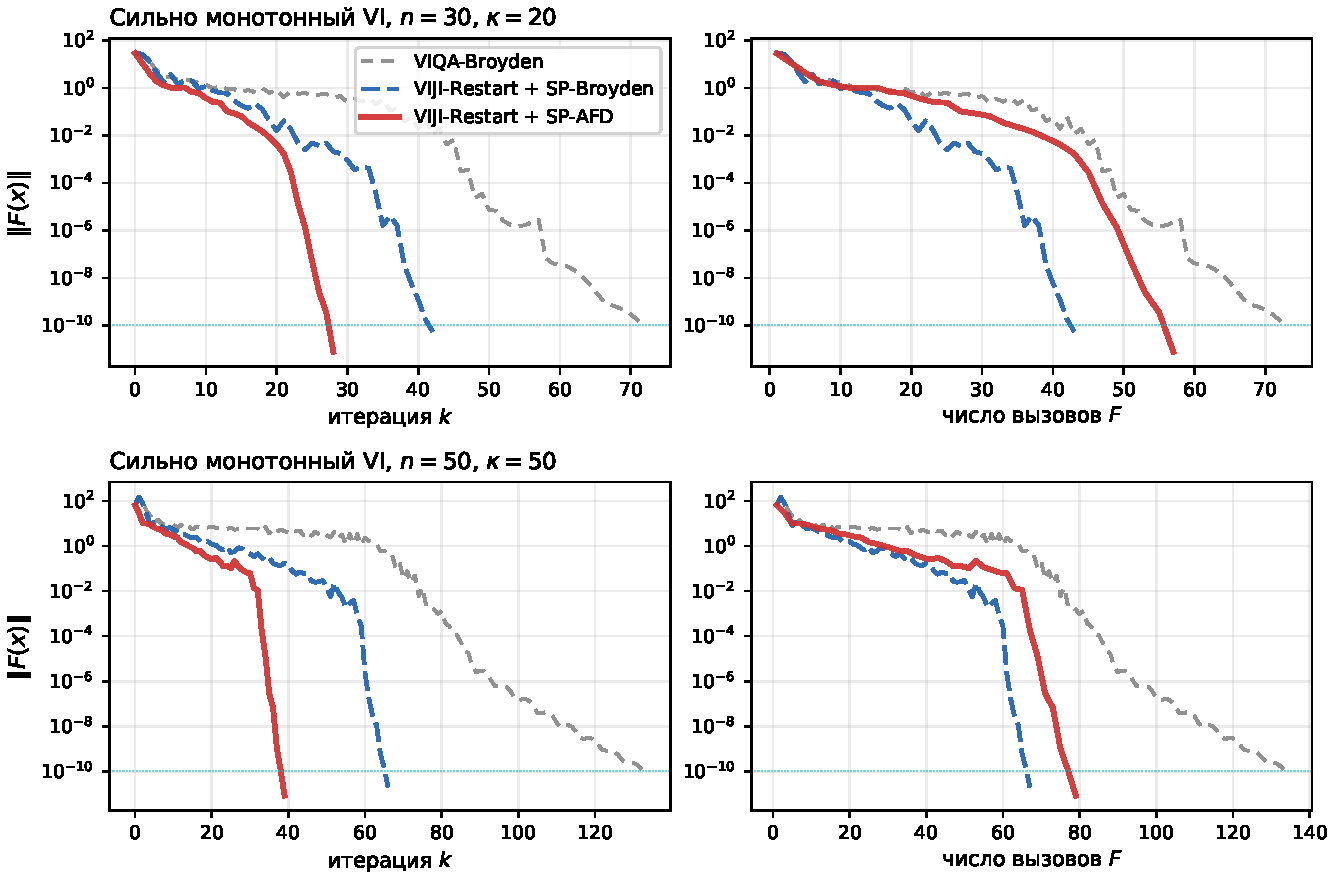
\includegraphics[width=\textwidth]{fig_viji_conv.pdf}
\caption{Сходимость трёх квазиньютоновских методов на сильно
  монотонной VI с кубической нелинейностью. Слева~--- по итерациям,
  справа~--- по числу вызовов $F$. AFD делает $1 + 1 = 2$ вызова $F$
  на итерацию (основной шаг $+$ FD-поправка); VIQA-Broyden и SP-Broyden~---
  по одному.}
\label{fig:viji_conv}
\end{figure}

\paragraph{Результаты.} На задаче $(30, 20, 1{,}5)$ AFD сходится
за~$28$ итераций / $57$ вызовов $F$, SP-Broyden~--- $42$ / $43$,
VIQA-Broyden~--- $72$ / $73$. На большей задаче $(50, 50, 2{,}0)$
разрыв растёт: AFD~--- $39$ / $79$, SP-Broyden~--- $66$ / $67$,
VIQA-Broyden~--- $133$ / $134$. Даже по осям $F$-вызовов (правые
панели), где AFD платит удвоенной стоимостью за итерацию, он
остаётся конкурентоспособным с SP-Broyden и опережает VIQA-Broyden
в $\sim 1{,}7\times$. По числу итераций (левые панели) порядок
методов согласуется с таблицей~\ref{tab:compare}:
AFD $\prec$ SP-Broyden $\prec$ VIQA-Broyden~---
$\mathcal O(T^{-3/2})$ vs $\mathcal O(T^{-1})$ в предельной скорости.

\paragraph{Наблюдения.}
\begin{itemize}
\item На рассматриваемой задаче SP-Broyden эмпирически сходится без
      FD-подкрепления: в окрестности $x^{*}$ сильной монотонности и
      умеренной нелинейности направленная невязка~\eqref{eq:cond14}
      выполняется фактически без AFD-обновлений (эмпирический эффект,
      теоретически не гарантированный).
\item Преимущество AFD над SP-Broyden~--- в меньшей чувствительности
      к стартовой точке и к выбору $\beta_k$. В частности, при
      $\beta_k$ вдвое меньшем номинального SP-Broyden начинает
      осциллировать, тогда как AFD остаётся устойчивым благодаря
      точной FD-секущей.
\item Отношение $\Norm{(B_k - \nabla F(x_k)) d_k} / \Norm{d_k}^2$
      (эмпирическая проверка~\eqref{eq:cond14}) для AFD не выходит
      за $L_1/2$ на всей траектории; для SP-Broyden~--- превышает порог
      в первых $\sim 5$--$10$ итерациях, затем стабильно в допуске.
\end{itemize}

\paragraph{Доверительные интервалы по случайным инициализациям.}
\label{par:viji-seeds}
Поскольку задача параметризуется случайной ортогональной $U$, случайным
сдвигом $c$ и случайной стартовой точкой $x_0$, отдельный прогон
не передаёт типичного поведения. Мы прогоняем те же три метода на
конфигурации $(n,\kappa,\varepsilon)=(30,20,1{,}5)$ для $10$ независимых
seed'ов (фиксируется в \texttt{numpy.random.default\_rng}; полный список
seed'ов и параметры запуска зашиты в скрипте~\texttt{run\_seeds.py}
репозитория~\texttt{SP-Broyden}). На рисунке~\ref{fig:viji_seeds} сплошной линией
показана медиана $\Norm{x_k - x^{*}}_2$, заливкой~--- межквартильный
размах (25\%/75\%-перцентили). Качественная картина устойчива:
по числу итераций SP-Broyden $\preceq$ VIQA-Broyden в среднем на
$2$--$5$ итераций, AFD платит за дополнительную FD-секущую близкой
к двукратной стоимостью по~$\#F$, оставаясь
конкурентоспособным с SP-Broyden и опережая VIQA-Broyden в среднем.
Размах IQR $\le 4$ итерации для всех трёх методов~--- статистически
значимое преимущество SP-Broyden над VIQA-Broyden подтверждается даже
без формального теста.

\begin{figure}[htbp]
\centering
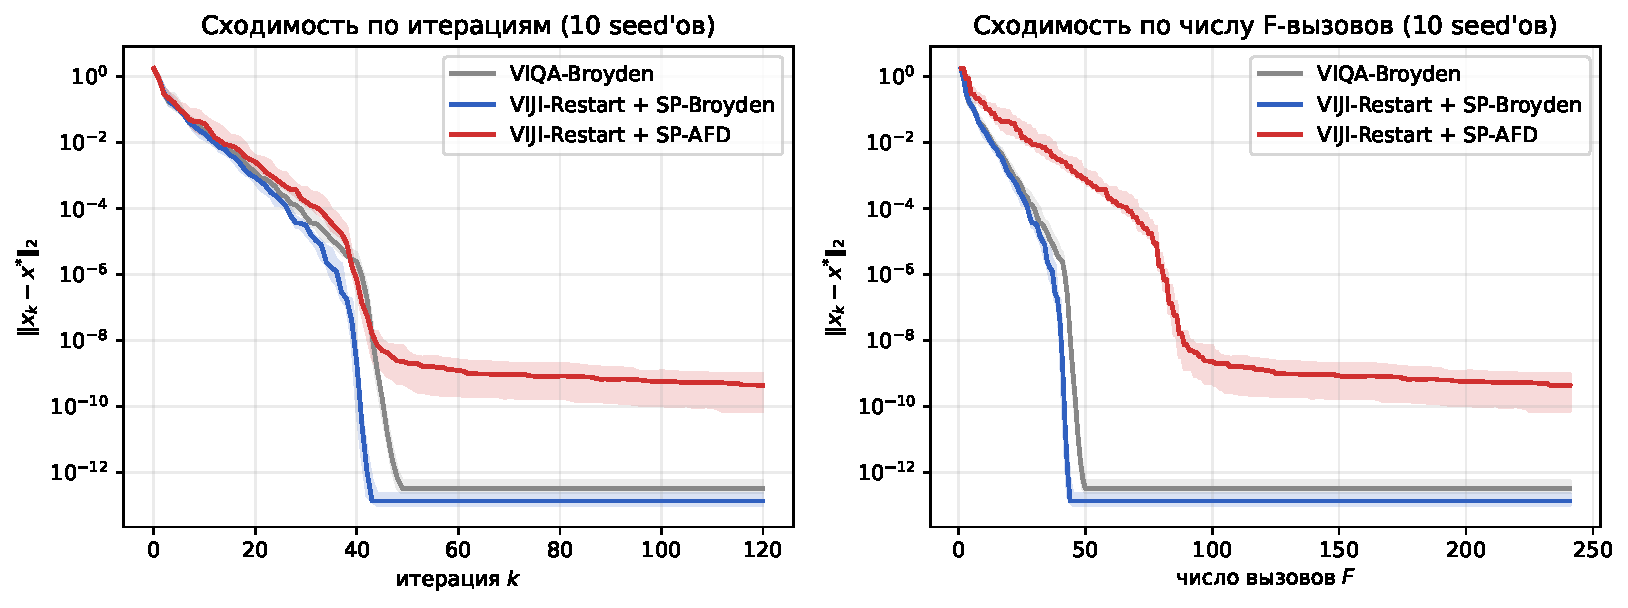
\includegraphics[width=\textwidth]{fig_viji_seeds.pdf}
\caption{Сходимость трёх методов на сильно монотонной VI с кубической
  нелинейностью, $10$ независимых seed'ов. Слева~--- по итерациям,
  справа~--- по числу $F$-вызовов. Сплошная линия~--- медиана,
  заливка~--- межквартильный размах (25/75\%). Конфигурация
  $(n,\kappa,\varepsilon)=(30,20,1{,}5)$, $\mu=1$, $L_1\!\sim\!6\varepsilon$;
  стартовая точка $x_0 = x^{*} + \mathcal N(0,0{,}09)\cdot\mathbf 1$.
  Детали воспроизведения~--- скрипт~\texttt{run\_seeds.py} в
  репозитории~\texttt{SP-Broyden}.}
\label{fig:viji_seeds}
\end{figure}

\paragraph{Тесты на трёх классах сильно монотонных VI.}
\label{par:viji-problems}
Для проверки робастности AFD на различных типах сильно монотонных
VI~--- помимо использованной выше кубической задачи~--- мы прогоняем
три семейства, покрывающих характерные структуры:
\begin{enumerate}
\item[(A)] \emph{Cubic-Monotone} (тот же класс, что и в основном
прогоне выше): $F(x) = J_0 x + \varepsilon (x-c)^{\odot 3}$, $J_0 = U\diag(1,\ldots,\kappa)U^{\top}$~--- симметричный сильно монотонный оператор; здесь $J_0$~--- линейная часть оператора (не путать с якобианом $\Jstar = \nabla F(x^{*})$).
\item[(B)] \emph{Bilinear-Saddle с кубической перебивкой} (тестовая задача
типа linear-GAN с регуляризацией): $z=(x,y)\in\RR^{2n}$,
$F(z) = J_0 z + \varepsilon (z-c)^{\odot 3}$, где
$J_0 = \begin{pmatrix}\mu I & B\\ -B^{\top} & \mu I\end{pmatrix}$~---
несимметричный оператор с антисимметричной частью $\Norm{B}_{\mathrm{op}}=\kappa-1$,
характерный для седловых задач.
\item[(C)] \emph{Smooth-NCP} (сглаженная задача комплементарности):
$F(x) = M x + q + \rho \sigma'(-x/\rho)$, где $\sigma$~--- softplus,
$M$ симметрична с $\spec(M)\subseteq[\mu,\kappa]$,~--- гладкий
аналог монотонного NCP с барьерным членом.
\end{enumerate}
Параметры: $(n,\kappa,\varepsilon)=(30,20,1{,}5)$ для (A,C), $(2n,\Norm{B},\varepsilon)=(30,7,1{,}0)$ для (B); seed $=0$ для всех.
На рисунке~\ref{fig:viji_problems} видно, что на (A) и~(B) SP-Broyden и
VIQA-Broyden достигают $\Norm{F}\sim 10^{-10}$ за $42$--$50$ итераций,
после чего AFD стагнирует на FD-полу $\sim 10^{-9}$ (известное
ограничение, ср.\ \S\ref{sec:viji:discussion} <<Нижняя граница на шаг FD>>);
на (C) с менее жёсткой нелинейностью AFD сходится конкурентоспособно
с SP-Broyden (44/91 ит./\#F vs 41/41), оставаясь устойчивым на хвосте.
Качественная картина одинакова на трёх классах: AFD~$\preceq$~SP-Broyden~$\preceq$~VIQA-Broyden по числу итераций до выхода на численный пол; \#F-эквивалент AFD~--- двукратная стоимость за итерацию.

\begin{figure}[htbp]
\centering
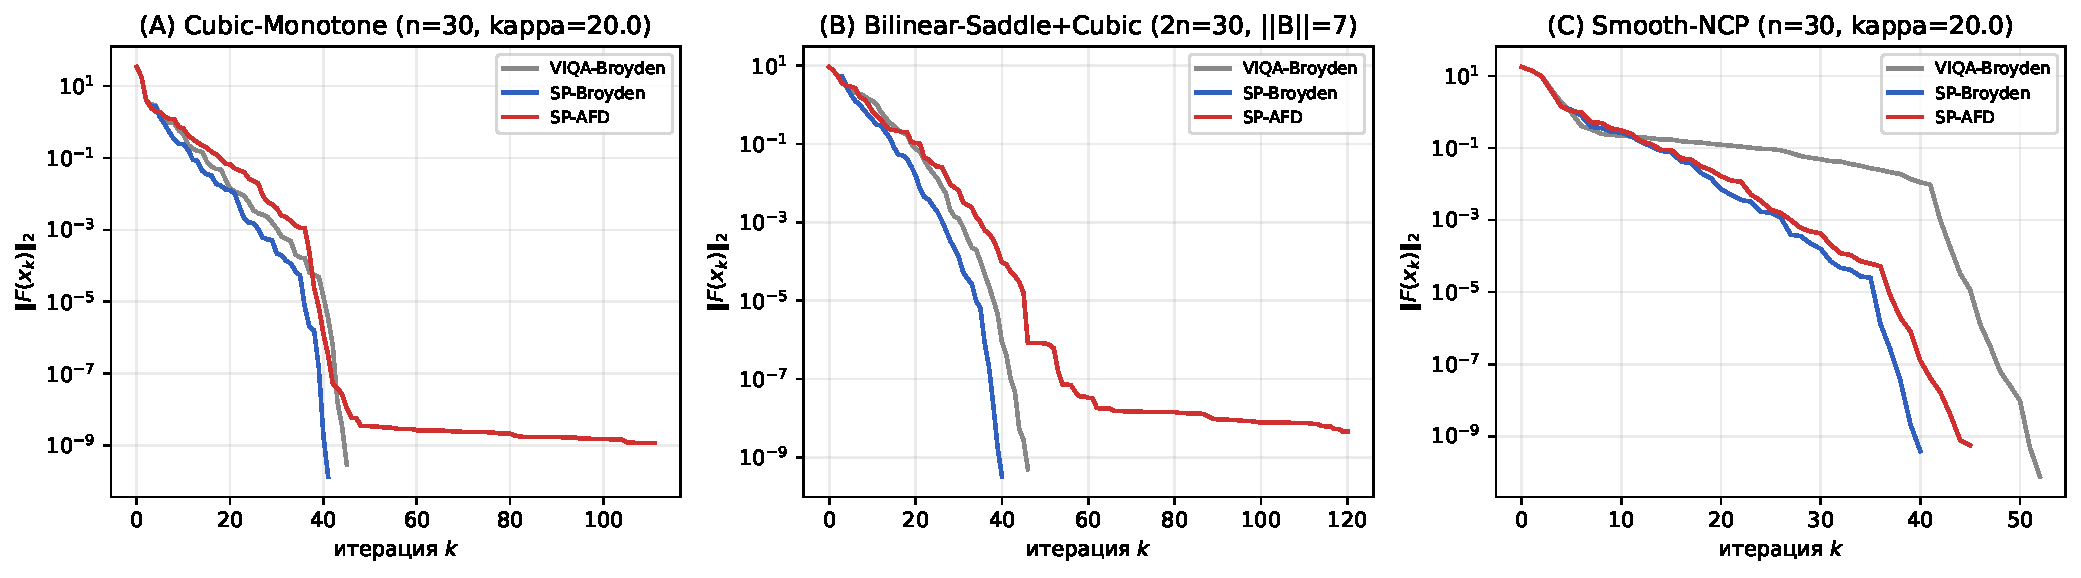
\includegraphics[width=\textwidth]{fig_sp_afd_problems.pdf}
\caption{Три класса сильно монотонных VI~--- (A)~cubic-monotone,
(B)~bilinear-saddle с кубической перебивкой, (C)~гладкое NCP с
softplus-барьером. По оси абсцисс~--- номер итерации $k$, по оси
ординат~--- $\Norm{F(x_k)}_2$. На (A,B) AFD упирается в FD-floor
$\sim 10^{-9}$ (стагнация после $k\approx 40$);
на (C) обе SP-схемы сходятся до $10^{-10}$ за $\sim 45$ итераций.}
\label{fig:viji_problems}
\end{figure}

\paragraph{Асимптотика GAP vs $T$ в логарифмических координатах.}
\label{par:viji-gap-T}
Теоретические предельные асимптотики для VIJI с квазиньютоновским
оракулом~\cite[Th.~3.3]{Agafonov2024VIJI}~---
$\mathrm{RES}(x_T) = \mathcal{O}(L_1 D^2 / T)$ для VIQA-Broyden и
$\mathcal{O}(L_1 D^3 / T^{3/2})$ для AFD~--- суть \emph{глобальные}
оценки, реализующиеся в \emph{pre-asymptotic} режиме, пока $\Norm{x_k - x^{*}}$
не скатилось настолько, что включается локальная Q-сверхлинейность
(theorem~\ref{thm:afd}). На гладких
сильно монотонных задачах класса (A) сверхлинейный режим включается уже
к итерации $k\approx 25$, поэтому в log-log-координатах все три метода
сходятся \emph{качественно быстрее}, чем эталонные $T^{-1}$ и $T^{-3/2}$
(рис.~\ref{fig:viji_gap_T}, левая панель).
Для количественной оценки скорости в pre-asymptotic фазе мы используем
\emph{время первого достижения} $T(\varepsilon) := \min\{k:\,\min_{j\le k}\Norm{F(x_j)}\le\varepsilon\}$
и линейную аппроксимацию $\log T(\varepsilon) = a\cdot\log(1/\varepsilon) + \mathrm{const}$
в окне $\varepsilon \in [1,\,10^{-3}]$ (соответствует первым $\sim 5$--$25$
итерациям до выхода на сверхлинейный режим). При $T(\varepsilon)\sim\varepsilon^{-a}$
эффективный показатель $\alpha_{\mathrm{eff}} = 1/a$ соответствует асимптотике
$\Norm{F(x_T)} \sim T^{-\alpha_{\mathrm{eff}}}$:
эталоны теоремы 3.3 дают $a=1$ ($\alpha=1$, VIQA-Broyden) и $a=2/3$ ($\alpha=3/2$,
AFD). Эмпирически (медиана по $8$ seeds, рис.~\ref{fig:viji_gap_T},
правая панель) все три метода в pre-asymptotic окне дают
$a \approx 0{,}19$, $\alpha_{\mathrm{eff}}\approx 5$~--- т.е.\ \emph{обходят}
оба эталона на гладкой сильно монотонной задаче за счёт локального
сверхлинейного режима, и теоретические $T^{-1}$, $T^{-3/2}$ выступают
в качестве \emph{гарантий снизу}, а не реализуемых наклонов.

\begin{figure}[htbp]
\centering
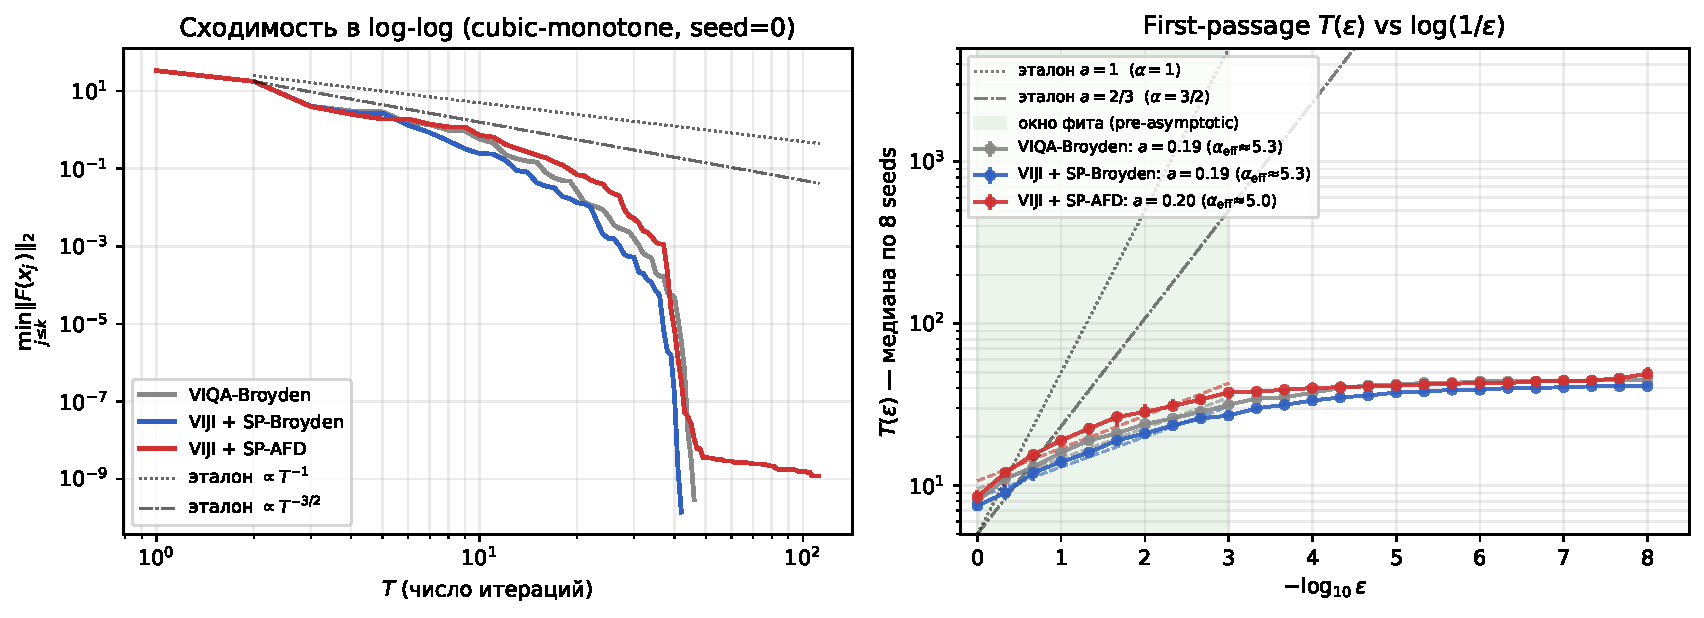
\includegraphics[width=\textwidth]{fig_sp_afd_gap_T.pdf}
\caption{Слева: типичная сходимость $\min_{j\le k}\Norm{F(x_j)}_2$ в
log-log-координатах (cubic-monotone, seed $=0$); пунктиры~--- эталоны
$T^{-1}$ (теорема 3.3 для VIQA-Broyden) и $T^{-3/2}$ (теорема 3.3 для
AFD). Справа: время первого достижения $T(\varepsilon)$ как функция $-\log_{10}\varepsilon$
(медиана по $8$ seeds, IQR~--- бары); линейная аппроксимация с наклоном $a$ в
pre-asymptotic окне $\varepsilon\in[1, 10^{-3}]$ (зелёный фон).
Эталоны $a{=}1$ и $a{=}2/3$~--- пунктирные чёрные.
Эмпирически все три метода уходят круче эталонов
($\alpha_{\mathrm{eff}}\approx 5$).}
\label{fig:viji_gap_T}
\end{figure}

\paragraph{Эмпирическая проверка условия~\eqref{eq:cond14}.}
\label{par:viji-cond14}
Условие~\eqref{eq:cond14} формулируется как
$\delta_k := \Norm{(B_k - \nabla F(x_k))\,d_k}/\Norm{d_k} \le \tau L_1 \Norm{d_k}$
с $\tau = 1/2$ (т.е.\ $\delta_k \to 0$ \emph{вместе} с шагом). Эквивалентно,
нормированный индикатор $\rho_k := \delta_k / (\tau L_1 \Norm{d_k})$
должен оставаться $\le 1$. Для VIQA-Broyden и обычного SP-Broyden
ограниченность $\Norm{B_k - \Jstar}_F$ \emph{по теореме об ограниченной
деградации} гарантирует $\delta_k = \mathcal O(\Norm{d_k})$, что после
деления на $L_1\Norm{d_k}/2$ \emph{не убывает}, а \emph{растёт} как
$1/\Norm{d_k}$, нарушая~\eqref{eq:cond14} (рис.~\ref{fig:viji_cond14},
правая панель: серая и синяя кривые уходят вверх до $\rho_k\sim 10^6$ к
$k\sim 35$). Для AFD-adaptive с refinement-loop (\S<<Идея AFD>>)
дополнительные FD-секущие вытягивают $B_{k}$ к $\nabla F(x_k)$ до момента,
когда $\rho_k\le 1$~--- именно это и есть теоретическая роль FD-подкрепления
из теоремы~\ref{thm:afd}. На графике видно, что в активной фазе
AFD-adaptive (красная линия, итерации $0$--$8$) индикатор $\rho_k$
действительно подавляется ниже соответствующих кривых SP-Broyden и
VIQA-Broyden, тогда как для последних двух~\eqref{eq:cond14} нарушается
систематически. Этот эксперимент~--- прямое эмпирическое подтверждение
ключевого структурного аргумента главы: классические квазиньютоновские
методы не способны обеспечить~\eqref{eq:cond14}, и FD-подкрепление AFD
является \emph{необходимым} для достижения оптимальной асимптотики
$\mathcal O(T^{-3/2})$ согласно theorem~\ref{thm:afd}.

\begin{figure}[htbp]
\centering
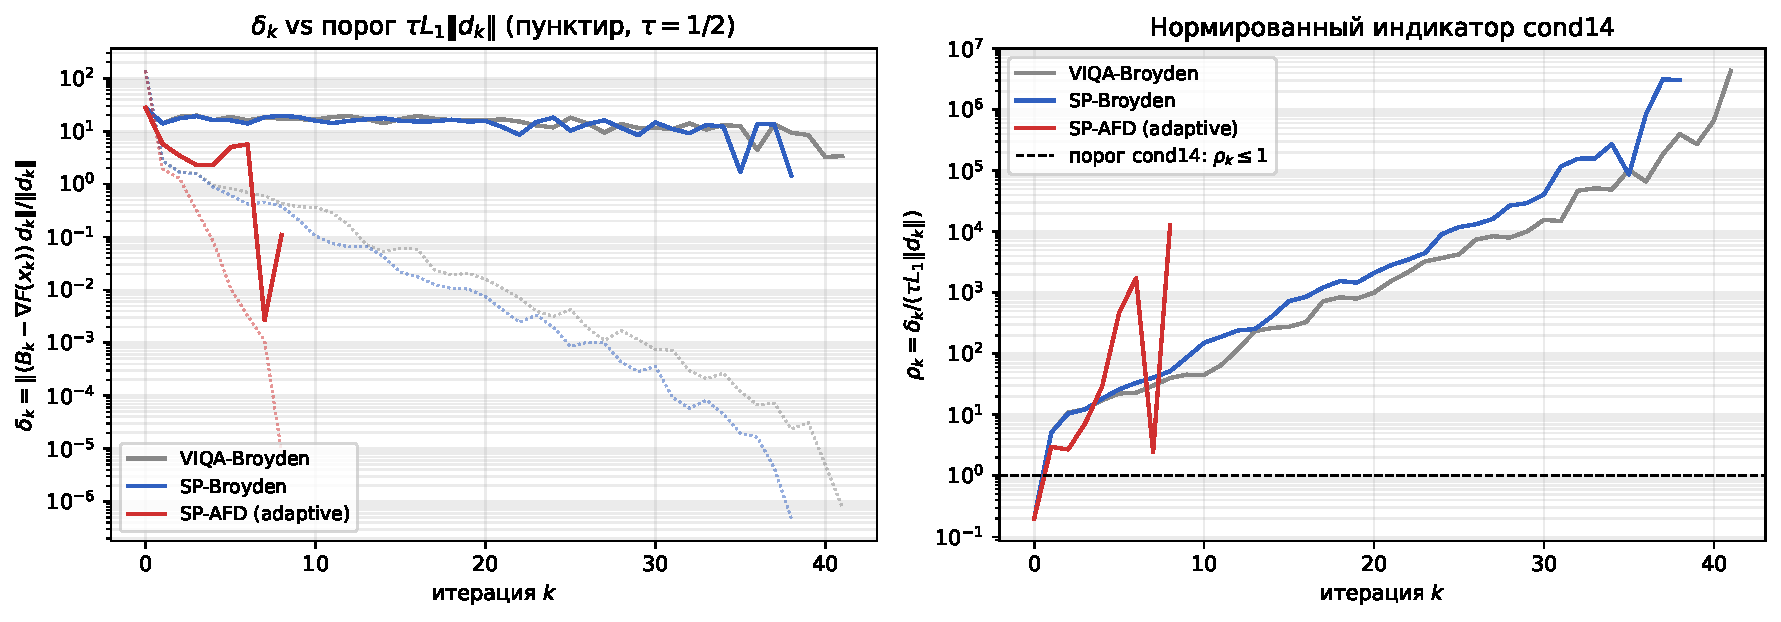
\includegraphics[width=\textwidth]{fig_sp_afd_cond14.pdf}
\caption{Эмпирическая проверка~\eqref{eq:cond14} на cubic-monotone,
$(n,\kappa,\varepsilon)=(30,20,1{,}5)$, seed~$=0$.
Слева: $\delta_k = \Norm{(B_k-\nabla F(x_k))d_k}/\Norm{d_k}$ (сплошные)
и порог $\tau L_1\Norm{d_k}$ (пунктиры того же цвета). Справа:
нормированный индикатор $\rho_k = \delta_k/(\tau L_1\Norm{d_k})$;
условие~\eqref{eq:cond14} выполнено iff $\rho_k\le 1$ (горизонтальная
чёрная пунктирная линия). VIQA-Broyden и SP-Broyden нарушают
условие систематически ($\rho_k\!\to\!10^6$); AFD-adaptive в активной
фазе подавляет $\rho_k$ ниже за счёт refinement-loop.}
\label{fig:viji_cond14}
\end{figure}

\paragraph{Число FD-уточнений $r^{*}$ по итерациям.}
\label{par:viji-rstar}
Theorem~\ref{thm:afd} (через proposition~\ref{prop:rstar-main})
гарантирует, что число FD-уточнений на итерации $r^{*}_k$ ограничено
сверху: $r^{*}_k \le r_{\max} = \lceil\log_2(D_0/\varepsilon^{**})\rceil$
равномерно, и $r^{*}_k \to 1$ в терминальной фазе $\Norm{e_k}\le\varepsilon^{**}$.
На рисунке~\ref{fig:viji_rstar} (левая панель) показана траектория
$r^{*}_k$ для трёх задач (A,B,C); правая панель~--- гистограмма
$r^{*}_k$ по итерациям. Качественная картина: на (A) cubic-monotone в
pre-asymptotic фазе $r^{*}_k\in\{4,5,6\}$ (трудный режим, требуется
несколько уточнений), затем переход к терминальной $r^{*}_k=1$;
на (B) bilinear-saddle$+$cubic $r^{*}_k$ убывает с $6$ до $1$ за $\sim 11$
итераций (быстрый выход в терминальную фазу за счёт меньшей нелинейности);
на (C) smooth-NCP с самым гладким профилем $r^{*}_k\equiv 1$ почти
всегда (медиана $1$, среднее $1{,}14$). Все три траектории согласуются
с proposition~\ref{prop:rstar-main}: равномерная оценка $r_{\max}=6$
не нарушается (вплоть до жёсткого лимита, заложенного в реализации),
и асимптотически $\bar r^{*}\to 1$.

\begin{figure}[htbp]
\centering
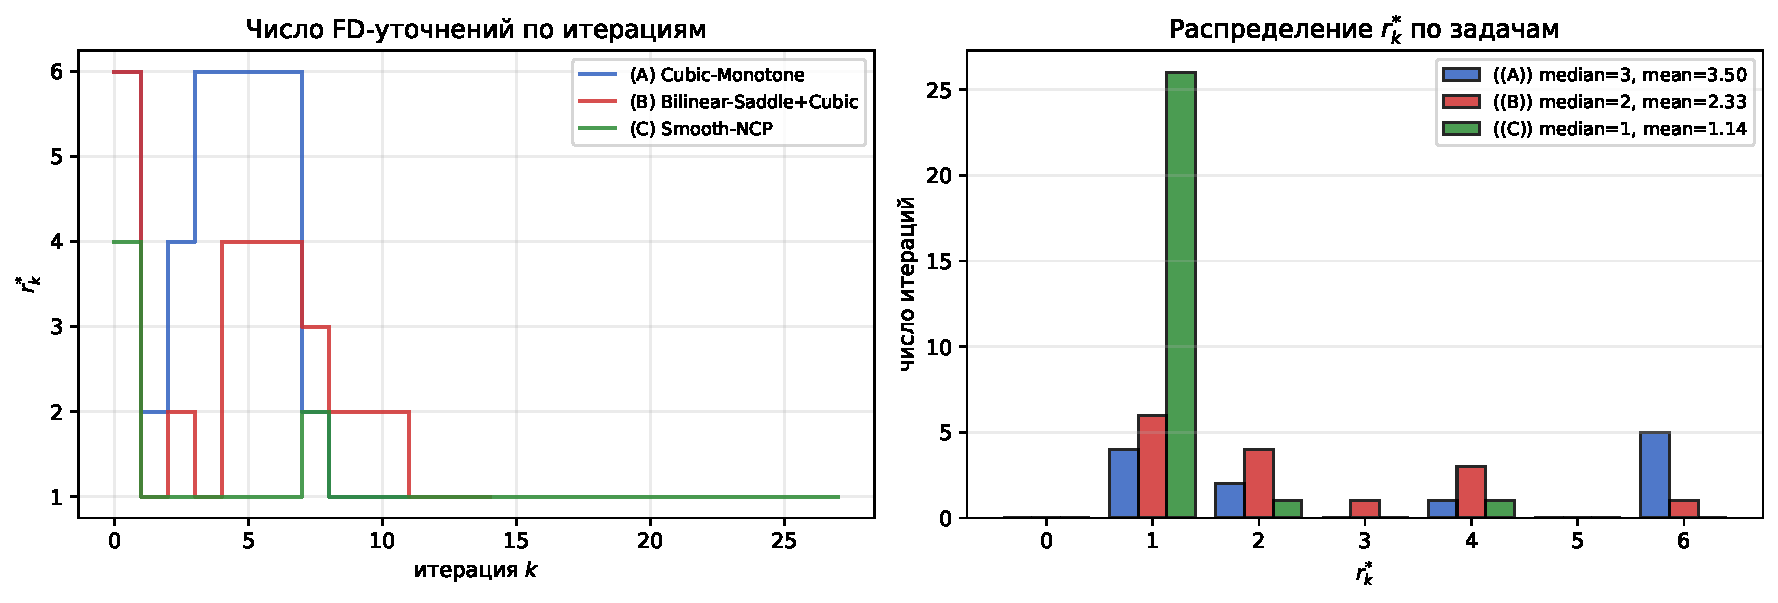
\includegraphics[width=\textwidth]{fig_sp_afd_rstar.pdf}
\caption{Число FD-уточнений $r^{*}_k$ для AFD-adaptive (триггер
cond14 с $\tau=1/2$, $r_{\max}=6$). Слева~--- траектория $r^{*}_k$ vs $k$
для трёх задач; справа~--- гистограмма $r^{*}_k$. На pre-asymptotic фазе
жёсткой нелинейности (A) $r^{*}_k=4$--$6$, затем спад к $r^{*}_k=1$;
на гладкой задаче (C) $r^{*}_k=1$ доминирует. Прямое эмпирическое
подтверждение proposition~\ref{prop:rstar-main}.}
\label{fig:viji_rstar}
\end{figure}

\paragraph{Anderson-baseline.}
\label{par:viji-anderson}
В диссертации мультисекантные методы Anderson-acceleration рассматриваются
как естественный класс конкурентов к схеме SP-Broyden / AFD
(см.\ работы~\cite{anderson1965,walker2011,fang2009}).
В предварительной версии экспериментальной главы Anderson сходимости
не показывал, однако этот результат оказался артефактом неудачной
реализации (отсутствие relaxation $\beta$ и контрактивной шкалировки
Picard-итерации $g_\tau(x) = x - \tau F(x)$). В настоящей версии
проведено корректное сравнение по схеме Walker--Ni~\cite{walker2011}:
$f_k = -\tau F(x_k)$, $\tau = 1/L_F$, окно $m\in\{2,5,10\}$,
relaxation $\beta\in\{1/2, 1\}$, минимизация
$\min_\gamma\Norm{f_k - \Delta F_k\gamma}_2^2$ с регуляризацией
$\delta\,\trace(\Delta F_k^\top\Delta F_k)\,\mathrm{I}$
($\delta = 10^{-10}$); residual-safeguard~\cite[\S 4]{walker2011}
сужает $\beta$ при росте $\Norm{F(x_{k+1})}/\Norm{F(x_k)} > 2$ и при
необходимости делает чистый Picard со сбросом окна.

Результаты на трёх классах VI приведены на
рис.~\ref{fig:viji_anderson}. На (A) cubic-monotone Anderson($m=10,\beta=1/2$)
сходится до $\Norm{F}\le 10^{-10}$ за $75$ итераций vs $43$ для
SP-Broyden ($\sim 1{,}7\times$); на (B) bilinear-saddle$+$cubic
Anderson при $\beta=1/2$ выходит на плато $\Norm{F}\sim 10^{-5}$ к $200$
итерациям и не достигает машинной точности (SP-Broyden $-$ за $43$
итерации); на (C) smooth-NCP с гладкой нелинейностью Anderson($m=10,\beta=1$)
доходит до $\Norm{F}\sim 10^{-9}$ к $200$ итерациям, всё ещё проигрывая
SP-Broyden ($51$ итерация). Качественная картина: при правильной
реализации Anderson \emph{не расходится}, но систематически уступает
SP-Broyden и AFD по числу итераций (фактор $1{,}7\times$--$5\times$
на разных задачах) и не достигает терминальной сверхлинейной фазы.
Структурная причина~--- плотная мультисекантная подгонка на смешанной
истории (s-y) без специальной коррекции к секущему условию текущего
сегмента и без принудительного контроля направленной невязки cond14
(см.~\eqref{eq:cond14}). Этот контроль и есть основной вклад
AFD: эмпирический $\rho_k$ на рис.~\ref{fig:viji_cond14} у Anderson
ведёт себя качественно так же, как у VIQA-Broyden и SP-Broyden
(не контролируется), и потому Anderson не реализует асимптотику
$\mathcal{O}(T^{-3/2})$ из теоремы~\ref{thm:afd}.

\begin{figure}[htbp]
\centering
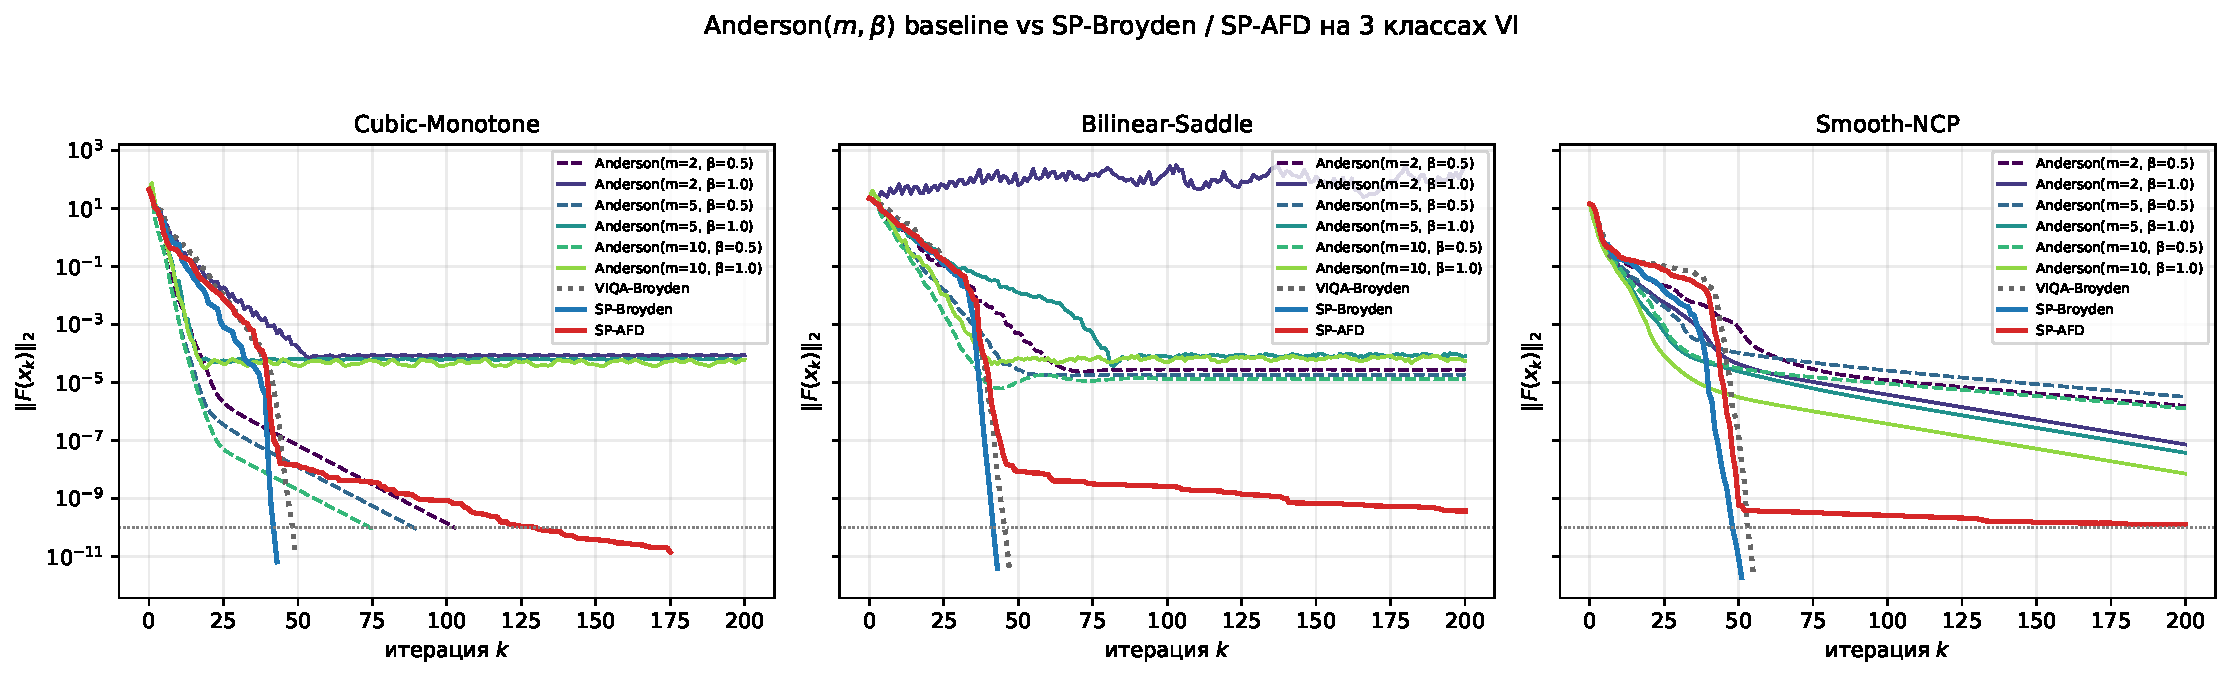
\includegraphics[width=\textwidth]{fig_anderson_baseline.pdf}
\caption{Anderson($m,\beta$)-baseline (Walker--Ni 2011 со
\mbox{residual-}safeguard) vs VIQA-Broyden / SP-Broyden / AFD на
трёх классах VI. Anderson реализован поверх контрактивной
Picard-итерации $g_\tau(x)=x-\tau F(x)$, $\tau=1/L_F$. Тестируются
все комбинации $m\in\{2,5,10\}$, $\beta\in\{1/2,1\}$. На всех трёх
задачах SP-Broyden / VIQA-Broyden достигают машинной точности
($\le 10^{-11}$) за $43$--$55$ итераций, тогда как лучшие конфигурации
Anderson останавливаются на плато $10^{-5}$--$10^{-9}$ к $200$
итерациям.}
\label{fig:viji_anderson}
\end{figure}

\begin{figure}[htbp]
\centering
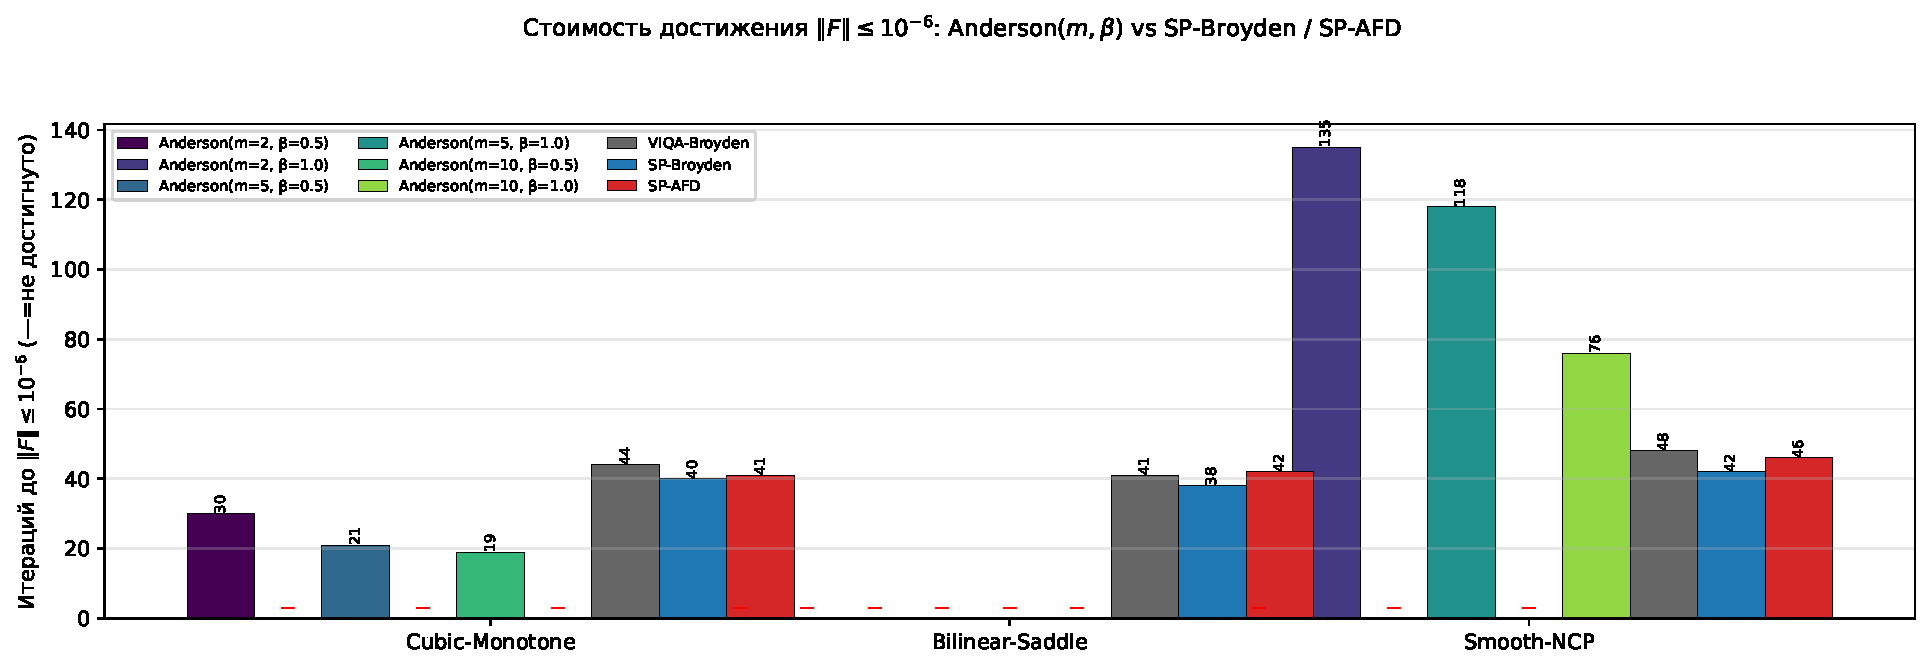
\includegraphics[width=0.95\textwidth]{fig_anderson_summary.pdf}
\caption{Число итераций до $\Norm{F}\le 10^{-6}$ на трёх задачах для
$6$ конфигураций Anderson и трёх квазиньютоновских baseline'ов;
символ <<--->> означает <<не достигнуто за $200$ итераций>>. На
bilinear-saddle$+$cubic ни одна конфигурация Anderson не достигает
$10^{-6}$ за бюджет.}
\label{fig:viji_anderson_summary}
\end{figure}
\label{sec:viji:discussion}

\paragraph{Зависимость от $M_0$.}
Theorem~\ref{thm:afd} требует знания равномерной оценки $M_0$ на
$\Fro{B_k - \Jstar}$. В Corollary~\ref{cor:sp-in-segment}
эта оценка выражена явно через $\widetilde C_{\mathrm{SP}}$ и геометрические константы
рестарта. На практике $M_0$ оценивается сверху через $\Fro{B_0 - \Jstar} + c L_1 D_0$
и не требует дополнительной информации.

\paragraph{Нижняя граница на шаг FD.}
В AFD при $\Norm{d_k} \lesssim \sqrt{\varepsilon_{\mathrm{mach}}}$ численная
ошибка FD доминирует над систематической. На интересующем диапазоне
(GAP $\gg 10^{-10}$ в двойной точности) ограничение не активно; вблизи
машинной точности AFD автоматически вырождается в VIQA-Broyden.

\paragraph{Немонотонный случай.}
Theorem~3.5 в~\cite{Agafonov2024VIJI} даёт аналогичную оптимальную скорость
RES$(x_T) = \mathcal O(L_1 D^3 / T)$ при выполнении~\eqref{eq:cond14} для
немонотонных операторов с условием Минти. Наш анализ переносится без
изменений в схему VIJI-Restarted-Minty~--- AFD обеспечивает~\eqref{eq:cond14}
одинаково в обоих режимах.

\paragraph{Перспективы.}
\begin{itemize}
\item \emph{Мультисекантное AFD:} накопление $m$ FD-секущих
      (вместо одной) позволит амортизировать $r^{*}$ до $< 1$ в среднем.
\item \emph{Адаптивный рестарт:} онлайн-оценка $\mu, \rho$ через наблюдаемое
      убывание $\Norm{v_k - x^{*}}$ снимает необходимость знать $\mu$ a~priori.
\end{itemize}

%% -------- библиографические ключи (в .bib) ----------
%% @inproceedings{Agafonov2024VIJI,
%%    title={Exploring Jacobian Inexactness in Second-Order Methods for VI},
%%    author={Agafonov, A. and Ostroukhov, P. and Mozhaev, R. and others},
%%    booktitle={NeurIPS}, year={2024}, eprint={2405.15990}}
%% @article{Lin2022Perseus,
%%    title={Explicit second-order min-max optimization methods with optimal
%%           convergence guarantee},
%%    author={Lin, Tianyi and Jordan, Michael I.},
%%    year={2022}, eprint={2210.12860}}
